\documentclass[letterpaper,12pt,oneside,final]{book}
%%
%%  Gabarit bilingue de mémoire de maîtrise ou thèse de doctorat.
%%  Bilingual template for dissertations and theses @ Polytechnique Montreal.

%%  Normalement, il n'est pas nécessaire de modifier ce document
%%  sauf pour établir le langage (français ou anglais) et pour changer les noms des fichiers à inclure.
%%  Usually, this document needs to be modified only to set up the language (French or English) and to change the names of the files to include.
%%
%%  Version: 2023-01-20
%%
%% Accepte les caractères accentués dans le document (UTF-8).
%% Supports accented characters in the document (UTF-8).


%\makeatletter
%\def\bstctlcite{\@ifnextchar[{\@bstctlcite}{\@bstctlcite[@auxout]}}
%\def\@bstctlcite[#1]#2{\@bsphack
% \@for\@citeb:=#2\do{%
%   \edef\@citeb{\expandafter\@firstofone\@citeb}%
%   \if@filesw\immediate\write\csname #1\endcsname{\string\citation{\@citeb}}\fi}%
% \@esphack}
%\makeatother

%% LA COMMANDE SUIVANTE ÉTABLIT LE LANGAGE DE LA THÈSE : ÉCRIRE french POUR UNE THÈSE EN FRANÇAIS
%% THE NEXT COMMAND DETERMINES THE LANGUAGE OF THE THESIS: WRITE english FOR A THESIS IN ENGLISH
\newcommand\Langue{french}            
%%\makeatletter\newcommand{\set@color}{\message{DEBUG \the\inputlineno}}\makeatother
\usepackage{ifthen}
\usepackage[utf8]{inputenc}
%%
%% Support pour l'anglais et le français (français par défaut).
%% Support for English and French (French by default).

%\usepackage[cyr]{aeguill}
\usepackage{lmodern}      % Police de caractères plus complète et généralement indistinguable visuellement de la police standard de LaTeX (Computer Modern). / A more complete and generally visually indistinguishable font from the standard LaTeX font (Computer Modern).
\usepackage[T1]{fontenc}  % Bon encodage des caractères pour qu'Acrobat Reader reconnaisse les accents et les ligatures telles que ffi. / Good character encoding so that Acrobat Reader recognizes accents and ligatures such as ffi.

\ifthenelse{\equal{\Langue}{english}}{
	\usepackage[french,english]{babel}
}{
	\usepackage[english,french]{babel} 
}
\usepackage[style=apa, backend=biber]{biblatex}
\addbibresource{Maitrise_recherche.bib}
\DeclareLanguageMapping{french}{french-apa}
\DefineBibliographyExtras{french}{\restorecommand\mkbibnamefamily}
\DeclareDelimFormat[bib]{finalnamedelim}{
    \ifthenelse{\value{listcount}>\maxprtauth}
    {}
    {\ifthenelse{\ifcurrentname{groupauthor}\AND%
            \value{liststop}=2}
        {\addspace\bibstring{et}\space}
        {\finalandcomma\addspace\bibstring{et}\space}}}
%%
%% Charge le module d'affichage graphique. / Loads the graphics package.
\usepackage{graphicx}
\usepackage{epstopdf}  % Permet d'utiliser des .eps avec pdfLaTeX. / Allows using .eps with pdfLaTeX.
%%
%% Recherche des images dans les répertoires. / Search for images in folders.
\graphicspath{{./images/}{./dia/}{./gnuplot/}}
%%
%% Un float peut apparaître seulement après sa définition, jamais avant. / A float can appear only after its definition, never before.
\usepackage{flafter,placeins}
%%
%% Autres modules. / Other packages.
\usepackage{amsmath,color,soulutf8,longtable,colortbl,setspace,xspace,url,pdflscape,amsthm,multirow,rotating,neuralnetwork,tikz,makecell,bbding,xcolor,array,pgfplots,pgfplotstable}
\pgfplotsset{compat=1.9}
\usetikzlibrary{fadings}
\usetikzlibrary{decorations.pathreplacing}
\usepackage{sidecap}
\newtheorem{definition}{Définition}
\newcommand{\STAB}[1]{\begin{tabular}{@{}c@{}}#1\end{tabular}}
%%
%% Support des acronymes. / Support for acronyms.
\usepackage[nolist]{acronym}
\onehalfspacing                % Interligne 1.5. / Line spacing = 1.5.
%%
%% Définition d'un style de page avec seulement le numéro de page à
%% droite. On s'assure aussi que le style de page par défaut soit
%% d'afficher le numéro de page en haut à droite. / Definition of a page 
%% style with only the page number on the right. We also make sure that the 
%% default page style is to display the page number at the top right.

\usepackage{fancyhdr}
\fancypagestyle{pagenumber}{\fancyhf{}\fancyhead[R]{\thepage}}
\renewcommand\headrulewidth{0pt}
\makeatletter
\let\ps@plain=\ps@pagenumber
\makeatother
%%
%% Module qui permet la création des bookmarks dans un fichier PDF. / Package that allows the creation of bookmarks in a PDF file.
%\usepackage[dvipdfm]{hyperref}
\usepackage{hyperref}
\usepackage{caption}  % Hyperlien vers la figure plutôt que son titre. / Hyperlink to the figure rather than its title.
\makeatletter
\providecommand*{\toclevel@compteur}{0}
\makeatother

%% Modules ajoutés (2022) / packages added (2022)
\usepackage{subcaption} % figures & sous figures / figures & subfigures
\usepackage{siunitx} % unites SI / SI units
\usepackage{amssymb} % autres symboles mathematiques / other mathematical symbols
\usepackage[bottom]{footmisc} % pour avoir les notes de bas de page en dessous des figures... / to have the footnotes below the figures
%\usepackage{listings} % Si on veut ajouter des lignes de codes dans le texte / If you want to add lines of code to the text


%%
%% Définitions spécifiques au format de rédaction de Poly.
%% Here we define the Poly formatting.
\RequirePackage[\Langue]{MemoireThese}
%%
%% Définitions spécifiques à l'étudiant.
%% Student-specific definitions.
%% -----------------------------------
%% ---> À MODIFIER PAR L'ETUDIANT / TO BE MODIFIED BY THE STUDENT <---
%% -----------------------------------
%%
%% Commandes qui affichent le titre du document, le nom de l'auteur, etc.
% Commands that display the document title, the author's name, etc.
\newcommand\monTitre{Inventaire de l'offre de stationnement \\ de la ville de Québec}
\newcommand\monPrenom{Paul}
\newcommand\monNom{Charbonneau}
\newcommand\monDepartement{Génie civil et des mines}  % Department
\newcommand\maDiscipline{Génie civil}
\newcommand\monDiplome{M}        % (M)aîtrise ou (D)octorat / (M)aster or Ph(D)
\newcommand\anneeDepot{2025}    % Year
\newcommand\moisDepot{Juin}       % Month
\newcommand\monSexe{M}           % "M" ou "F" = Gender
\newcommand\PageGarde{O}         % "O" ou "N" = Yes or No
\newcommand\AnnexesPresentes{N}  % "O" ou "N". Indique si le document comprend des annexes. / If the thesis includes annexes = O; if it does not N = No.
\newcommand\mesMotsClef{Liste,de,mot-clés,séparés,par,des,virgules}
%%
%%  DEFINITION DU / OF JURY
%%
%%  Pour la définition du jury, les macros suivantes sont definies: / For the definition of the jury, the following macros are defined:
%%  \PresidentJury, \DirecteurRecherche, \CoDirecteurRecherche, \MembreJury, \MembreExterneJury
%%
%%  Toutes les macros prennent 3 paramètres: Sexe (M/F), Nom, Prénom
%%  All the macros have 3 parameters: Gender (M/F), Last name, First name
\newcommand\monJury{\PresidentJury{M}{TBD}{TBD}\\
\DirecteurRecherche{F}{Morency}{Catherine}\\
\CoDirecteurRecherche{F}{TBD}{TBD}\\
\MembreJury{M}{TBD}{TBD}\\
\MembreExterneJury{M}{TBD}{TBD}}


\ifthenelse{\equal{\monDiplome}{M}}{
  \newcommand\monSujet{Mémoire de maîtrise}
  \newcommand\monDipl{Maîtrise ès sciences appliquées}
}{
  \newcommand\monSujet{Thèse de doctorat}
  \newcommand\monDipl{Philosophi\ae{} Doctor}
}
%%
%% Informations qui sont stockées dans un fichier PDF.
%% Information that is stored in a PDF file.
\hypersetup{
  pdftitle={\monTitre},
  pdfsubject={\monSujet},
  pdfauthor={\monPrenom{} \monNom},
  pdfkeywords={\mesMotsClef},
  bookmarksnumbered,
  pdfstartview={FitV},
  hidelinks,
  linktoc=all
}

%% Ajoute en 2022 (ajout des titres complets des tables et figure et alignement)
%% Added in 2022 (added full table and figure titles and alignment)
\usepackage[titles]{tocloft}
  \renewcommand{\cftchapleader}{\cftdotfill{\cftsecdotsep}} % dotted chapter leaders

\renewcommand\cfttabindent{0pt}
\renewcommand\cfttabnumwidth{7em}
\renewcommand\cfttabpresnum{\tablename\ }

\renewcommand\cftfigindent{0pt} 
\renewcommand\cftfignumwidth{7em}
\renewcommand\cftfigpresnum{\figurename\ }

\ifthenelse{\equal{\Langue}{english}}{
	\renewcommand\cftchapfont{CHAPTER }
    \renewcommand\cftchappagefont{}
}{
	\renewcommand\cftchapfont{CHAPITRE }
    \renewcommand\cftchappagefont{}
}
%

%%
%% Il y a un document par chapitre du mémoire ou thèse.
%% There is one document per chapter of the thesis or dissertation.

\begin{document}
%\bstctlcite{IEEEexample:BSTcontrol}

%%
%% Page de titre du mémoire ou de la thèse.
%% Title page of the dissertation or thesis.
\frontmatter
%% Compte optionellement la page de garde dans la pagination.
%% Optionally counts the cover page in the pagination.
\ifthenelse{\equal{\PageGarde}{O}}{\addtocounter{page}{1}}{}
\thispagestyle{empty}%
\begin{center}%
\vspace*{\stretch{0.1}}
\textbf{POLYTECHNIQUE MONTRÉAL}\\
affiliée à l'Université de Montréal\\
\vspace*{\stretch{1}}
\textbf{\monTitre}\\
\vspace*{\stretch{1}}
\textbf{\MakeUppercase{\monPrenom~\monNom}}\\
Département de~{\monDepartement}\\
\vspace*{\stretch{1}}
\ifthenelse{\equal{\monDiplome}{M}}{Mémoire présenté}{Thèse présentée} en vue de l'obtention du diplôme de~\emph{\monDipl}\\
\maDiscipline\\
\vskip 0.4in
\moisDepot~\anneeDepot
\end{center}%
\vspace*{\stretch{1}}
\copyright~\monPrenom~\monNom, \anneeDepot.
%%
%% Identification des membres du jury.
%% Jury members.
\newpage\thispagestyle{empty}%
\begin{center}%

\vspace*{\stretch{0.1}}
\textbf{POLYTECHNIQUE MONTRÉAL}\\
affiliée à l'Université de Montréal\\
\vspace*{\stretch{2}}
Ce\ifthenelse{\equal{\monDiplome}{M}}{~mémoire intitulé}{tte thèse intitulée} :\\
\vspace*{\stretch{1}}
\textbf{\monTitre}\\
\vspace*{\stretch{1}}
présenté\ifthenelse{\equal{\monDiplome}{M}}{}{e}
par~\textbf{\mbox{\monPrenom~\MakeUppercase{\monNom}}}\\
en vue de l'obtention du diplôme de~\emph{\mbox{\monDipl}}\\
a été dûment accepté\ifthenelse{\equal{\monDiplome}{M}}{}{e} par le jury d'examen constitué de :\end{center}
\vspace*{\stretch{2}}
\monJury
%%
\pagestyle{pagenumber}%
%% Dédicace
%%
%% La dédicace est un hommage que l'auteur souhaite
%% rendre à une ou plusieurs personnes de son choix.
%%
%% The dedication is a tribute to one or more persons of choice.
\ifthenelse{\equal{\Langue}{english}}{
	\chapter*{DEDICATION}\thispagestyle{headings}
	\addcontentsline{toc}{compteur}{DEDICATION}
}{
	\chapter*{DÉDICACE}\thispagestyle{headings}
	\addcontentsline{toc}{compteur}{DÉDICACE}
}

\begin{flushright}
  \itshape
  TBD\\
  TBD\ldots
\end{flushright}
          % Dédicace du document.
% Remerciements / Acknowledgements
%
% Grâce aux remerciements, l'auteur attire l'attention du 
% lecteur sur l'aide que certaines personnes lui ont apportée, 
% sur leurs conseils ou sur toute autre forme de contribution 
% lors de la réalisation de son mémoire ou thèse. Le cas 
% échéant, c'est dans cette section que le candidat doit 
% témoigner sa reconnaissance à son directeur de recherche, aux 
% organismes dispensateurs de subventions ou aux entreprises qui
% lui ont accordé des bourses ou des fonds de recherche.

% Through the acknowledgements, the author draws the
% reader's attention to the help that certain people 
% have given them, their advice or any other form of 
% contribution during the completion of the 
% dissertation or thesis. If applicable, it is in 
% this section the candidate should acknowledge the 
% assistance of their advisor, granting agencies or 
% companies that have provided research grants or
% funds.
\ifthenelse{\equal{\Langue}{english}}{
	\chapter*{ACKNOWLEDGEMENTS}\thispagestyle{headings}
	\addcontentsline{toc}{compteur}{ACKNOWLEDGEMENTS}
}{
	\chapter*{REMERCIEMENTS}\thispagestyle{headings}
	\addcontentsline{toc}{compteur}{REMERCIEMENTS}
}
%
Texte / Text.
     % Remerciements / Acknowledments
% Résumé du mémoire.
% Abstract in French.
%
\chapter*{RÉSUMÉ}\thispagestyle{headings}
\addcontentsline{toc}{compteur}{RÉSUMÉ}

À Compléter
      % Résumé du sujet en français / Abstract in French
% Résumé du mémoire.
% Abstract in French.
%
\chapter*{ABSTRACT}\thispagestyle{headings}
\addcontentsline{toc}{compteur}{ABSTRACT}

À Compléter          % Résumé du sujet en anglais / Abstract in English

{\setlength{\parskip}{0pt}
%%
%% Table des matières 
%% Table of contents
\ifthenelse{\equal{\Langue}{english}}{
	\renewcommand\contentsname{TABLE OF CONTENTS}
}{
	\renewcommand\contentsname{TABLE DES MATIÈRES}
}
\tableofcontents
%%
%% Liste des tableaux
%% List of tables
\ifthenelse{\equal{\Langue}{english}}{
	\renewcommand\listtablename{LIST OF TABLES}
}{
	\renewcommand\listtablename{LISTE DES TABLEAUX}
}\listoftables
%%
%% Liste des figures
%% List of figures
\ifthenelse{\equal{\Langue}{english}}{
	\renewcommand\listfigurename{LIST OF FIGURES}
}{
	\renewcommand\listfigurename{LISTE DES FIGURES}
}\listoffigures
%%
%% Liste des annexes au besoin.
%% List of appendices, if needed.
}

\newcommand{\SubItem}[1]{
    {\setlength\itemindent{15pt} \item[-] #1}
}

% Liste des sigles et abbréviations / List of symbols and acronyms
\ifthenelse{\equal{\Langue}{english}}{
	\newcommand\abbrevname{LIST OF SYMBOLS AND ACRONYMS}
}{
	\newcommand\abbrevname{LISTE DES SIGLES ET ABRÉVIATIONS}
}
\chapter*{\abbrevname}
\addcontentsline{toc}{compteur}{\abbrevname}
\pagestyle{pagenumber}
%
\begin{acronym}
  \acro{SIG}{Système d'Information Géographique}
  \acro{GPS}{Global Positionning System}
  \acro{CNN}{Convolutionnal Neural Networks}
  \acro{OSM}{OpenStreetMap}
  \acro{TC}{Transport en Commun}
  \acro{PLUTO}{Primary Land Use Tax Lot Output}
  \acro{IoU}{Intersection over Union}
  \acro{mIoU}{mean Intersection over Union}
  \acro{ReLu}{Unité de rectification linéaire ou \og{Rectified Linear Unit} \fg{}}
  \acro{OQLF}{Office Québecois de la Langue Française}
  \acro{CDS}{Coefficient de Dice Sorensen}
  \acro{CUBF}{Code d'Utilisation du Bien Fond}
  \acro{RST}{RegulationSetTerritory ou ensemble de règlements de territoire}
  \acro{PR}{ParkingRegulation ou règlement de stationnement}
  \acro{PRS}{ParkingRegulationSet ou ensemble de règlement}
  \acro{TD}{TaxDataset ou ensemble de données foncières}
  \acro{PI}{ParkingInventory ou inventaire de stationnement}
\end{acronym}
%
\begin{longtable}{lp{5in}}
SIG     & Système d'Information Géographique                                    \\
GPS     & Global Positionning System                                            \\
CNN		& Convolutionnal Neural Networks                                        \\
OSM     & OpenStreetMap                                                         \\
TC      & Transport en Commun                                                   \\
PLUTO   & Primary Land Use Tax Lot Output                                       \\
IoU     & Intersection over Union ou indice de Jaccard                          \\
mIoU    & mean Intersection over Union ou indice de Jaccard moyen               \\
ReLu    & Unité de rectification linéaire ou \og{Rectified Linear Unit} \fg{}   \\
OQLF    & Office Québecois de la Langue Française                               \\
CDS     & Coefficient de Dice Sorensen                                          \\
CUBF    & Code d'Utilisation des Biens-Fonds                                    \\
RST     & RegulationSetTerritory ou Ensembles de Règlements de Territoire       \\
PR      & ParkingRegulation ou Règlement de stationnment                        \\
PRS     & ParkingRegulationSet ou Ensemble de Règlements de Stationnement       \\
TD      & TaxDataset ou Ensemble de données foncières                           \\

\end{longtable}

       % Liste des sigles et abréviations.
\ifthenelse{\equal{\AnnexesPresentes}{O}}{\listofappendices}{}
\mainmatter
% Dans l'introduction, on présente le problème étudié et les buts
% poursuivis. L'introduction permet de faire connaître le cadre de la
% recherche et d'en préciser le domaine d'application. Elle fournit
% les précisions nécessaires en ce qui concerne le contexte de
% réalisation de la recherche, l'approche envisagée, l'évolution de
% la réalisation. En fait, l'introduction présente au lecteur ce
% qu'il doit savoir pour comprendre la recherche et en connaître la
% portée.
% !TEX root = Document.tex.

\Chapter{INTRODUCTION}\label{sec:Introduction}  % 10-12 lignes pour introduire le sujet.

Les requis d'entreposage sont une partie intégrante des coûts associés à différents modes de transports. La deuxième moitié du 20\textsuperscript{ième} siècle a vu une augmentation marquée de l'automobile, dont l'entreposage est très gourmand en espace. Pour la plupart des juridictions, la solution fut le développement des requis de stationnement minimum. Ces requis avaient pour but de faire internaliser aux développeurs, habitants, commerçants et employeurs les coûts associés à la mise à disposition d'entreposage pour moyen de transports de leurs visiteurs, plutôt que de demander au contribuable de directement payer pour un stationnement publique \parencite{Shoup:HighCost:2005}.\par

Cette rationnelle bien intentionnée a eu de nombreuses conséquences malencontreuses. En essayant de rendre le stationnement gratuit et disponible en tout point, la plupart des juridictions Nord-Américaines ont créé entre 2 et 14 places de stationnement pour chaque automobile \parencite{Scharnhorst:QuantifiedParking:2018}. Cette offre de stationnement abondante et gratuite à l'utilisation constitue une subvention chiffrée aux alentours de 5000\$ par année-véhicule \parencite{Litman:ComprehensiveParking:2023} payés sous forme de loyers,  de biens et services et de dommages environnementaux.\par

Malgré ces coûts élevés, il n'existe pas d'inventaire complet des places de stationnements pour les municipalités québecoises, constituant un frein autant à la compréhension des enjeux qu'à l'établissement de politiques chiffrées permettant de mieux arbitrer les besoins d'entreposage de véhicules privés avec d'autres objectifs sociétaux comme la réduction des coûts totaux de transport, l'équité et la réduction des émissions de gaz à effet de serre. \par



%%
%%  CONCEPTS DE BASE / BASIC CONCEPTS
%%
%\section{Définitions et concepts de base}\label{sec:Definitions} % environ 2-3 pages

%Plusieurs types de stationnement sont mis à disposition des automobilistes dépendamment des circonstances et de l'aménagement du territoire. Il est nécessaire d'expliciter ces types, car chacun requerra potentiellement une méthodologie différente pour en faire l'inventaire. Cette section sera sous-divisée en deux parties : une première expliquant les morphologies physiques des différents types de stationnement et une deuxième expliquant les modalités de mise à disposition (prix, règlementation, permis, horaire).

%\subsection{Typologies de stationnements}

%\paragraph{Stationnement sur rue} Ce type de stationnement est mis à disposition des automobilistes en bordure de la voirie publique. Son accès peut être régi par plage horaire (pour maximiser la capacité routière, opérer au nettoyage ou au déneigement de la voirie), par permis (pour résidents par exemple), par tarif (comme c'est le car pour les artères commerçantes pour maximiser le roulement) ou peut être gratuit et disponible en tout temps.

%\paragraph{Stationnement hors rue en terrain vague} Ce type de stationnement existe principalement de façon informelle ou un propriétaire foncier met à disposition un terrain avec très peu d'œuvres pour accommoder les automobilistes. Il est souvent gratuit, mais peut être tarifé et utilisé comme capacité de débordement là où la demande est suffisante. 

%\paragraph{Stationnement hors rue en surface} Ce type de stationnement est le plus commun en périphérie des grands centres urbains. Il s'agit d'un terrain asphalté et ligné, typiquement attenant un bâtiment, mais peut être un espace dédié.

%\paragraph{Stationnement hors rue à étages} Ce type de stationnement est une structure multiétage, lignée permettant d'accommoder plus d'automobilistes à une surface donnée. Ce sont souvent des structures dont l'usage est dédié à l'entreposage de véhicules.

%\paragraph{Stationnement hors rue souterrain} Ce type de stationnement est construit en sous-sol souvent en combinaison avec un bâtiment résidentiel ou commercial pour permettre d'entreposer les véhicules avec une demande en terrain minimale.

%\subsection{Modalités d'accès au stationnement}

%L'accès au stationnement peut être régi de différentes manières. Cette section présentera les modalités présentement mises en place dans la région de Montréal pour différents types de stationnement.

%\paragraph{Stationnement gratuit - interdiction horaire périodique} La plupart du stationnement sur rue à Montréal est disponible gratuitement pour l'usager avec une période horaire par semaine où l'usager doit déplacer son véhicule. Les modalités sont le plus souvent indiquées sur un panneau explicatif en bordure de rue.

%\subsection{Stationnement tarifé par horodateur} Ce type de stationnement utilise une borne à proximité ou un paiement en ligne associé à un numéro de place ou une plaque d'immatriculation pour arbitrer l'accès aux places de stationnement. Ce type de stationnement est populaire dans les endroits où il y a une forte demande pour du stationnement sur rue, comme dans les artères commerçantes, pour des stationnements en surface proches du centre-ville. Ce type de paiement est typiquement contrôlé par une agence de sécurité. Dans le contexte montréalais, l'agence de mobilité durable est responsable de la gestion du stationnement.

%\subsection{Stationnement tarifé à l'accès} Ce type de stationnement limite l'accès au stationnement en demandant le paiement en entrée ou sortie du stationnement. Il est typiquement présent pour des structures de stationnement dédiées comme les stationnements à étages ou souterrains. Le taux peut être horaire

%\subsection{Stationnement à accès limité par vignette ou permis} Ce type de stationnement utilise un permis attribué par une autorité gouvernementale ou un propriétaire foncier pour limiter l'accès au stationnement. La plupart du temps administrée au moyen d'une vignette ou d'un dispositif affiché sur le véhicule en question, l'accès par permis peut aussi être administré en limitant l'accès au moyen d'une barrière. La ville de Montréal dispose d'un système de vignettes qui sont attribuées aux résidents d'un secteur moyennant un paiement, mais il peut être attribué comme droit acquis en fonction d'un statut(résidence, emploi, handicap, etc).


%\clearpage

%%
%% ELEMENTS DE LA PROBLEMATIQUE
%%
\section{Éléments de la problématique}\label{sec:Problematique}  % environ 3 pages
La ville de Québec est en voie de se doter d'une politique de stationnement, une étape franchie pour la ville de Montréal en 2016 \parencite{VilledeMontreal:PolitiqueStationnement:2016}. Cela étant dit, il n'existe à l'heure actuelle pas d'inventaire de la quantité de stationnement disponible, de sa tarification et de la variation temporelle de cette offre. Cette section présentera certains des enjeux reliés à la mise en place d'un tel inventaire et reprend des éléments de \parencite{Bourdeau:MethodologieAnalyse:2014} qui a tenté un inventaire similaire pour la région de Montréal.\par

\subsection{Variabilité de l'objet}
Malgré les définitions posées à la section \ref{sec:typologie_stationnement}, l'objet stationnement peut varier énormément dans le temps et l'espace. D'une part, l'augmentation de la taille des voitures \hl{citation} va avoir la tendance à réduire le nombre de véhicules entreposables. De l'autre, les variations de capacité dans le temps, du fait de l'interdiction règlementaire, de la création de stationnements impromptus sur des terrains privés pour gérer des pointes ou du fait de l'accumulation de débris peut aussi faire varier les quantités de stationnement. D'autre part, la diversité de types rend la collecte de données difficile.


\subsection{Données}

L'un des principaux problèmes à la mise en place d'un inventaire relate aux données. Des données directes sur l'offre de stationnement existent sous forme directe (plans de constructions, comptages) ou indirectes (panneaux de stationnements, données sur les bornes fontaines et les entrées charretières). Des données sur l'utilisation de stationnement existent aussi sous forme directe(relevés de transactions de parcomètres) ou indirectes(résultats d'enquête OD).\par
La disponibilité, la complétude, la précision et l'hétérogénéité des formats forment des barrières. D'autre part, des besoins variables d'agrégation pour différentes utilisations de la donnée rend une procédure universelle de traitement et de stockage difficile à élaboration. Ces facteurs rendent difficiles la reddition d'un portrait juste et adaptée aux besoins d'une intervention, soit elle politique, de terrain ou académique.

\subsection{Enjeux}

\textcite{Bourdeau:MethodologieAnalyse:2014} mentionne les enjeux reliés à la provision de  stationnement et ses effets sur la mobilité. À cela s'ajoutent trois formes d'arbitrage; une dimension spatiale entre différentes formes de mobilités qui sont en compétition pour un espace limité, particulièrement dans les milieux urbains denses avec un cadre bâti patrimonial et des besoins croissants sur ce même espace ; la deuxième est politique où l'offre de stationnement est perçu comme un enjeu de taille dans l'espace médiatique et politique, sans réellement que le débat ne soit cadré par des données ; le troisième est économique où la provision de stationnement par mandat gouvernemental réduit la viabilité financière de projets de construction du fait de la quantité de terre et de construction supplémentaire imposée par ces mandats. De plus, les coûts pour les infrastructures routières qui doivent contourner ces stationnements \og{spatio-phages} \fg{} ainsi qu la dilution de la base foncière censée payer ces infrastructures sont une double pénalité pour les finances des municipalités. 
%%% 
% ETAT FINAL DESIRE
%%%%%


\section{L'outil d'analyse du stationnement idéal}
Cette section va décrire une méthodologie d'analyse qui pourrait être utilisé par un praticien pour évaluer le stationnement, ces effets sur la mobilité et les externalités qui y sont reliés. Deux grands types d'analyses sont possible: un diagnostic de la situation actuelle et l'évaluation de changements de politiques sur la mobilité des personnes et des marchandises ainsi que les externalités qui y sont reliées. Ce mémoire n'a pas pour but de faire l'ensemble de l'analyse mais cette section veut établir un cadre d'analyse global et illustrer les chaînons manquants actuels et où il contribuera à cet ensemble global.\par

\hl{!!!!! À COMPLÉTER !!!!!}
    %\subsection{Indicateurs pertinents}

    %\subsection{Diagnostique de l'état actuel}
    %    \subsubsection{Étapes du diagnostic}
    %    \subsubsection{Évaluation de l'offre}
    %\paragraph{Estimation de l'offre sur rue}
    %\paragraph{Analyse de la règlementation passée}
    %\paragraph{Estimation de la capacité par méthode règlementaire}
    %\paragraph{Estimation de la capacité par inventaire direct}
    %\paragraph{Estimation de la capacité par imagerie satellite}
    %\paragraph{Consolidation d'une estimation de capacité à partir des différentes %méthodes d'estimation}
    %    \subsubsection{Évaluation de la demande}
    %\paragraph{Estimation de la demande à partir des enquêtes OD}
    %\paragraph{Comptage manuel de véhicule sur le terrain}
    %\paragraph{Comptage automatisé des véhicules}
    %  \subparagraph{Comptage par caméra sur véhicule gouvernemental}
    %  \subparagraph{Comptage analyse d'image aéroportée}
    %  \subparagraph{Comptage à partir de caméra de sécurité}
    %  \subparagraph{Ajout de capteurs aux places de stationnement}
    %    \subsubsection{Évaluation de l'utilisation de la capacité}
    %    \subsubsection{Influence de l'utilisation de la capacité sur la mobilité des %personnes}
    %    \subsubsection{Évaluation des coûts de remplacement et d'opportunité de l'état actuel}
    %    \subsubsection{Diagramme de la procédure de diagnostique}
    %\subsection{Évaluation de politiques futures}
    %    \subsubsection{Élaboration de scénarios}
    %    \subsubsection{Évaluation de l'effet des scénarios sur l'offre de %stationnement}
    %    \subsubsection{Évaluation de la variation de l'offre sur la mobilité des personnes}
    %    \subsubsection{Évaluation des indicateurs de la mobilité sur l'effet}
    %    \subsubsection{Diagramme de la méthodologie d'analyse}


%%
%% OBJECTIFS DE RECHERCHE / RESEARCH OBJECTIVES
%%
\section{Objectifs de recherche}  \label{sec:obj_recherche}% 0.5 page
Cette thèse aura pour but de développer un système d'information capable de générer, stocker, valider et disséminer aux parties prenantes des estimés sur la capacité, la localisation et la tarification de places de stationnement hors-rue d'un territoire. Les sous-objectifs suivants sont poursuivis :

\begin{enumerate}
\item Développer un dispositif qui permet d'entreposer la réglementation sur le stationnement des municipalités 
\item Développer une méthode d'inventaire du stationnement hors-rue basée sur la réglementation du point 1 et les données de rôle foncier.
\item Créer un outil automatisé d'analyse d'image satellite pour recenser le stationnement hors-rue basé sur des méthodes d'apprentissage machine.
\item Définir une structure de base de données qui permet d'inventorier le stationnement et de représenter visuellement la capacité de stationnement sur le territoire
\item Valider les différentes méthodes d'estimations contre une réalité terrain pour valider la significativité statistique des estimés sur une variété de contexte géographiques et d'utilisation du sol
\item Développer un interface facile d'utilisation qui permet à un praticien d'évaluer la capacité et de corriger les estimés au besoin
\item Développer la structure d'un interface de programmation d'application pour que d'autres logiciels puisse valoriser la donnée dans les études de la mobilité
\end{enumerate}
En plus des objectifs principaux, deux objectifs étendus, désirables mais pas indispensables au mémoire sont disposés ci-dessous:
\begin{enumerate}
\item Adapter la méthode de \textcite{Bourdeau:MethodologieAnalyse:2014} au contexte de la capitale.
\item Établir des indicateurs d'utilisation de stationnement basé sur l'inventaire de stationnement et les données d'enquête origine-Destination en modifiant la méthodologie définie par \textcite{Diallo:MethodologyParking:2015}.
\end{enumerate}
%%
%% PLAN DU MEMOIRE / THESIS OUTLINE
%%
\section{Plan du mémoire}  % 0.5 page

Le mémoire se divisera en 5 chapitres. Le chapitre \ref{sec:Introduction} est une introduction qui présente le sujet, ses problématiques et la pertinence de l'étude. Le chapitre \ref{sec:RevLitt} est une revue de littérature sur les méthodes d'inventaire de places de stationnement, des coûts associés à la provision de différents types de stationnements hors-rue et aux effets de la variation de l'offre en capacité et tarifaire sur la mobilité des personnes. Le chapitre \ref{sec:Methodologie} portera sur les données disponibles et les méthodologies utilisées pour faire l'inventaire de l'ensemble des places de stationnement disponibles. Le chapitre \ref{sec:Resultats} présentera l'inventaire complété pour le stationnement dans la capitale nationale. Le chapitre \ref{sec:Conclusion} présentera une synthèse des travaux, les limitations de la méthode utilisée et de potentielles améliorations futures.

\clearpage
       % Introduction au sujet de recherche.
\Chapter{REVUE DE LITTÉRATURE}\label{sec:RevLitt}
Cette section aura pour but de dresser l'état des connaissances sur les politiques de stationnement, l'estimation de la capacité de stationnement, les outils d'analyse d'images satellites utilisés pour la détection automatique d'objets, les coûts associés à la provision du stationnement et les méthodes d'estimations pour les stationnements en structure.

\section{Typologie de stationnement}\label{sec:typologie_stationnement}
  \textcite{Morency:StationnementDans:2017} détaillent une typologie de stationnement pour le stationnement hors rue et sur rue pour la région métropolitaine de Montréal montrés aux figures \ref{fig:Typo_Stat_hors_rue} et \ref{fig:Typo_Stat_sur_rue}
  \begin{figure}[ht]
      \centering
      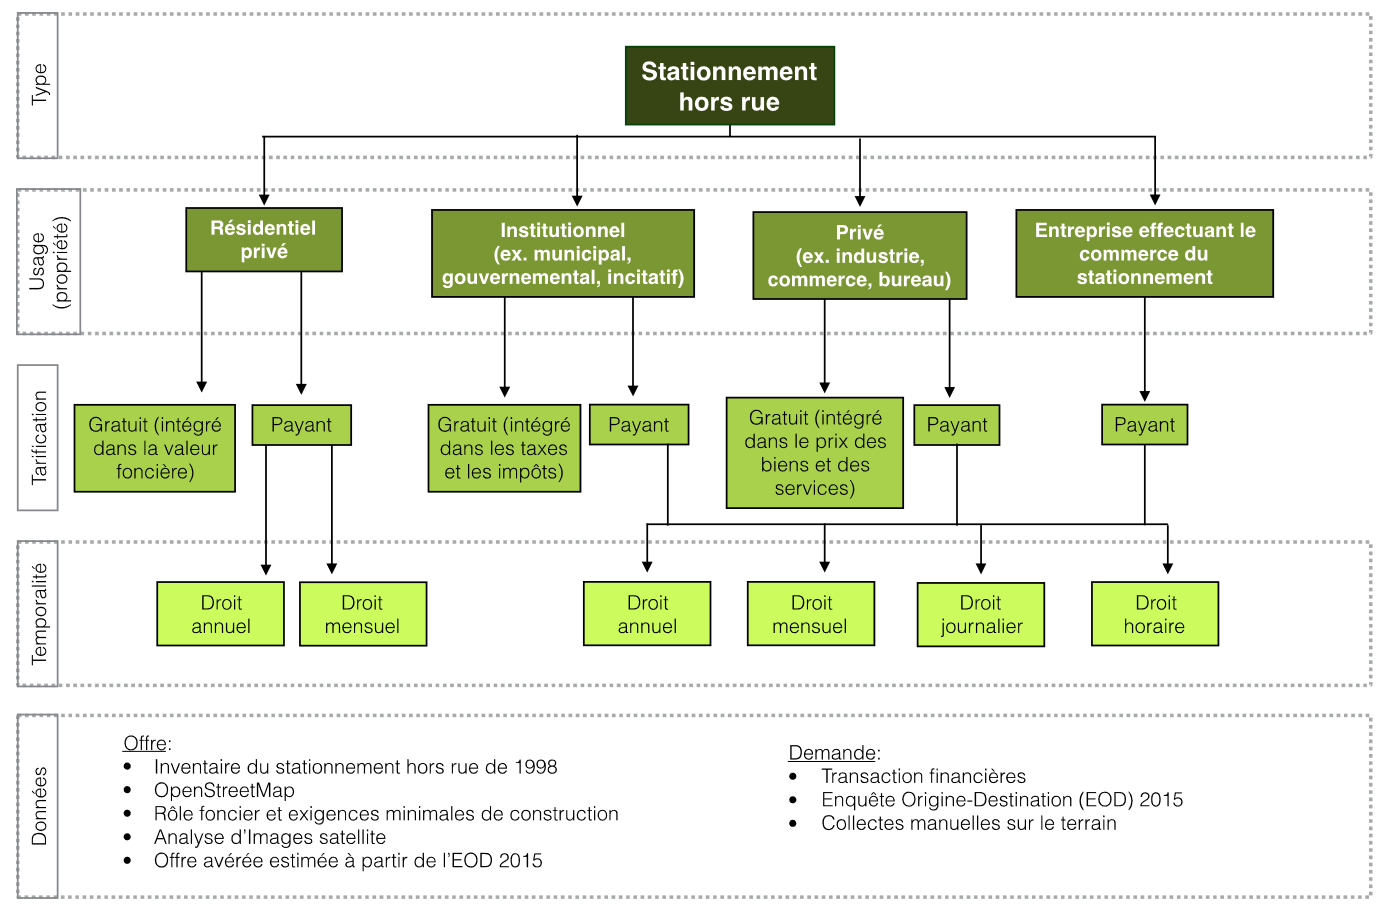
\includegraphics[width=1.0\textwidth]{images/Typologie_Stationnement_hors_rue.png}
      \caption{Typologie de stationnement hors rue. \hl{vérifier droits auteurs} Source: \cite{Morency:StationnementDans:2017}}
      \label{fig:Typo_Stat_hors_rue}
  \end{figure}
  \begin{figure}[ht]
      \centering
      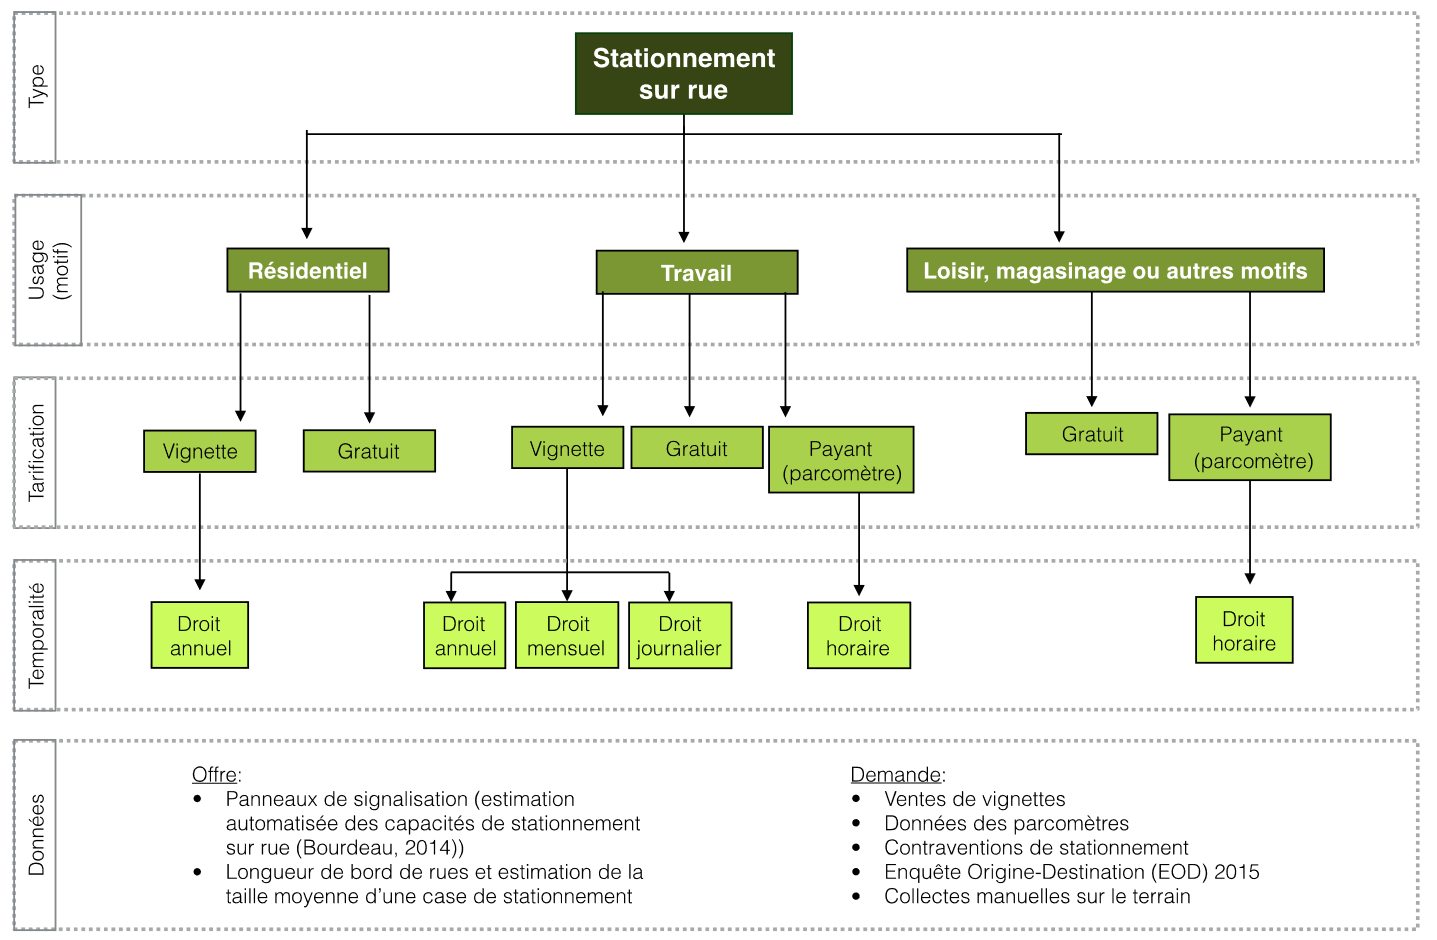
\includegraphics[width=1.0\textwidth]{images/Typologie_Stationnement_sur_rue.png}
      \caption{Typologie de stationnement sur rue. \hl{vérifier droits auteurs} Source: \cite{Morency:StationnementDans:2017}}
      \label{fig:Typo_Stat_sur_rue}
  \end{figure}
  Il est important de noter qu'il n'existe pas à la connaissance de l'auteur un inventaire tel que celui complété par le ministère des Transports pour la ville de Montréal \parencite{ConsortiumCIMA+-DanielArbouretassocies:InventaireEspaces:1998}. D'autre part, cet inventaire n'est pas mis à jour régulièrement et n'est donc pas particulièrement utile pour la mise à jour de plans de transports.  % Revue de littérature / Literature review

  


\section{Stationnement: politiques, couts et effets sur la mobilité}
  \subsection{Stationnement hors rue}
  Selon \textcite{Shoup:HighCost:2005}, les minimums de stationnement ont vu le jour dans les années 50 en réponse à la croissance du parc automobile et pour assurer que les commerçants et citoyens internalisaient les coûts associés à l'automobile. Ce mécanisme règlementaire est encore omniprésent au Québec puisque seuls les arrondissement de Côte des Neiges, du Sud-Ouest, du Plateau Mont-Royal et du Centre-Ville de Montréal \hl{besoin de citations}. 
  \subsection{Coûts de provision}
    Plusieurs coûts sont associés à la provision de stationnements, autant pour les individus, que pour les collectivités locales ou de tierces parties plus difficiles à identifier dans le cas d'externalités. Cette section visera à identifier quels sont les coûts associés et qui les porte.

    \subsubsection{Propriétaires fonciers et municipalités}
      \textcite{Blanc:EffectsUrban:2014} ont estimé la valeur foncière de 6 villes américaines en évaluant la valeur foncière des bâtiments et des stationnements extérieurs. En comparant le tissu urbain entre 1950 et 2010, les auteurs ont estimé la différence de valeur foncière et de revenu entre les deux configurations. Dans certains, les municipalités avaient accepté de détruire leur centre-ville pour permettre le développement de tours à bureaux entourées de stationnements. Dans d'autres, les municipalités avaient largement conservé le tissu urbain d'avant guerre. Dans tous les cas, le revenu foncier associé au stationnement était entre 5 et 10x moindre que le revenu associé aux bâtiments. L'étude est cependant associative puisqu'il est difficile d'isoler la nature causale entre la dilution du revenu foncier et la provision de stationnements, mais illustre les coûts d'opportunité associés à l'entreposage de véhicules personnels. \par

  \subsection{Effet de l'offre de stationnement sur la mobilité}
    \textcite{Chester:ParkingInfrastructure:2015} constatent que la capacité de stationnement est la plus haute dans le centre de la ville, mais que la croissance du parc de stationnement a principalement lieu sur le périmètre de la région.  Ils constatent aussi que le parc de stationnement a cru plus vite que la capacité routière, mais a suivi l'offre de stationnement résidentielle.\par
    \textcite{Guo:DoesResidential:2013} créé un modèle logit imbriqué pour identifier l'effet de l'offre de stationnement sur la motorisation des ménages de l'enquête OD de New York et trouve que la disponibilité de stationnement dans l'entrée et en bord de rue est potentiellement un plus grand déterminant de la motorisation qu'un garage. L'auteur suggère aussi que les programmes de vignette ont potentiellement des conséquences inattendues où la réduction de l'achalandage des stationnements par les non-résidents mène à une motorisation accrue des résidents, éliminant l'effet bénéfique de la réduction de l'offre des non-résidents. D'autre part, l'auteur trouve que la présence de nettoyage de rue réduit l'utilité marginale d'un véhicule supplémentaire et réduit la motorisation. Ces constats sont cependant limités au contexte de New York qui est une ville relativement dense avec une bonne desserte de transport en commun.\par
    \textcite{Yin:BuiltEnvironment:2018} associent eux aussi de manière significative la disponibilité du stationnement aux deux extrémités des déplacements à la possession et l'utilisation accrue d'automobile quoique la formulation des résultats rend difficile l'interprétation de la taille de l'effet.\par
    \textcite{Weinberger:ResidentialOffStreet:2009} font une analyse comparative entre Jackson Heights et Park Slope à New York. Jackson Heights a une part modale en auto-solo vers le centre-ville qui ne suit pas les principaux indicateurs de la motorisation (le revenu du ménage et la densité) et qui n'est pas expliqué par la desserte en \ac{TC} des deux quartiers. Les auteurs estiment l'offre de stationnement au travers du registre \ac{PLUTO} pour les bâtiments de 4 logements et plus ainsi qu'un échantillonnage pour les bâtiments comportant moins de 4 logements. Les auteurs ont constaté que Jackson Heights a 156\% plus d'offre de stationnement. Malgré le fait que Park Slope ait 46\% plus de stationnements en structure et en surface hors résidence, Jackson Heights a quatre fois plus d'espaces de stationnements privatifs dans les résidences. Les auteurs établissent ensuite des prospectives pour le développement résidentiel planifié par la ville et estiment que les résidents de ces nouveaux développements auront entre 42 et 49\% plus de chance d'être motorisés que les habitants actuels du fait des requis de stationnements minimums actuellement en effet. Bien que l'étude ne soit pas très robuste statistiquement, les auteurs concluent que les requis de stationnement minimum ne sont pas une bonne politique puisqu'ils effritent la qualité de l'environnement pour les marcheurs et augmentent l'attractivité de la possession d'une automobile. Les auteurs encouragent une étude systématique des liens entre la provision de stationnements, la motorisation et le choix modal.\par
    Deux études dans le contexte norvégien \parencite{Christiansen:ParkingFacilities:2017,Christiansen:HouseholdParking:2017} créent des modèles associatifs à partir d'enquêtes origine destination nationales. \textcite{Christiansen:ParkingFacilities:2017} trouvent que la limitation de la capacité de stationnement au travail avec une tarification est le moyen le plus efficace pour réduire la part modale de l'automobile pour ce type de trajet. Une tarification horaire ou journalière est aussi plus efficace pour réduire les trajets automobiles puisque le coût marginal pour chaque utilisation du stationnement est perçu par l'utilisateur. D'autre part, les auteurs trouvent que la proximité du stationnement au lieu d'habitation dans les milieux denses avec beaucoup d'offres de service à proximité. Les auteurs indiquent cependant qu'il y a des risques d'autosélection et d'endogénéité avec leur étude, un problème récurrent avec les études reliées au stationnement \parencite{Inci:ReviewEconomics:2015}. \textcite{Christiansen:HouseholdParking:2017} comparent les comportements de mobilité pour différents degrés d'accès au stationnement à la résidence. Ils trouvent qu'une distance d'accès supérieure à 50m a un effet marqué sur le choix modal sans affecter le nombre de trajets. Les trajets non contraints voient une plus grande différence de choix modal que les trajets motif travail. D'autre part, ils constatent peu de différence dans les taux de mobilité entre les ménages motorisés et non-motorisés, inférant que les dispositions de stationnement et de motorisation ont peu d'effet sur le bien-être. Les auteurs concluent qu'une gestion intégrée du stationnement qui inclut une combinaison d'une tarification 24/7 de règlements qui séparent le stationnement du logement physiquement et juridiquement et une gestion du nombre total de places de stationnement sont des leviers utiles pour gérer la demande de transport. Ils constatent le manque de lien causal dans leur étude, qui bien que non nécessaire pour l'établissement de politique efficace, est regrettable d'un point de vue scientifique.\par 
    Dans le contexte chinois, \textcite{Yin:BuiltEnvironment:2018} dressent des constats similaires à \textcite{Christiansen:HouseholdParking:2017} et \textcite{Christiansen:ParkingFacilities:2017} quant à l'influence de la disponibilité du stationnement à l'origine et la destination d'un trajet, même en contrôlant pour l'utilisation du territoire et les variables sociodémographiques, mais utilisent seulement des mesures agrégées de disponibilité totale de stationnement.\par
    \textcite{Currans:HouseholdsConstrained:2023} crée un modèle de régression et une analyse de médiation pour lier l'effet de l'offre de stationnement résidentiel hors rue avec la motorisation et les kilomètres parcourus par ménage et constatent que les ménages ayant des contraintes de stationnement (moins d'un stationnement par unité) parcourent moins de 10-23\% moins de kilomètres à typologie de voisinage constante. Les auteurs encouragent la présence de plus de questions sur les conditions de stationnement dans les enquêtes ainsi qu'à la création d'un inventaire de stationnement. \par
    \textcite{McCahill:EffectsParking:2016} observe la relation entre la provision de stationnements avec la part modale de l'automobile sous le prisme du critère de Bradford-Hill pour inférer que la provision de stationnements est la cause probable de l'augmentation de la part modale de l'automobile. \hl{cet article est intéressant mais le critère est très sujet à interprétation}

  \subsection{Allocation, tarification et ratissage}
    Une littérature économique riche existe sur les différents mécanismes d'allocation de places de stationnement qui est résumée par \textcite{Inci:ReviewEconomics:2015}, sur laquelle est largement basée cette section. Dès les premiers pas de la discipline, dans les années 50, la mise en place d'une tarification sur les infrastructures routières, variable dans le temps et l'espace, est identifiée comme une condition nécessaire pour réduire les externalités reliées au ratissage, la congestion et les externalités liées au transport urbain de personnes \parencite{Vickrey:StatementJoint:1994}. Les tentatives les plus intéressantes d'instaurer un marché variable viennent de San Francisco et Seattle où des projets pilotes ont été implémentés. Les études portant sur ces deux pilotes ont trouvé que la demande est initiallement inélastique, mais que le maintien de la politique amène des améliorations sur la disponibilité à long terme. \textcite{Chatman:TheoryImplementation:2014} constatent que l'implémentation de SFPark, le programme de tarification variable de San Francisco, ont eu des résultats mitigés. Bien que le taux d'occupation moyen, qui était l'indicateur utilisé pour faire varier la tarification,  ait été réduit à environ 80\%, le taux de disponibilité (le pourcentage de temps où au moins une place est disponible sur un tronçon) n'était pas sensible au prix avec les modalités politiques, l'imposition de prix plafond, la lenteur de l'adaptation du prix et le choix d'indicateur pour la tarification sont déterminants pour réduire les externalités liées à la recherche de stationnement. Cela amène un questionnement plus large sur la viabilité politique d'un système de tarification.\par
    \textcite{vanOmmeren:RealPrice:2011} infèrent la propension à payer pour un stationnement des résidents d'Amsterdam en utilisant les préférences révélées par le choix d'achat de résidence. En utilisant des données de ventes de résidences et en capitalisant la différence de prix sur le temps d'attente pour un permis de stationnement résident, les auteurs estiment une propension à payer de 10€ par jour, bien au-dessus du prix réel de 0.40€ et bien en dessous des recettes possibles pour les places tarifées aux visiteurs qui paient 2.3€ par heure.\par
    \textcite{Inci:ReviewEconomics:2015} mentionne les éléments suivants comme manquants à la recherche: l'effet de la prévention de la fraude, l'économie politique du stationnement, les interactions entre véhicules stationnés et en mouvement et l'établissement de l'élasticité de la demande dans plusieurs contextes spacio-temporels. Il est intéressant de noter qu'aucune mention n'est fait des coûts d'opportunités infligés aux autres modes ou activités par le stationnement dans la revue économique.

  \subsection{Utilisation de la capacité existante}
    \textcite{Translink:2018Regional:2019} a sondé les taux d'occupation des blocs-appartements et du stationnement sur rue dans la grande région de Vancouver. Pour l'échantillon donné, entre 30 et 40\% de la capacité de stationnement n'était pas utilisée. L'étude constate aussi que la demande de stationnement est plus faible chez les locataires que les propriétaires. Cela étant dit, l'étude ne recale pas les résultats sur l'ensemble du parc immobilier et n'utilise pas de test statistique pour valider la significativité de leurs résultats. La conception de l'étude n'a pas permis de quantifier les interactions entre le stationnement hors rue et sur rue pour les blocs appartements, mais indique qu'anecdotiquement, les praticiens ont constaté que les résidents utilisaient le stationnement sur rue plutôt qu'en sous-sol lorqu'il n'y avait pas de restriction sur le stationnement sur rue. 

  \subsection{Stationnement et utilisation du territoire}
    \textcite{Chester:ParkingInfrastructure:2015} trouvent que 16\% de la région est utilisée pour le stationnement, plus que l'ensemble du réseau routier. D'autre part, le centre-ville a vu une forte croissance de stationnements en structure et sous-terrains où les valeurs de terrains sont hautes. Les auteurs concluent qu'il y a 3.3 places de stationnement par véhicule et que la majorité de la croissance du parc de stationnement a eu lieu entre 1950 et 1980.\par
    \textcite{Davis:EstimatingParking:2010} estiment que 4.97\% de l'espace urbain est utilisé par le stationnement hors rue commerciale (sans compter les stationnements sur rue ou résidentiels). Ils estiment environ 1.8 places par voiture, 5.3 places par ménage et 1.7 places par adultes. À noter que l'indicateur ne mesure pas la même chose que \textcite{Chester:ParkingInfrastructure:2015} puisque ce dernier inclut les stationnements sur rue et résidentiel.

\section{Méthodes d'inventaire basées sur des données géoréférencées}
  La revue de littérature a révélé plusieurs différentes méthodologies utilisées pour recenser l'offre de stationnement hors rue et sur rue. 

  \subsection{Hors-Rue}
  \textcite{Chester:ParkingInfrastructure:2015} utilisent des données basées sur le rôle foncier, un modèle de croissance de la construction et des données de recensement croisées avec les minimums de stationnement issus des codes d'urbanisme pour inférer la capacité de stationnement de la région de Los Angeles depuis les années '50. Les auteurs indiquent qu'ils estiment que les minimums mis en place sont probablement le nombre de places construites du fait de la valeur marginale basse de la place de stationnement par rapport à la construction de bâtiments. \citeauthor{Chester:InventoryingSan:2022} estime la capacité de stationnement en utilisant une méthode similaire basée sur les codes d'urbanismes et les données foncières pour la région de San Francisco \parencite{Chester:InventoryingSan:2022} et Phoenix \parencite{Hoehne:ValleySundrenched:2019}. \textcite{Scharnhorst:QuantifiedParking:2018} fait pour sa part un inventaire de 5 régions métropolitaines aux États-Unis utilisant encore une fois des méthodes basées sur les codes d'urbanisme en vigueur à la période de construction. Ce dernier n'est cependant pas revu par les pairs. \par 
  Il est important de noter que ce type d'inventaire fait l'hypothèse que les promoteurs immobiliers construisent le minimum de places possibles. \textcite{Stangl:ParkingLots:2019} indique que les promoteurs immobiliers ne respectent pas nécessairement cette hypothèse car leur but est de minimiser les risques d'invendus et leurs perceptions ne sont pas alignées avec l'utilisation réelle des stationnements. Ironiquement, les développeurs ont tendance à bâtir plus de stationnements dans des voisinages de typologie \og{Old Urban} \fg{} \parencite{Voulgaris:SynergisticNeighborhood:2017} alors que ce sont précisément les quartiers où les gens ont une plus faible propension à conduire. \textcite{Stangl:ParkingLots:2019} comporte des entrevues avec des promoteurs immobiliers qui illustrent l'effet structurant des minimums de stationnement sur les décisions de construction, mais aussi certains biais dans la prise de décision vis-a-vis du stationnement.

  \subsection{Sur-rue}
  \textcite{Bourdeau:MethodologieAnalyse:2014} détaille une méthode d'inventaire de places de stationnement sur rue basé sur l'utilisation des données de bords de réseau routiers, de panneaux de stationnement et d'archive cadastrale indiquant les entrées charretières pour déterminer le nombre de places de stationnements sur rue. Cette approche permet de mieux identifier les limites règlementaires et temporelles que les approches utilisées par \textcite{Chester:InventoryingSan:2022} et \textcite{Scharnhorst:QuantifiedParking:2018}. En effet, ces dernières n'enlèvent de la capacité que sur une base de moyennes pour les intersections, arrêts de bus sans prendre en compte la géométrie locale ou des contraintes qui ne peuvent être adéquatement capturées par \ac{OSM}. Dans les 2 cas ci-haut, l'inventaire sur rue est fait avec des largeurs d'intersection moyenne, avec des retraits pour les entrées et la règlementation utilisant des heuristiques plutôt que la réalité du terrain. \par
\section{Méthodes d'inventaire basées sur l'imagerie aérienne sans apprentissage machine}
  \textcite{Akbari:AnalyzingLand:2003} utilisent des orthophotos en couleur avec une résolution de 0.3m pour identifier le pourcentage d'utilisation des sols de différentes surfaces (bâtiments, verdure, stationnements, etc.). Une approche de Monte-Carlo est utilisée où un sous-ensemble de pixels se voit assigner une utilisation des sols manuellement pour chaque sous-ensemble de photos basé principalement sur la couleur du pixel. Le nombre de pixels manuellement identifié est validé contre la convergence du pourcentage d'utilisation des sols jusqu'à un seuil de 1\%. Une fois ce sous-ensemble identifié, l'utilisation des sols est assignée à l'ensemble des pixels de l'orthophoto. \citeauthor{Akbari:AnalyzingLand:2003} ne font pas de distinction entre la voirie et le stationnement sur rue.\par
  \textcite{Davis:EstimatingParking:2010} recensent un sous ensemble de codes postaux manuellement avant d'utiliser une régression pour estimer le stationnement sur l'ensemble d'un territoire. Une régression basée sur une codification d'\og{urbanité} \fg{} des codes postaux issue du recensement est ensuite utilisée pour inférer l'offre de stationnement hors rue non résidentielle sur un territoire s'étendant sur 4 états dans le Midwest des États-Unis. La méthode est validée sur un sous-ensemble de données qui n'est pas utilisé pour la régression et les auteurs constatent une erreur de 5\% entre la valeur inférée par régression et la valeur mesurée manuellement pour le sous-ensemble de contrôle. Comme l'étude précédente, cette étude n'inclut que le stationnement hors rue. \par
\section{Méthodes d'inventaire basées sur l'imagerie aérienne et l'apprentissage machine}
  L'augmentation de la capacité de calcul numérique et la démocratisation des méthodes d'apprentissage machine a mené \textcite{Hellekes:ParkingSpace:2023} à utiliser la photographie aérienne et des données \ac{OSM} pour identifier les aires de stationnement à l'aide d'une méthode Dense-U-Net. D'autre part, les auteurs utilisent plusieurs ensembles d'orthophotos d'une même zone et les données \ac{OSM} pour identifier les zones de stationnement non démarquées, intermittentes ou informelles comme les trottoirs et jardins. Des méthodes de régression Bayesienne sont utilisées pour introduire explicitement l'incertitude dans la reconnaissance de l'objet de stationnement. \textcite{Henry:CitywideEstimation:2021} est un autre article par la même équipe de recherche qui donne un aperçu des différentes méthodes d'apprentissage machine utilisées jusqu'à présent pour identifier des objets dans un périmètre urbain. D'autre part, ils indiquent que la méthodologie de fusion choisie influe sur les résultats en fonction du type d'objet reconnu. Par exemple, l'inclusion des données \ac{OSM} améliore l'identification de routes et de voies d'accès, mais nuit à l'identification de stationnement.  \par
  \textcite{Yin:ContextenrichedSatellite:2022} est un autre article portant sur l'inventaire de stationnement en utilisant des méthodes d'apprentissage machine pour détecter des stationnements. En plus d'utiliser l'imagerie satellite, les auteurs utilisent des données \ac{OSM} pour ajouter du contexte et voient une amélioration la métrique de de détection \ac{IoU} d'environ 2.5\% en ajouant 2 dimensions supplémentaires au tenseur d'images. Les auteurs on en effet pris les couches de bâtiments et de routes d'\ac{OSM} pour donner plus de contexte aux algorithmes d'aprrentissage machines. Les éléments OSM ont généré 15 dimensions supplémentaires au tenseur qui ont été réduit à 3 par convolution et avec une activation en utilisant une fonction tanh. Ce résultat est ensuite additionné au 3 dimensions d'une image RGB. Ils ont par la suite étalloné leur méthode avec plusieurs algorithmes de segmentation d'image: U-Net, U-Net++, LinkNet, D-LinkNet, FPN, PAN, DeepLab v3 et Deeplab v3+. Les algorithmes ont été testés avec et sans contexte et les auteurs constatent que l'algorithme DeepLab v3 performe le mieux particulièrement sur les stationnement de plus petite taille.
\section{Apprentissage machine}
  \subsection{Principe de base}
    Selon l'\ac{OQLF}\parencite{oqlf_apprentissage_2024}, la définition de l'apprentissage profond est la suivante:
    \begin{definition}
    Mode d'apprentissage automatique généralement effectué par un réseau de neurones artificiels composé de plusieurs couches de neurones hiérarchisées selon le degré de complexité des concepts, et qui, en interagissant entre elles, permettent à un agent d'apprendre progressivement et efficacement à partir de mégadonnées.
    \end{definition}
    D'un point de vue mathématique, l'apprentissage est obtenu en représentant les données sous forme matricielle ou vectorielles et en les soummettant à plusieurs opérations algébriques simples successivement de manière à ce que le code produise une sortie désirée. Le problème est formulé non pas en demandant à ce que le logiciel performe des opérations spécifiques, mais en spécifiant une architecture de réseau et un ensemble de pondérations à modifier pour minimiser une fonction de perte donnée.
  \subsection{Le pipeline d'apprentissage machine}
  \subsubsection{Survol}
      Cette section va décrire le processus utilisé pour obtenir des résultats dans le champs de l'apprentissage machine. Ce processus est souvent appelé \og{pipeline d'apprentissage machine} \fg{}. Il est décliné en 6 étapes:
        \begin{enumerate}
          \item Préparation des données
          \item Ingénierie des caractéristiques
          \item Développement du réseau et entrainement
          \item Évaluation des résultats et amélioration du modèle
          \item Déploiement et suivi
        \end{enumerate}
      Les sections suivantes détailleront les opérations à chaque étape
    \subsubsection{Collection et préparation des données}
        La préparation des données consiste à prendre un ensemble de données et au besoin le nettoyer, enlever les données abérantes, de mettre à l'échelle les données et la création d'un ensemble de données d'apprentissage et d'un ensemble de validation.
    \subsubsection{Ingénierie des caractéristiques}
      L'ingénierie des caractéristiques consiste à créer des variables intermédiaires, catégoriques ou de traiter les données de manière à améliorer la capacité prédicitive du modèle d'apprentissage machine dans l'extraction des données pertinentes.
    \subsubsection{Sélection, codage et entrainement du modèle}
      Cette partie du \og{pipeline} \fg{} est le coeur de l'opération. À cette étape, une méthode d'extraction des données est choisie et implémentée. Le modèle peut être un modèle personalisé, issu de la littérature ou d'une librairie pré construite. Deux méthodes sont potentiellement applicables à l'apprentissage. Un modèle pré-existant, avec ses pondérations, peut être appliqué à un nouveau problème en utilisant de l'apprentissage de transfert (\og{Transfer Learning} \fg{} en anglais) ou le modèle peut être entrainé à partir de pondérations initiales aléatoires. L'apprentissage itère au travers de l'ensemble de données en mettant les données en lots (\og{Batch} \fg{} en anglais) et en modifiant les pondération de manière à minimiser la fonction de pertes. À chaque fois que le modèle complète une itération au travers de l'ensemble des données, une époque (\og{epoch} \fg{} en anglais) est dite complétée. La plupart du temps, la fonction de perte utilisée est compilée pour l'ensemble d'entrainement et de validation à la fin de chaque époque pour permettre d'évaluer la convergence du modèle, ainsi que le degré de sur-ajustement potentiel du modèle. Un modèle est dit sur-ajusté s'il prédit bien sur l'ensemble d'appentissage mais mal sur l'ensemble de validation. Dans certains, la vitesse de prédiction où la taille des modèles peut-être un facteur limitant si le modèle doit être implémentée sur un appareil mobile ou sur des applications temps réel.
    \subsubsection{Évaluation du modèle}
      Une fois l'apprentissage completé, le modèle peut-être évalué de différentes manières. Plusieurs indicateurs mesurent le degré de précision du modèle, la vitesse de sa convergence peuvent être évalués en fonction de l'utilisation désirée du modèle. En vision numérique, le degré de similarité entre les données d'apprentissage annotées et les prédictions est souvent la métrique d'évaluation de prédilection.
    \subsubsection{Déploiement et suivi}
      À cette étape, le modèle est deployé. Le suivi consiste principalement à recenser les comportements abhérants du modèle et à les réintégrer dans le modèle au besoin. 
  \subsection{Principe de base des réseaux de neurones}
  Le principe de base des réseaux de neurones et qu'en implémentant de multiples couches de fonctions linéaires couplées avec des fonctions d'activation, il est possible de reproduire des tâches ou fonctions complexes. 
    \subsubsection{Le neurone}
      Chaque neurone dans un réseau est une opération algébrique avec une fonction d'activation:

        \begin{figure}[!h]
          \centering
          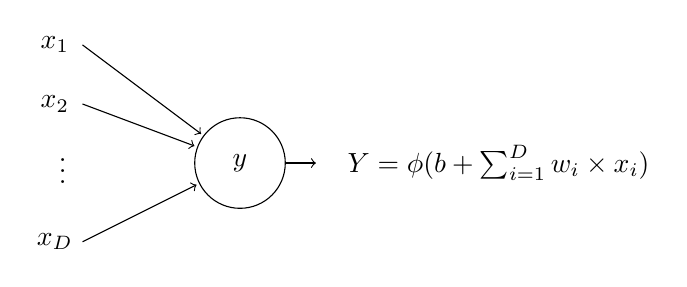
\begin{tikzpicture}[shorten >=1pt,->]
            \tikzstyle{unit}=[draw,shape=circle,minimum size=1.15cm]
            \node[unit](p) at (2,1){$y$};
            \node(dots) at (-0.25,1){\vdots};
            \draw (0,2.5) node[xshift=-10]{$x_1$} --(p);
            \draw (0,1.75) node[xshift=-10]{$x_2$} --(p);
            \draw (0,0) node[xshift=-10]{$x_D$} -- (p);
            \draw (p) -- (3,1) node[xshift=65]{$Y = \phi(b  + \sum_{i=1}^{D} w_i \times x_i)$};
          \end{tikzpicture}
          \caption{Un neurone dans un réseau de neurone}
          \label{fig:neurone}
         % https://davidstutz.de/illustrating-convolutional-neural-networks-in-latex-with-tikz/
        \end{figure}
      La fonction $\phi $ est une fonction d'activation qui sera détaillée dans la section \ref{sssection:activ_fn}.
      \FloatBarrier
    \subsubsection{Réseau de neurones simple}
      Un réseau de neurones arrange plusieurs neurones en série ou en parallèle où les pondérations sont altérées pour permettre de faire des tâches variant en complexité. Une couche est un ensemble de neurones qui est le résultat d'un même nombre d'opérations algébriques. Les différentes couches peuvent avoir des nombres de neurones variables. La couche entrante est le premier ensemble de données qui est fourni au réseau et la couche sortante est la dernière couche de neurones en sortie à l'analyste. La figure \ref{fig:perceptron} montre une architecture hypothétique de réseau de neurones.\par
      \begin{figure}[!h]
        \centering
          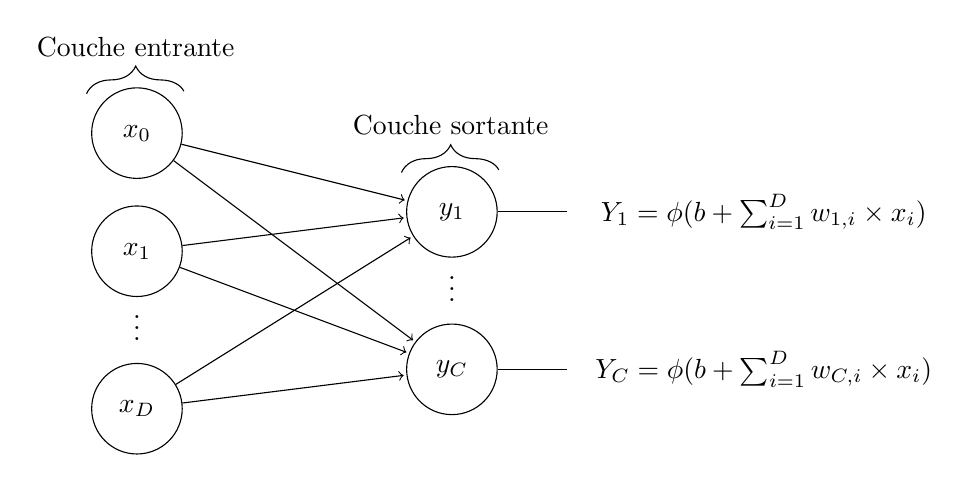
\begin{tikzpicture}[shorten >=1pt]
            \tikzstyle{unit}=[draw,shape=circle,minimum size=1.15cm]
    
            \node[unit](x0) at (0,3.5){$x_0$};
            \node[unit](x1) at (0,2){$x_1$};
            \node(dots) at (0,1.125){\vdots};
            \node[unit](xd) at (0,0){$x_D$};
    
            \node[unit](y1) at (4,2.5){$y_1$};
            \node(dots) at (4,1.625){\vdots};
            \node[unit](yc) at (4,0.5){$y_C$};
            \draw (y1) -- (5.5,2.5) node[xshift=70]{$Y_1 = \phi(b + \sum_{i=1}^{D} w_{1,i} \times x_i)$};
            \draw (yc) -- (5.5,0.5) node[xshift=70]{$Y_C = \phi(b + \sum_{i=1}^{D} w_{C,i} \times x_i)$};
    
            \draw[->] (x0) -- (y1);
            \draw[->] (x0) -- (yc);
    
            \draw[->] (x1) -- (y1);
            \draw[->] (x1) -- (yc);
    
            \draw[->] (xd) -- (y1);
            \draw[->] (xd) -- (yc);
    
            \draw [decorate,decoration={brace,amplitude=10pt},xshift=-4pt,yshift=0pt] (-0.5,4) -- (0.75,4) node [black,midway,yshift=+0.6cm]{Couche entrante};
            \draw [decorate,decoration={brace,amplitude=10pt},xshift=-4pt,yshift=0pt] (3.5,3) -- (4.75,3) node [black,midway,yshift=+0.6cm]{Couche sortante};
          \end{tikzpicture}
          % https://davidstutz.de/illustrating-convolutional-neural-networks-in-latex-with-tikz/
        \caption{Réseau de neurones à couche simple}
        \label{fig:perceptron}
      \end{figure}
      Le réseau montré à la figure \ref{fig:perceptron} est dit pleinement connecté si sa valeur est une somme pondérée de l'ensemble des couches précédentes. 
      \FloatBarrier
    \subsubsection{Réseau de neurones multicouches}
      Plusieurs couches dites \og{cachées} \fg{} peuvent être ajoutées entre l'entrée et la sortie du réseau de neurones pour permettre de traiter des problèmes plus ou moins complexes. L'enjeu comporte cependant des compromis puisque l'ajout de couches ajoute des paramètres à ajuster, augmentant la taille du modèle. D'autre part, plus le nombre de paramètres est grand, plus la contribution d'une pondération est petite. Ce problème est nommé le problème de \og{disparition de gradient} \fg{} dans la littérature.
      \begin{figure}[!h]
        \centering
          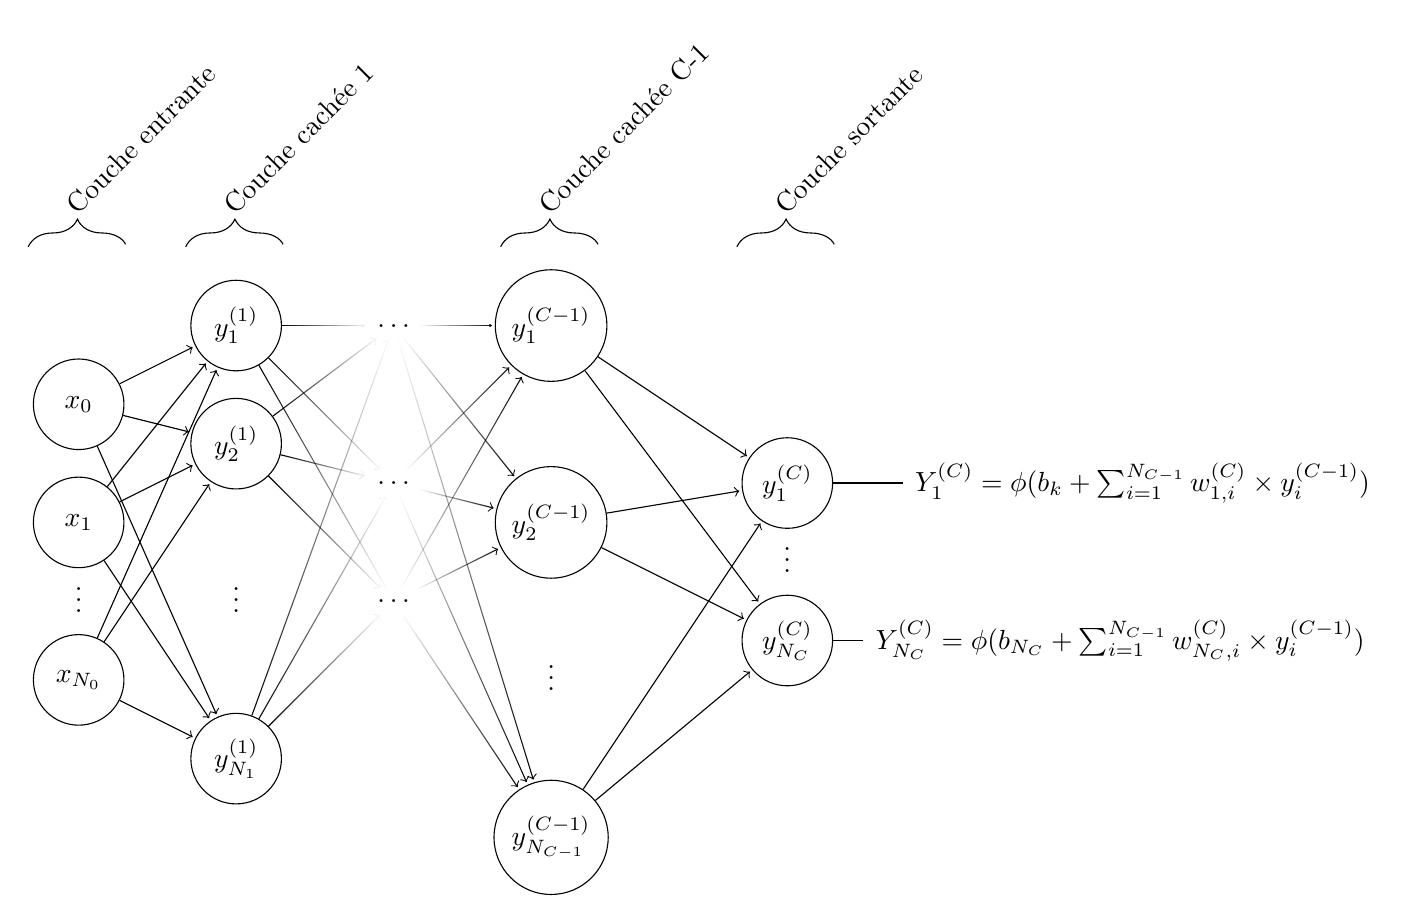
\begin{tikzpicture}[shorten >=1pt]
            \tikzstyle{unit}=[draw,shape=circle,minimum size=1.15cm]
    
            \node[unit](x00) at (-1,3.5){$x_0$};
            \node[unit](x01) at (-1,2){$x_1$};
            \node(dots) at (-1,1.125){\vdots};
            \node[unit](x0d) at (-1,0){$x_{N_0}$};

            \node[unit](y11) at (1,4.5){$y_1^{(1)}$};
            \node[unit](y12) at (1,3){$y_2^{(1)}$};
            \node(dots1) at (1,1.125){\vdots};
            \node[unit](y1n) at (1,-1){$y_{N_1}^{(1)}$};

            \node(middots1) at (3,4.5){$\ldots$};
            \node(middots2) at (3,2.5){$\ldots$};
            \node(middots3) at (3,1){$\ldots$};

            \node[unit](yc-11) at (5,4.5){$y_1^{(C-1)}$};
            \node[unit](yc-12) at (5,2){$y_2^{(C-1)}$};
            \node(dotsc) at (5,0.125){\vdots};
            \node[unit](yc-1n) at (5,-2){$y_{N_{C-1}}^{(C-1)}$};

            \node[unit](yc1) at (8,2.5){$y^{(C)}_1$};
            \node(dotsn) at (8,1.625){\vdots};
            \node[unit](ycn) at (8,0.5){$y^{(C)}_{N_{C}}$};
            \draw (yc1) -- (9.5,2.5) node[right]{$Y^{(C)}_{1} = \phi(b_k + \sum_{i=1}^{N_{C-1}} w^{(C)}_{1,i} \times y^{(C-1)}_i)$};
            \draw (ycn) -- (9,0.5) node[right]{$Y^{(C)}_{N_{C}} = \phi(b_{N_C} + \sum_{i=1}^{N_{C-1}} w^{(C)}_{N_{C},i} \times y^{(C-1)}_i)$};
    
            \draw[->] (x00) -- (y11);
            \draw[->] (x00) -- (y12);
            \draw[->] (x00) -- (y1n);
    
            \draw[->] (x01) -- (y11);
            \draw[->] (x01) -- (y12);
            \draw[->] (x01) -- (y1n);
    
            \draw[->] (x0d) -- (y11);
            \draw[->] (x0d) -- (y12);
            \draw[->] (x0d) -- (y1n);

            \draw[->,path fading=east] (y11) -- (middots1);
            \draw[->,path fading=east] (y12) -- (middots1);
            \draw[->,path fading=east] (y1n) -- (middots1);

            \draw[->,path fading=east] (y11) -- (middots2);
            \draw[->,path fading=east] (y12) -- (middots2);
            \draw[->,path fading=east] (y1n) -- (middots2);

            \draw[->,path fading=east] (y11) -- (middots3);
            \draw[->,path fading=east] (y12) -- (middots3);
            \draw[->,path fading=east] (y1n) -- (middots3);

            \draw[->,path fading=west] (middots1) -- (yc-11);
            \draw[->,path fading=west] (middots1) -- (yc-12);
            \draw[->,path fading=west] (middots1) -- (yc-1n);

            \draw[->,path fading=west] (middots2) -- (yc-11);
            \draw[->,path fading=west] (middots2) -- (yc-12);
            \draw[->,path fading=west] (middots2) -- (yc-1n);

            \draw[->,path fading=west] (middots3) -- (yc-11);
            \draw[->,path fading=west] (middots3) -- (yc-12);
            \draw[->,path fading=west] (middots3) -- (yc-1n);

            \draw[->] (yc-11) -- (yc1);
            \draw[->] (yc-11) -- (ycn);

            \draw[->] (yc-12) -- (yc1);
            \draw[->] (yc-12) -- (ycn);

            \draw[->] (yc-1n) -- (yc1);
            \draw[->] (yc-1n) -- (ycn);
    
            \draw [decorate,decoration={brace,amplitude=10pt},xshift=-4pt,yshift=0pt] (-1.5,5.5) -- (-0.25,5.5) node [black,right,xshift=-0.8cm,yshift=+0.4cm,rotate=45]{Couche entrante};
            \draw [decorate,decoration={brace,amplitude=10pt},xshift=-4pt,yshift=0pt] (0.5,5.5) -- (1.75,5.5) node [black,right,xshift=-0.8cm,yshift=+0.4cm,rotate=45]{Couche cachée 1};
            \draw [decorate,decoration={brace,amplitude=10pt},xshift=-4pt,yshift=0pt] (4.5,5.5) -- (5.75,5.5) node [black,right,xshift=-0.8cm,yshift=+0.4cm,rotate=45]{Couche cachée C-1};
            \draw [decorate,decoration={brace,amplitude=10pt},xshift=-4pt,yshift=0pt] (7.5,5.5) -- (8.75,5.5) node [black,right,xshift=-0.8cm,yshift=+0.4cm,rotate=45]{Couche sortante};
          \end{tikzpicture}
          % https://davidstutz.de/illustrating-convolutional-neural-networks-in-latex-with-tikz/
        \caption{Réseau de neurones à couches multiples}
        \label{fig:multi_layer_perceptron}
      \end{figure}
      \FloatBarrier
  \subsection{Opérations communes dans l'apprentissage machine}
    \subsubsection{La fonction de perte}
      La fonction de perte de perte est la fonction objectif que le réseau de neurones essaie de minimiser. \textcite{azad_loss_2023, jadon_survey_2020} donnent un survol des principaux types de fonction de pertes et de leur applicabilité pour différentes tâches de segmentation d'image. Le choix d'une fonction de perte est dépendant de la taille de l'objet à détecter et de l'équilibre entre les différentes classes à détecter:\par
      \paragraph{Entropie Croisée} L'entropie croisée est une mesure de la distance statistique entre deux ensembles et a été introduite par \textcite{shannon_mathematical_1948}. Ici elle mesure la distance entre la prédiction du modèle et les annotations sur les données entrantes. Pour donner une distribution de probabilité, une fonction softmax est appliquée aux résultantes du réseau de neurones.
      Les équations \ref{eq:entropie_croisee}, \ref{eq:grnd_truth_vector} et \ref{eq:prob_class_vector} donnent la définition formelle de l'entropie croisée \parencite{wallach_deep_2024}.\par
      \begin{align}
        EC & = -\frac{1}{I \times N} \sum_{n=1}^{N_{images}}\sum_{i=1}^{N_{pixels}}\sum_{j=1}^{N_{classes}}r^{n}_{ij} \log{p^{n}_{ij}} \label{eq:entropie_croisee}\\
        r^{n}_{ij} & = \begin{cases}
          1,& \mbox{si le pixel i de l'image n appartient à la classe j dans l'annotation d'entrainement}\\
          0,& \mbox{autrement}\\ \end{cases}\label{eq:grnd_truth_vector}\\
        p^{n}_{ij} & \in [0,1]\mbox{ est la prédiction du modèle concernant la catégorie j pour le pixel i}\label{eq:prob_class_vector}
      \end{align}
      $r^{n}_{ij}$ est la classe(j) annotée du pixel i de l'image n et $p^{n}_{ij}$ est la probabilité prédite par le modèle que le pixel i de l'image j appartienne à la classe j. La probabilité est obtenu en appliquant une fonction softmax aux sorties du modèle. 
      \paragraph{Entropie Croisée binaire} L'entropie croisée peut être utilisé pour un problème de classification binaire. Dans ce cas, il n'y a que 2 classes (vrai ou faux). L'entropie croisée binaire peut donc être représenté par les équations \ref{eq:entropie_croisee_binaire}, \ref{eq:grnd_truth_vector_ecb} et \ref{eq:prob_class_vector_ECB}
      \begin{align}
        ECB & = -\frac{1}{I \times N} \sum_{n=1}^{N_{images}}\sum_{i=1}^{N_{pixels}}r^{n}_{iV} \log{p^{n}_{iV}} +
        (1-r^{n}_{iV}) \log{(1-p^{n}_{iV})} \label{eq:entropie_croisee_binaire}\\
        r^{n}_{iV} & = \begin{cases}
          1,& \mbox{si le pixel i de l'image n appartient à la classe d'identification dans l'annotation d'entrainement}\\
          0,& \mbox{autrement}\\ \end{cases}\label{eq:grnd_truth_vector_ecb}\\
        p^{n}_{iV} & \in [0,1]\mbox{ est la probabilité que le pixel i appartienne à la classe identifiée}\label{eq:prob_class_vector_ECB}
      \end{align}
      \paragraph{Coefficient de Dice} 
      Le coefficient de Dice trouve ses origines dans les sciences de la nature \parencite{dice_measures_1945} et est défini aux équations \ref{eq:DICE1} et \ref{eq:DICE2}.
      \begin{align} 
        CDS & = \frac{2 \times \lvert X \cap Y \rvert}{\lvert X \rvert + \lvert Y \rvert}\label{eq:DICE1} \\
        CDS & = \frac{2 \times VP}{2 \times VP + FP + FN}\label{eq:DICE2}
      \end{align}
    \subsubsection{Métriques pour l'évaluation}
      \paragraph{Indice de Jaccard} L'indice de Jaccard provient lui aussi des sciences de la nature \parencite{jaccard_distribution_1901} et est plus communément utilisé comme fonction pour l'évaluation de différentes méthodes d'apprentissage. Il est très similaire au coefficient de Dice. L'indice de Jaccard est défini aux équations \ref{eq:IoU1} et \ref{eq:IoU2}. On réfère à cet indice sous le nom d'\ac{IoU} dans la plupart de la littérature. Il n'est pas utilisé comme fonction de perte puisqu'il n'est pas différentiable et ne se prête donc pas à la rétro-propagation.
      \begin{align} 
        IoU & = \frac{\lvert X \cap Y \rvert}{\lvert X \cup Y \rvert}\label{eq:IoU1} \\
        IoU & = \frac{VP}{VP + FP + FN}\label{eq:IoU2}
      \end{align}
      \paragraph{Justesse ou \og{Accuracy} \fg{}} 
      La justesse vise à quantifier le pourcentage de prédictions valides du modèle et est définie à l'équation \ref{eq:acc}\parencite{wallach_deep_2024}.
      \begin{align}
        Justesse & = \frac{VP+VN}{VP + FP + FP + FN}\label{eq:acc}
      \end{align}
      \paragraph{Précision}
      La précision indique quel pourcentage des zones identifiées est valide et est définie à l'équation \ref{eq:prec}\parencite{wallach_deep_2024}.
      \begin{align}
        Precision & = \frac{VP}{VP + FP}\label{eq:prec}
      \end{align}
      \paragraph{Rappel ou \og{Recall} \fg{}}
      La rappel indique quel pourcentage des zones positives n'ont pas été identifiées. Il est défini à l'équation \ref{eq:rappel}\parencite{wallach_deep_2024}.
      \begin{align}
        Rappel & = \frac{VP}{VP + FN}\label{eq:rappel}
      \end{align}
      \paragraph{Score F1} Le Score F1 indique la capacité du modèle à faire un compromis entre la précision des prédictions et la capacité à ne pas manquer d'instances. Il est défini à l'équation 
      \begin{align}
        F1 & = \frac{2}{\frac{1}{Rappel} + \frac{1}{Precision}}\label{eq:F1_1}\\
        F1 & = \frac{VP}{VP + \frac{1}{2} (FN + FP)}
      \end{align}
    \subsubsection{Apprentissage et Rétro-propagation}
      La rétro-propagation a été introduite comme méthode pour modifier les pondérations des différents opérations algébriques par \textcite{rumelhart_learning_1986}. La méthode consiste à créer une fonction cumulée d'erreur pour les extrants des réseaux neuronaux. Ensuite, des dérivées partielles sont calculées pour chaque neurones en amont pour trouver la modification requises pour minimiser la fonction d'erreur. Deux méthodes sont envisagées dans l'article initial. La première, modifie les pondérations après chaque donnée d'entrainement tandis que la deuxième somme les erreurs pour l'ensemble du jeu de données d'entrainement. Une troisième voie existe et est le plus souvent exploitée aujourd'hui qui consiste à calculer les modifications aux pondérations pour des lots de données qui sont des sous-ensemble de l'échantillon complet. En effet, le calcul des pondérations pour chaque échantillon créé des problèmes de stabilité et de convergence pour l'algorithme puisqu'un échantillons peut être à la limite de l'ensemble et créer un grande variation de paramètre mais l'évaluation des dérivées pour l'ensemble de l'échantillon peut être trop honéreux en termes de mémoire pour de grands échantillons \parencite{wallach_deep_2024}.\par
      
      Soit une fonction d'erreur E, et le neurone $ y^{(C)}_1 $ de la figure \ref{fig:multi_layer_perceptron}. Il est possible trouver les variations de pondérations qui réduiraient l'erreur par l'équation \ref{eq:deriv_weights} comme le montre \textcite{rumelhart_learning_1986}:
      \begin{align}
        x^{C}_k &= b_k + \sum_{i=1}^{N_{C-1}} w^{(C)}_{k,i} \times Y^{(C-1)}_i\\
        Y^{C}_k &= \phi(x^{C}_k)\\
        E &= \sum^{N_C}_{k=1} f(Y^{C}_k)\\
        \frac{\partial{E}}{\partial{w^{(C)}_{k,i}}}\bigg|_{w=\overrightarrow{w}_{t}} &= \frac{\partial{E}}{\partial{f(Y^{C}_k)}} \cdot \frac{\partial{f(Y^{C}_k)}}{\partial{w^{(C)}_{k,i}}}\\
        \frac{\partial{E}}{\partial{w^{(C)}_{k,i}}}\bigg|_{w=\overrightarrow{w}_{t}} &= \frac{\partial{E}}{\partial{f(Y^{C}_k)}} \cdot \frac{\partial{f(Y^{C}_k)}}{\partial{Y^{C}_k}} \cdot \frac{\partial{Y^{C}_k}}{\partial{w^{(C)}_{k,i}}} \\
        \frac{\partial{E}}{\partial{w^{(C)}_{k,i}}}\bigg|_{w=\overrightarrow{w}_{t}} &= \frac{\partial{E}}{\partial{f(Y^{C}_k)}} \cdot \frac{\partial{f(Y^{C}_k)}}{\partial{Y^{C}_k}} \cdot \frac{\partial{Y^{C}_k}}{\partial{x^{C}_k}} \cdot \frac{\partial{x^{C}_k}}{\partial{w^{(C)}_{k,i}}}\\
        \underbrace{\frac{\partial{E}}{\partial{w^{(C)}_{k,i}}}\bigg|_{w=\overrightarrow{w}_{t}}}_\text{Perte / poids} &= \underbrace{\frac{\partial{E}}{\partial{f(Y^{C}_k)}}}_\text{Perte / fn perte} \cdot \underbrace{\frac{\partial{f(Y^{C}_k)}}{\partial{Y^{C}_k}}}_\text{Fn perte / sortie activation} \cdot \underbrace{\frac{\partial{Y^{C}_k}}{\partial{x^{C}_k}}}_\text{Activation / fn lin.} \cdot \underbrace{Y^{(C-1)}_i}_\text{fn lin. / pond.}\label{eq:deriv_weights}
      \end{align}
    Dans son implémentation la plus simple, un vecteur de l'ensemble des dérivées partielles $\nabla{w_{t}} = \left[ \frac{\partial{E}}{\partial{w^{(1)}_{1,1}}} \ldots \frac{\partial{E}}{\partial{w^{(C)}_{k,i}}} \right] $ est multiplié par un paramètre fixe et ajouté aux paramètres actuels $\overrightarrow{w}_{t} = \left[w^{(1)}_{1,1} \ldots w^{(C)}_{k,i}  \right] $. Les pondérations pour la prochaine itération donc $\overrightarrow{w}_{t+1} = \overrightarrow{w}_{t} - \varepsilon \cdot \nabla{w_{t}} $. Dans les méthodes modernes, des paramètres d'inertie et de vitesses sont ajoutés pour améliorer la stabilité des algorithmes. La section \ref{ssec:grad_desc} détaillera les algorithmes de descente de gradient les plus communs. Il est important de noter que ces méthodes n'utilisent pas des méthodes de second ordre(par exemple l'algorithme de Newton-Raphson) pour limiter le temps de calcul 
    \subsubsection{Fonctions d'activation}\label{sssection:activ_fn}
    La fonction d'activation a pour but de rendre la sortie de la convolution non-linéaire. Cette non-linéarisation facilite la détection de lieux d'intérêt en créant une démarcation claire entre les zones où il y a un fort potentiel d'activation et où il n'y en a pas. 3 fonctions sont typiquement utilisées à cette fin: 
      \begin{itemize}
        \item une fonction sigmoide utilsée dans les fonctions logistique pour assurer une frontière entre 1 et zéro $f(x) = 1/1+ e^{-x} $
        \item une fonction de tangente hyperbolique $f(x) = \tanh(x) $ 
        \item une fonction de \ac{ReLu} qui est $f(x)  = max(0,x) $
      \end{itemize}
    \subsubsection{Sous échantillonage}
    Le sous-échantillonage a pour but de réduire la dimensionalité du problème et de réduire la sensibilité du processus à de légères variations \parencite{lecun_convolutional_1995}. En effet, si plusieurs fenêtres successives ont des valeurs similaires d'activation puisqu'elles parcourent sensiblement la même zone du domaine, la fonction max pooling trouve le neurone qui a l'activation la plus forte et assigne cette valeur pour l'entièreté de la zone. La fenêtre du sous-échantillonage peut être fixée dans l'architecture du réseau. \textcite{boureau_theoretical_2010} compare comment différentes méthodes de sous-échantillonage se comportent et constatent que la méthode de max pooling qui extraie le maximum d'une fenêtre de sous-échantillonage(plutôt qu'une moyenne) tend à mieux performer pour des caratéristiques à faible potentiel d'activation et constatent que ce dernier tend à mieux fonctionner. Le max pooling est la forme de sous-échantillonage la plus commune dans les recherche de l'auteur \parencite{ronneberger_u-net_2015, he_deep_2016}
    \subsubsection{Normalisation par lots}
    La normalisation par lots \parencite{ioffe_batch_2015} a été introduite comme méthode pour accélérer l'entrainement de réseaux neuronaux. En effet, les variations des intrants dans chaque couche du fait de la modification des poids imposait une limite supérieure au taux d'apprentissage possible(i.e. la taille de pas du changement des pondérations du réseau neuronal) pour éviter que le modèle ne dégénère ou n'arrive dans un minimum local. La normalization par lots ou \og{Batch Normalization} \fg{} normalise les extrants de la couche précédente pour chaque activation ou neurone de la couche. D'autre part, un biais et une pente sont affectés à chaque itération durant la phase d'apprentissage pour normaliser chaque input de neurone avec une moyenne de zéro et un écart type de 1. Lors de la phase d'inférence, les moyennes et écarts types sont affectés pour l'entièreté des échantillons sur le réseau finales. Ces poids sont compensés pour assurer que la normalisation n'efface pas l'effet des poids des opérations de convolution précédent. 
    \subsection{Algorithmes de descente de gradients} \label{ssec:grad_desc}

    \subsection{Fonctionnement général des réseaux neuronaux convolutifs}
    \hl{CETTE SECTION DOIT ÊTRE MIEUX SOURCÉE. PRÉSENTEMENT TIRÉ DE BRIBES SUR INTERNET}\par
    \subsubsection{Principe de base}
    Les origines des réseaux neuronaux convolutifs proviennent à l'origine de la neuro-science où des chercheurs utilisaient ces modèles pour tenter d'expliquer les processus de vision \parencite{fukushima_neocognitron_1980} chez les animaux. L'architecture de convolution vise à identifier des patrons indépendamment de la position d'objet dans le champs de vision. L'idée est qu'un ensemble de données est pondéré plusieurs fois en succession pour extraire une idée abstraite de cet ensemble. Les neurones ou résultantes des multiplications sont dites activées si elles ont des valeurs hautes relatives aux autres résultantes. Les multiplications (ou couches) du réseau visent à pondérer les données pour identifier des patrons en répétant les mêmes opérations sur un sous-ensemble des données. Le fait de multiplier successivement les données par des poids augmente le niveau d'abstraction à chaque étape. La prémisse de l'apprentissage profond est qu'en modifiant les pondérations successives avec des données annotées, il est possible pour le réseau neuronal de faire de l'inférence sur des tâches et des données similaires avec une fidélité similaire ou supérieure à celle d'annoteurs humains plus rapidement et à moindres coûts. Ce processus d'ajustement des pondérations se fait par rétropropagation où une métrique d'erreur est définie et une méthode des gradients \parencite{rumelhart_learning_1986}\par
     \subsubsection{La convolution pour réduire l'ordre du problème}
    Les premières conceptions de réseaux neuronaux étaient pleinement connectées. Dans ces cas, toutes les données sont connectées à chaque neurone et il incombe donc de trouver un poids pour chaque connexion entre l'entrée et la sortie, résultant dans des modèles très demandants. D'autre part,  les réseaux neuronaux convolutifs ou \og{\ac{CNN}}\fg{} réduisent l'ordre du problème de plusieurs manières. Premièrement, plutôt que d'affecter un poids à chaque connexion entre l'entrée et la sortie, les \ac{CNN} appliquent les mêmes poids à un sous-ensemble des entrées au sein d'une fenêtre et déplacent ensuite la fenêtre d'un pas prédéterminé et rappliquent la même formulation. Ces pondérations sont appelées noyau de convolution ou \og{kernel} \fg. Ces noyaux constituent une empreinte pour un patron dans les données \parencite{lecun_convolutional_1995}. Cela fait en sorte que même si 10000 connexions existent dans un réseau convolutif, les connexions sont controlées par seulement 2600 paramètres.\par
  \subsection{Fonctionnement général des réseaux de transformeurs}

  \subsection{Types de problèmes de vision numérique}
    Les problèmes de reconnaissance d'images se divisent en quatre types de solutions: 
    \begin{itemize}
        \item la classification consiste à dire si une image contient un objet ou appartient à une classe d'image; 
        \item la détection consiste à trouver un objet dans une image et à l'illustrer typiquement au moyen d'une boîte englobante;
        \item la segmentation sert à illustrer les contours détaillés d'un objet, les classifications se font typiquement pixel par pixel selon différentes classes;
        \item les méthodes de segmentation d'instance sont un hybride des méthodes de détection et de segmentation. Dans ces problèmes, des instances de chaque type sont identifiées au moyen de boites englobantes puis un masque est généré pour le type pour illustrer l'objet.
    \end{itemize}
    La figure \ref{fig:computer_vision_problems} représente le résultat de différents processus d'apprentissages sur une même image:

      \begin{figure}[h]
          \centering
          \begin{subfigure}{0.4\textwidth}
            \centering
            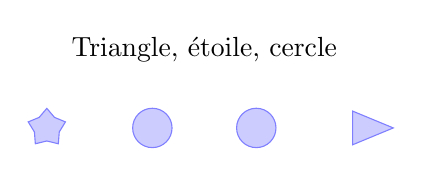
\begin{tikzpicture}
              \node at ( -0.66,0)  [circle,draw=blue!50,fill=blue!20,minimum size=5mm] {};
              \node at ( 0.66,0)  [circle,draw=blue!50,fill=blue!20,minimum size=5mm] {};
              \node at ( -2,0) [star,draw=blue!50,fill=blue!20] {};
              \node at ( 2,0)  [isosceles triangle,draw=blue!50,fill=blue!20] {};
              \node at (0,1.0) [black] {Triangle, étoile, cercle};
            \end{tikzpicture}
            \caption{Classification d'objet}
          \end{subfigure}
          \begin{subfigure}{0.4\textwidth}
            \centering
            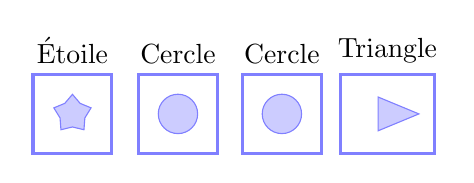
\begin{tikzpicture}
                % Draw the circle
                \node[circle, draw=blue!50, fill=blue!20, minimum size=5mm] (circle) at (-0.66,0) {};
                \node[draw=blue!50, very thick, minimum width=10mm, minimum height=10mm, anchor=center,label={Cercle}] at (circle) {};
                \node[circle, draw=blue!50, fill=blue!20, minimum size=5mm] (circle2) at (0.66,0) {};
                \node[draw=blue!50, very thick, minimum width=10mm, minimum height=10mm, anchor=center,label={Cercle}] at (circle2) {};
                \node [star,draw=blue!50,fill=blue!20] (star) at ( -2,0) {};
                \node[draw=blue!50, very thick, minimum width=10mm, minimum height=10mm, anchor=center,label={Étoile}] at (star) {};
                \node at ( 2,0)  [isosceles triangle,draw=blue!50,fill=blue!20] (triangle) {};
                \node[draw=blue!50, very thick, minimum width=12mm, minimum height=10mm, anchor=center,label={Triangle}] at (triangle) {};
                %\node at (0,2) [black] {Triangle, étoile, carré};
            \end{tikzpicture}
            \caption{Détection d'objet}
          \end{subfigure}~
          
          \begin{subfigure}{0.4\textwidth}
            \centering
            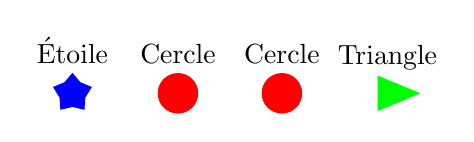
\begin{tikzpicture}
                %[background rectangle/.style={fill=black}, show background rectangle]
                % Draw the circle
                \node[circle, draw=red, fill=red, minimum size=5mm,label={Cercle}] (circle) at (-0.66,0) {};
                \node[circle, draw=red, fill=red, minimum size=5mm,label={Cercle}] (circle2) at (0.66,0) {};
                \node [star,draw=blue,fill=blue,label={Étoile}] (star) at ( -2,0) {};
                \node at ( 2,0)  [isosceles triangle,draw=green,fill=green,label={Triangle}] (triangle) {};
            \end{tikzpicture}
            \caption{Segmentation d'image}
          \end{subfigure}
          \begin{subfigure}{0.4\textwidth}
            \centering
            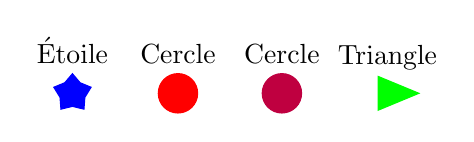
\begin{tikzpicture}
                %[background rectangle/.style={fill=black}, show background rectangle]
                % Draw the circle
                \node[circle, draw=red, fill=red, minimum size=5mm,label={Cercle}] (circle) at (-0.66,0) {};
                \node[circle, draw=purple, fill=purple, minimum size=5mm,label={Cercle}] (circle2) at (0.66,0) {};
                \node [star,draw=blue,fill=blue,label={Étoile}] (star) at ( -2,0) {};
                \node at ( 2,0)  [isosceles triangle,draw=green,fill=green,label={Triangle}] (triangle) {};
            \end{tikzpicture}
            \caption{Segmentation d'instance}
          \end{subfigure}
          \caption{Résultats de différentes méthodes de visiion par ordinateur pour une même image}
          \label{fig:computer_vision_problems}
      \end{figure}
  Les processus varient aussi dans leur résultante. Tandis que les modèles de segmentation pure feront une affectation de la même couleur à plusieurs objets d'un même type, la segmentation d'instance rend le processus de post-traitement des raster plus simple en donnant une couleur différente à chaque instance d'un même type d'objet. Cette dernière propriété a le mérite de potentiellement faciliter le post-traitement des résultats.
  \subsection{Algorithmes de segmentation sémantique basés sur la convolution}

  \subsubsection{U-Net}
    U-net a initialement été développé comme méthode de segmentation d'imagerie médicale par \textcite{ronneberger_u-net_2015}. Dans son implémentation initiale, le diagramme du réseau est donné à la figure \ref{fig:unet_arch}.
    \begin{figure}[!h]
      \centering
      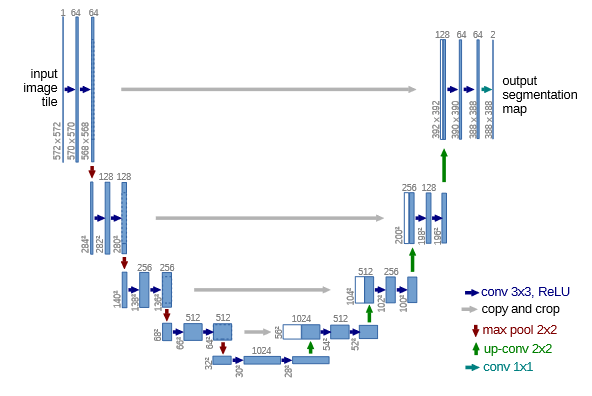
\includegraphics[width= 0.8 \textwidth]{unet_architecture.png}
      \caption{Architecture de réseau U-net \parencite{ronneberger_u-net_2015}}
      \label{fig:unet_arch}
    \end{figure}
    L'architecture peut être séparée en deux grandes phases. À gauche, il y a une phase d'encodage qui est constituée de 4 sous-blocs. Chaque sous-bloc est constitué de deux opérations de convolution 3x3 et d'activation \ac{ReLu} suivi d'un sous-échantillonnage utilisant max-pool pour augmenter le niveau d'abstraction, créer une carte de caractéristiques de plus en plus grossière et abstraite. Au niveau d'abstraction le plus haut, une carte de caractéristiques de 32x32 est créée au goulot d'étranglement du réseau. La partie de droite constitue le décodeur. Dans cette phase, la carte des caractéristiques des niveaux d'abstraction supérieurs est suréchantillonnée, concaténée avec le résultat de convolution, puis passe par une opération de double convolution. Le processus est répété jusqu'à revenir à la résolution de départ pour générer le masque de segmentation de l'image avec une convolution 1x1 finale. Plusieurs implémentations ont été trouvées qui créaient des masques de la même taille que l'image d'origine en utilisant du garnissage de zéro 
  \subsubsection{Dense U-Net}

  \subsubsection{DenseLabV3+}
  \subsection{Algorithmes de segmentation d'instance basés sur la convolution}
  La première est la segmentation sémantique qui consiste à séparer des pixels dans une image par classe. La deuxième est la segmentation d'instance. Cette dernière reconnait des objets, le classifie et en extrait le contour. \textcite{he_mask_2018} est l'article original sur la méthode qui a par la suite été adaptée dans un contexte de reconnaissance SIG \parencite{pesek_mask_2018} ou pour la reconnaissance automatique de terrains sportifs pour réinjecter les polygones directement dans \ac{OSM} \parencite{remillard_jremillardimages--osm_2024}.\par
  \textcite{fritz_instance_2020} développe plusieurs estimés de segmentation d'instance pour des bâtiments à l'aide de deux modèles. Le premier est celui cité plus haut\parencite{he_mask_2018} tandis que le deuxième est un modèle de segmentation d'image modifié pour segmenter les instances \parencite{iglovikov_ternausnetv2_2018} une fois la segmentation d'image complétée
  \subsection{Algorithmes de segmentation sémantique basée sur les transformeurs}
  \subsection{Algorithmes de segmentation d'instance basés sur les transformeurs}
  \subsection{Jeux de données disponibles à l'entrainement}
    Deux enjeux sont critiques au succès d'un projet d'apprentissage machine. La présence d'un modèle adapté à la tâche en cours et la présence d'un jeu de données annoté qui peut être utilisé pour ajuster les poids initiaux du modèle pour permettre de modifier les poids du modèle et permettre de l'appliquer à de grands ensembles de données. Le tableau suivant résumera les jeux de données actuellement disponibles pour la segmentation sémantique en milieu urbain:
    \begin{table}
      \centering
         \begin{tabular}{l p{0.2\textwidth} l p{0.3\textwidth}  p{0.2\textwidth} l} 
          \hline
          Nom & Origine & $N_{classes}$ & Classes pertinentes au stationnement & Point de vue\\
          \hline
          CNRParkEXT & \cite{amato_deep_2017} & 2 & Places occupées, places libres & Caméra de surveillance \\
          PKLot & \cite{de_almeida_pklot_2015} & 2 & Places occupées, places libres & Caméra de surveillance \\
          APKLot & \cite{hurst-tarrab_robust_2020} & 1 & Grappes & Imagerie satellite\\
          Skyscapes & \cite{azimi_skyscapes_2019} & 31 & Aires pavées, aires non-pavées & Orthophotos\\
          Grab-PkLot & \cite{yin_context-enriched_2022} & 1 & Aires de stationnement & Orthophotos\\
          \hline
        \end{tabular}
        \caption{Jeux de données annotés de segmentation sémantique en milieu urbain}
        \label{tab:jeux_donnees_segmentation_urbain}
    \end{table}
    \FloatBarrier
\Chapter{MÉTHODOLOGIE}\label{sec:Methodologie}
\section{Portée du chapitre}
Cette section portera sur la solution proposée pour répondre aux objectifs mis de l'avant en \ref{sec:obj_recherche}. Les sections \ref{sec:geopolitique_quebec} et \ref{sec:politiques_stationnement} donneront un aperçu de la géopolitique de la ville de Québec depuis la Deuxième Guerre mondiale et les modalités des codes d'urbanisme dans l'actuelle ville de Québec depuis 1995. La section \ref{sec:meth_donnees_dispo} présente les données disponibles pour évaluer l'inventaire de stationnement. La section \ref{sec:meth_urb_based_inventory} présente la méthodologie utilisée pour calculer l'inventaire basé sur les codes d'urbanisme de la ville de Québec, tandis que la section \ref{sec:meth_orthophoto} propose une méthodologie pour inférer la capacité basée sur les orthophotos. Finalement, les sections \ref{sec:meth_API,sec:meth_interface_web,sec:meth_analyse} montrent les détails de l'interface web, l'API et les méthodes d'analyse proposées.
\section{Géopolitique de la ville de Québec}\label{sec:geopolitique_quebec}
Cette section va faire un historique rapide de la géopolitique de la ville de Québec. Ceci est principalement pour dégager des grandes époques où les frontières sont restées stables et illustrer la complexité de représenter les règlements de plusieurs juridictions. \par
On observe trois grandes raflées de fusions \parencite{VilledeQuebec:ReperesChronologique:}:
\begin{itemize}
  \item '65-'72:
  \SubItem{Duberger('70), Les Saules('70) et Neufchâtel ('71) rejoignent la ville de Québec}
  \SubItem{Ste-Foy et Ancienne Lorette fusionnent('70)}
  \SubItem{Le territoire de Wendake s'étend vers le Sud}
  \SubItem{Orsainville cède une péninsule de territoire à Charlesbourg}
  \SubItem{Beauport et Beauport-Ouest fusionnent('66)}
  \SubItem{Notre-Dame de Lorette devient L'Ancienne-Lorette('67)}
  \item '72-76:
  \SubItem{Charlesbourg, Orsainville, Charlesbourg-Est et Notre-Dame des Laurentides fusionnent pour devenir Charlesbourg ('76)}
  \SubItem{Charlesbourg-Ouest est annexé par Québec('76)}
  \SubItem{Giffard, Beauport, Courville, Villeneuve et Montmorency fusionnent('76) pour devenir Beauport}
  \SubItem{Val-Belair et Val-Saint-Michel fusionnent et deviennent Val-Belair('73)}
  \item '76-2001:
  \SubItem{Stabilité des limites territoriales}
  \item 2002:
  \SubItem{Fusion de Québec, L'Ancienne-Lorette, St-Augustin de Desmaures, Charlesbourg, Beauport, Val-Belair, Ste-Foy, St-Émile, Lac-St-Charles, Vanier, Cap-Rouge et Loretteville}
  \item 2006
    \SubItem{Séparation St-Augustin de Desmaures et L'Ancienne-Lorette}
\end{itemize}
\FloatBarrier
La figure \ref{fig:municipalites_carto_historique} montre l'évolution des barrières géopolitiques au cours du temps. 
\begin{figure}[ht]
  \centering
  \begin{subfigure}[t]{0.45\textwidth}
    \centering
    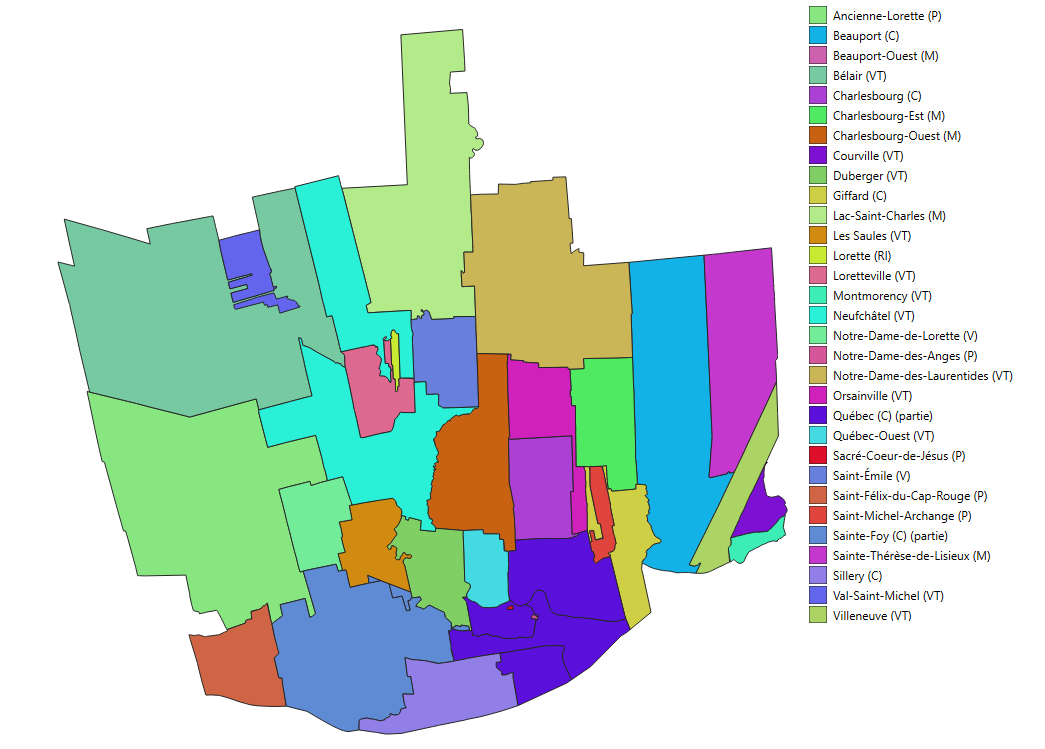
\includegraphics[width=0.9\linewidth]{images/municipalites_1965.png}
    \caption{1965}
    \label{fig:municipalites_1965}
  \end{subfigure}%
  \begin{subfigure}[t]{0.45\textwidth}
    \centering
    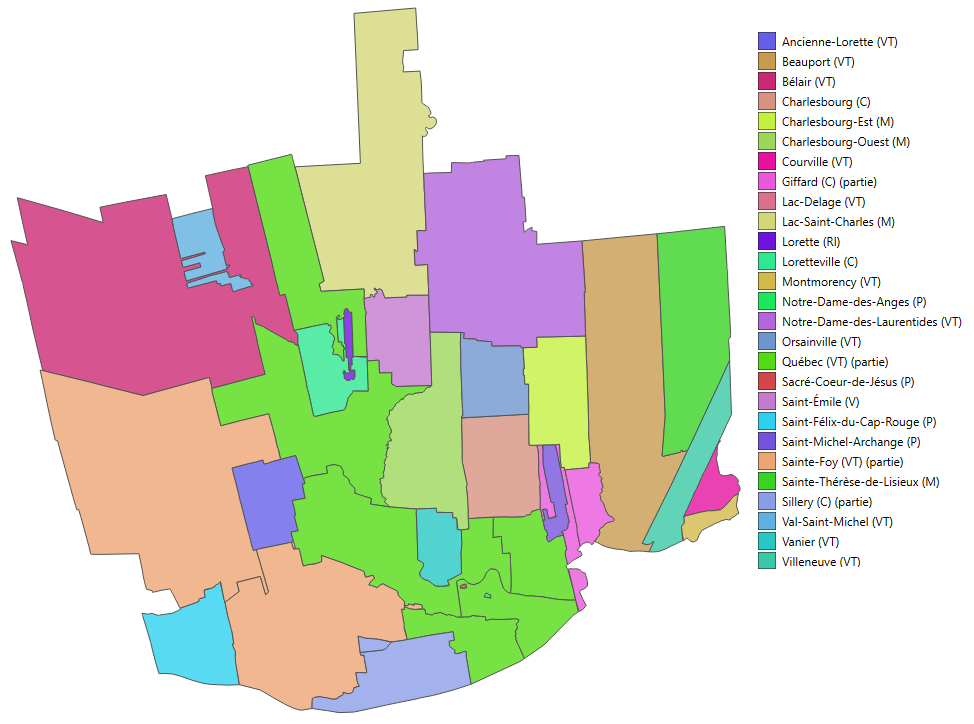
\includegraphics[width=0.9\linewidth]{images/municipalites_1972.png}
    \caption{1972}
    \label{fig:municipalites_1972}
  \end{subfigure}\\
  \begin{subfigure}[t]{0.45\textwidth}
    \centering
    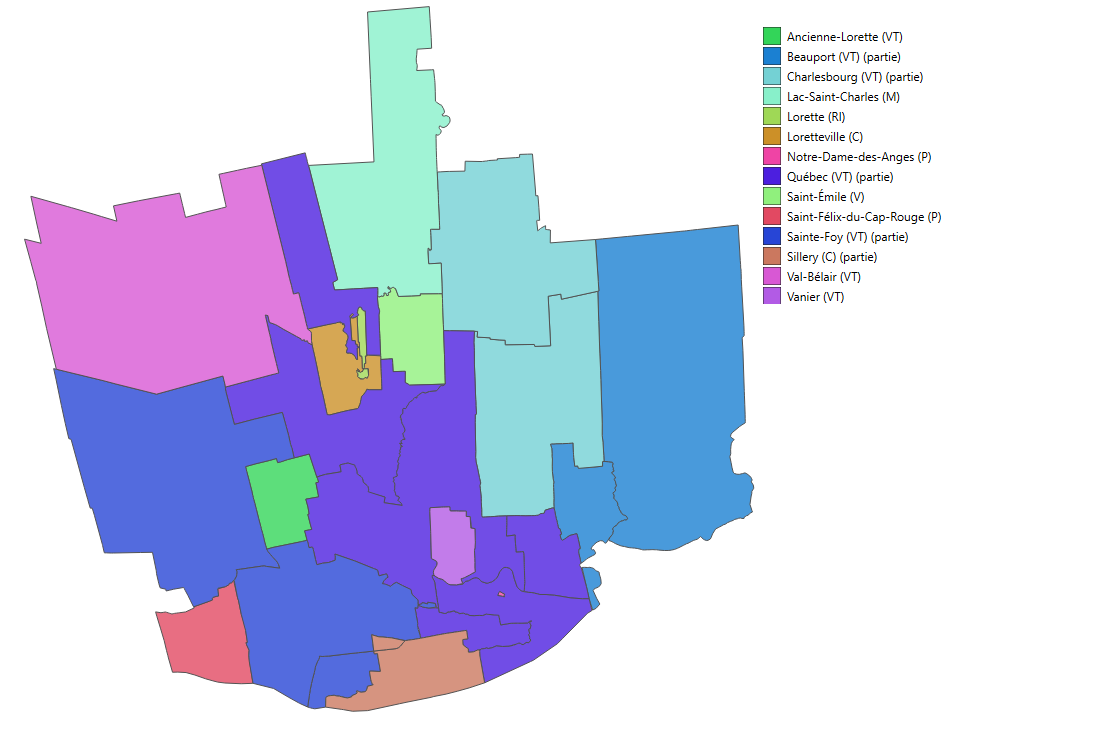
\includegraphics[width=0.9\linewidth]{images/municipalites_1980.png}
    \caption{1980}
    \label{fig:municipalites_1980}
  \end{subfigure}%
  \begin{subfigure}[t]{0.45\textwidth}
    \centering
    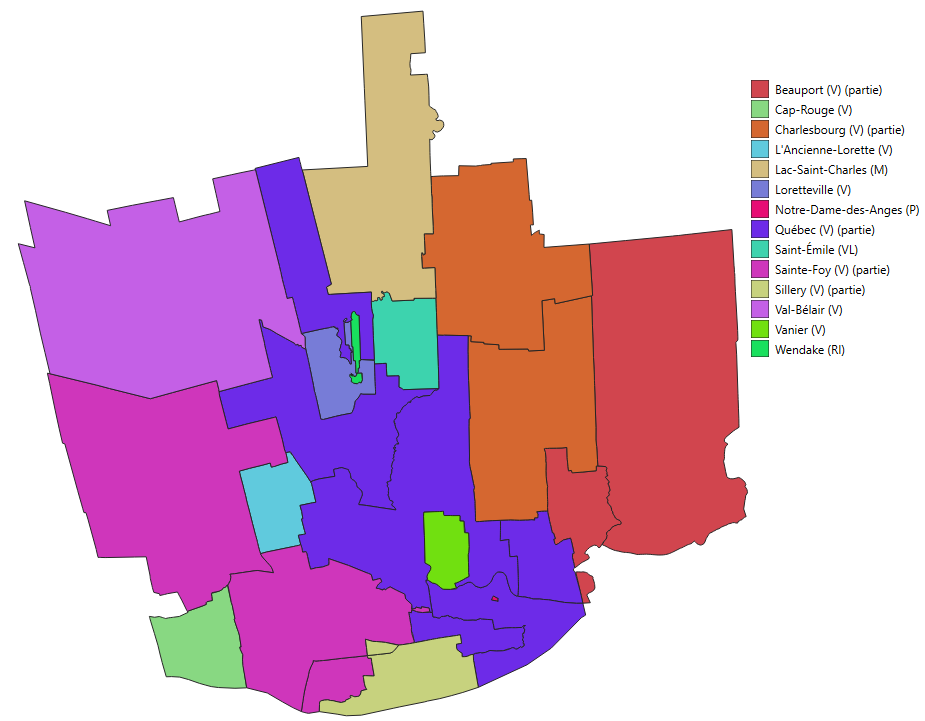
\includegraphics[width=0.9\linewidth]{images/municipalites_1988.png}
    \caption{1988}
    \label{fig:municipalites_1988}
  \end{subfigure}\\
  \begin{subfigure}[t]{0.45\textwidth}
    \centering
    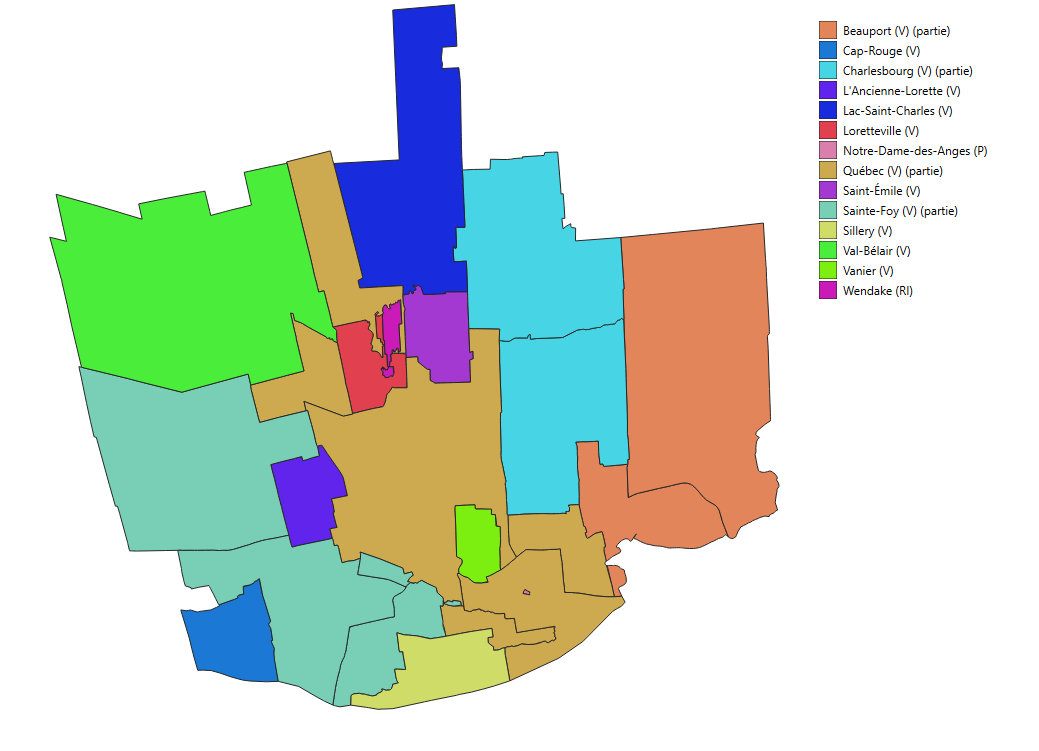
\includegraphics[width=0.9\linewidth]{images/municipalites_2001.png}
    \caption{2001}
    \label{fig:municipalites_2001}
  \end{subfigure}%
  \begin{subfigure}[t]{0.45\textwidth}
    \centering
    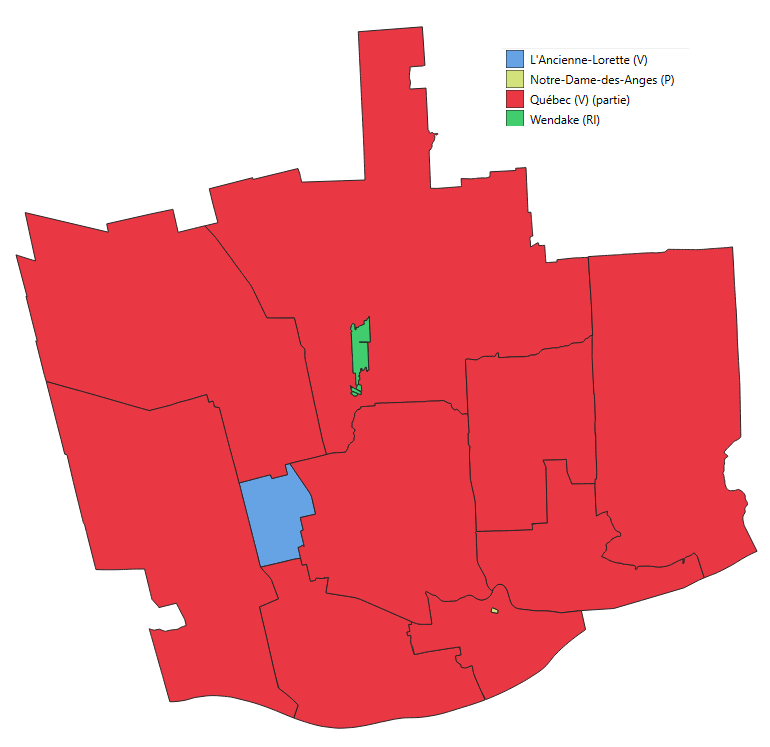
\includegraphics[width=0.8 \linewidth]{images/municipalites_2011.png}
    \caption{2011}
    \label{fig:municipalites_2011}
  \end{subfigure}%
  \caption{Séparation géopolitique du territoire de l'actuelle Ville de Québec \parencite{ElectionsQuebec:AtlasHistorique:2021}}\label{fig:municipalites_carto_historique}
\end{figure}

%Cela étant dit, l'historique de fusion de municipalités et la difficulté de trouver des codes d'urbanisme avant 1995 rend l'utilisation de ces données relativement difficile. La figure \ref{fig:historique_fusions} montre les fusions successives ayant mené à l'actuelle ville de Québec:
  %\begin{figure}[!h]
  %  \centering
  %  \captionsetup{justification=centering,margin=2cm}
  %  \includegraphics[width = 0.5\textwidth]{images/historique_fusions_VDQ.png}
  %  \captionsetup{justification=centering,margin=2cm}
  %  \caption{Diagramme montrant les fusions géopolitiques de la ville de Québec. \hl{Vérifier droits d'auteurs} Source: }
  %  \label{fig:historique_fusions}
  %\end{figure}
  %\FloatBarrier

%D'autre part, à travers les années '90, la ville de Québec va créer des requis de statinnement différents par quartiers. Post-fusion, les différentes villes garderont leurs codes d'urbanisme jusqu'en 2009 où la ville créera un code applicable à l'ensemble du territoire avec 4 sous zone: Général, Axe Structurant B, Axe Structurant A et Urbain Dense \parencite{VilledeQuebec:ReglementHarmonisation:2009}. La définition spatiale des unités de voisinage est donnée dans \textcite{VilledeQuebec:ZonageMunicipal:2024} et l'assignation de la zone est donnée dans \textcite{VilledeQuebec:GrilleSpecifications:2024}. La carte à la figure \ref{fig:types_unites_voisinage} montre les unités de voisinage pour la ville de Québec catégorisé selon la définition ci-haut:
\begin{figure}[ht]
  \centering
  \begin{subfigure}[t]{0.5\textwidth}
    \centering
    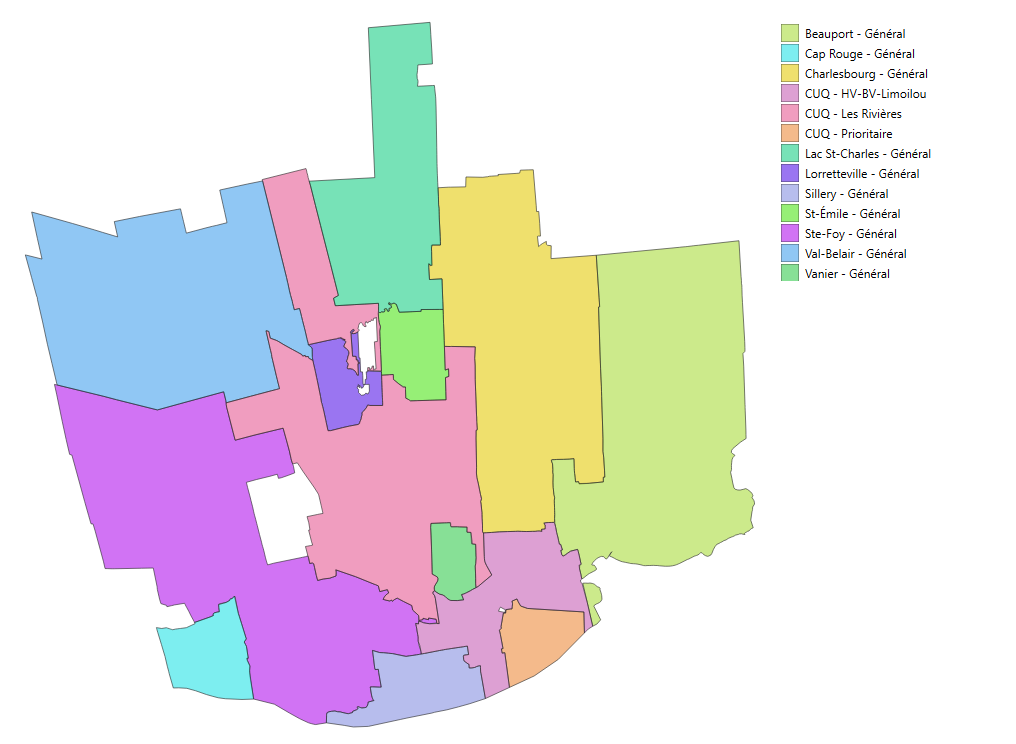
\includegraphics[width=0.9\linewidth]{images/geographie_code_urbanisme_1995-1997.png}
    \caption{1995-1997}
  \end{subfigure}~
  \begin{subfigure}[t]{0.5\textwidth}
    \centering
    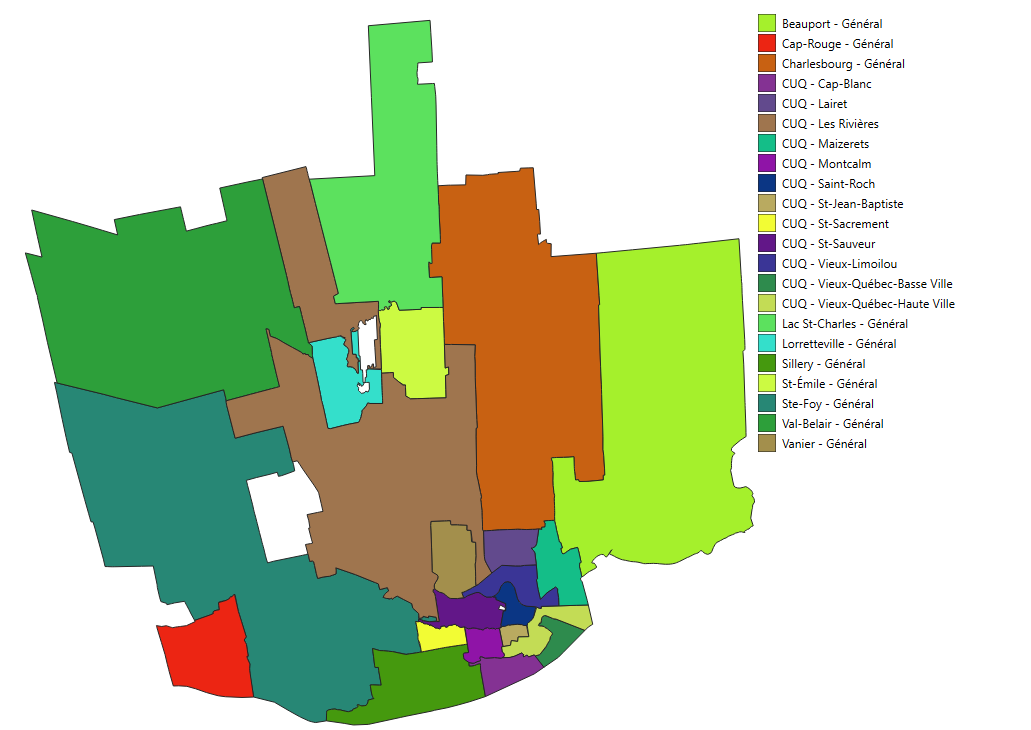
\includegraphics[width=0.9\linewidth]{images/geographie_code_urbanisme_1997-2009.png}
    \caption{1995-1997}
  \end{subfigure}\\
  \begin{subfigure}[t]{0.6\textwidth}
  \centering
  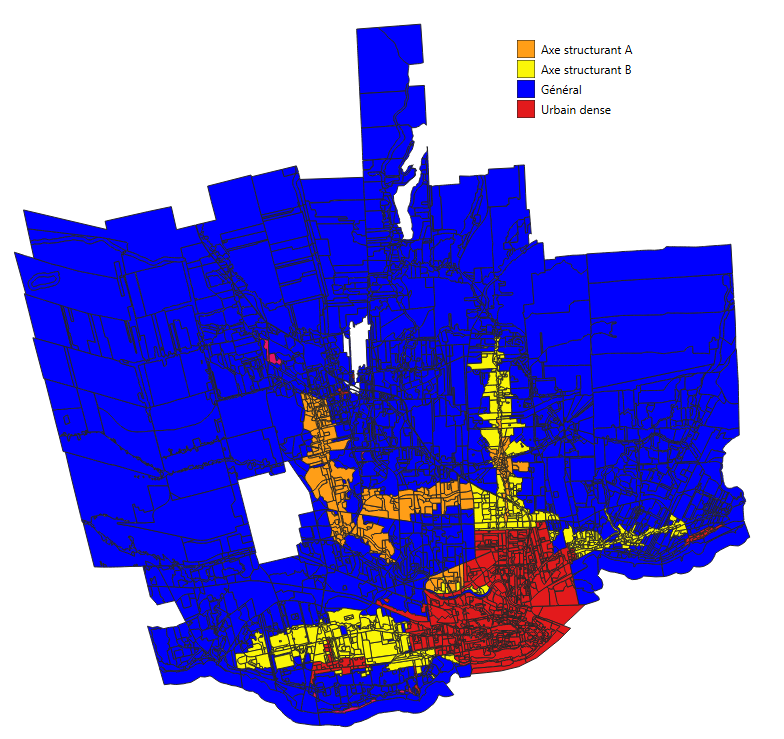
\includegraphics[width=0.8\linewidth]{images/geographie_code_urbanisme_2009_present.png}
  \caption{2010-présent}
  \end{subfigure}
  \caption{Secteur ayant des minimum de stationnement différents}
  \label{fig:types_unites_voisinage}
\end{figure}
\FloatBarrier
\section{Politiques de stationnement de la ville de Québec} \label{sec:politiques_stationnement}

La ville de Québec est en processus d'abroger ces requis pour l'habitation pour les zones en milieu dense ou le long des axes de transport en commun \parencite{VilledeQuebec:AdoptionReglement:2024}.\par
  En plus de l'hétérogénéité spatiale qui est décrite à la section \ref{sec:geopolitique_quebec}, on constate aussi une hétérogénéité au niveau des catégories utilisées pour les requis de stationnement. Ceci est d'autant plus ardu que les catégories utilisées dans les minimums de stationnement n'ont pas nécessairement d'équivalent direct dans le \ac{CUBF} utilisé dans le rôle foncier du Québec \parencite[Annexe 2C.1]{GouvernementduQuebec:ManuelEvaluation:2024}. Le tableau \ref{tab:req_stat_presents} et la figure \ref{fig:n_utilisation_CUBF_minimums} résument la présence d'un requis de stationnement explicité ou inféré pour un code \ac{CUBF} donné \parencite{VilledeQuebec:AdoptionReglement:2024,VilledeQuebec:ReglementZonage:1995}. Les codes d'urbanisme des municipalités pré-fusion sont issus d'un résumé fourni par la ville. Cette synthèse est nécessairement arbitraire: les catégories dans le code d'urbanisme ne sont pas constantes entre les codes avec différents niveaux de superposition ou catégorisation par municipalité, rendant une synthèse difficile. La synthèse est recalée sur les codes \ac{CUBF} pour la simple raison que cette donnée sera exploitée pour choisir la réglementation à appliquer pour inférer une capacité de stationnement requise. Les données sont issues d'une synthèse de la ville. Une demande a été complétée auprès du service de greffe pour obtenir les textes de loi.
  %\tiny
  \newcommand{\YCHECK}{\Checkmark}
  \newcommand{\NCHECK}{\cellcolor{red} \XSolid}
  \newcommand{\OCHECK}[1]{\cellcolor{orange} / #1}
  \newcolumntype{P}[1]{>{\centering\arraybackslash}p{#1}}
  \newcolumntype{M}[1]{>{\centering\arraybackslash}m{#1}}
  
  \setlength{\LTcapwidth}{\textwidth}
  \begin{landscape}
    \begin{center}
      \begin{longtable}{P{1.0cm} | p{7.5cm} | c || *{12}{P{5mm}}||p{6mm}} 
        \multirow{2}{*}{\STAB{\rotatebox[origin=c]{90}{Categ}}} & Juridiction & \STAB{\rotatebox[origin=c]{90}{Code \ac {CUBF}}} & \rotatebox[origin=c]{90}{  VDQ (2009-présent)} & \rotatebox[origin=c]{90}{VDQ (1995-2009)} & \rotatebox[origin=c]{90}{Beauport} & \rotatebox[origin=c]{90}{Cap-Rouge} & \rotatebox[origin=c]{90}{Charlesbourg} & \rotatebox[origin=c]{90}{Lac St-Charles} & \rotatebox[origin=c]{90}{Loretteville} & \rotatebox[origin=c]{90}{Sillery} & \rotatebox[origin=c]{90}{Ste-Foy} & \rotatebox[origin=c]{90}{St-Émile} & \rotatebox[origin=c]{90}{Val-Belair} & \rotatebox[origin=c]{90}{Vanier} & \rotatebox[origin=c]{90}{Nombre de requis} \\
        %& No. Règl. & MEFQ & R.V.Q. 1400 & V.Q.Z. 3 & 87-806 & 1151-95 & 96-2921 & 88-257 & 1386 & 950 & 3501 & 310-89 & VB-344-88 & 93-05-1245\\
        \hline  
        \endhead
        \hline
        \multicolumn{15}{c}{\Checkmark = Requis présent, \colorbox{red}{\XSolid} = Requis absent, \colorbox{orange}{/} = Requis implicite à une définition plus générale}\\\hline
        \endfoot
        \hline
        \multicolumn{15}{c}{\Checkmark = Requis présent, \colorbox{red}{\XSolid} = Requis absent, \colorbox{orange}{/} = Requis implicite à une définition plus générale}\\\hline
        \caption{Présence de règlementation de stationnement selon le code \ac{CUBF}}\label{tab:req_stat_presents}
        \endlastfoot
        \multirow{6}{*}{\STAB{\rotatebox[origin=c]{90}{Résidentiel}}} & Logement & 10XX & \YCHECK & \YCHECK &\YCHECK & \YCHECK &\YCHECK &\YCHECK& \YCHECK & \YCHECK & \YCHECK &\YCHECK & \YCHECK & \YCHECK&12\\
        & Logement subventionné & 10XX & \YCHECK & \YCHECK & \NCHECK & \NCHECK & \NCHECK& \NCHECK &\NCHECK &\NCHECK &\NCHECK &\NCHECK &\NCHECK & \NCHECK&2 \\
        & Habitation Collectives & 15XX & \YCHECK & \NCHECK & \YCHECK & \YCHECK & \YCHECK & \YCHECK & \YCHECK & \NCHECK & \NCHECK & \YCHECK & \YCHECK & \NCHECK&8 \\
        & Maison de chambres &  151X & \YCHECK & \YCHECK & \OCHECK{} & \OCHECK{} & \OCHECK{} & \OCHECK{} & \YCHECK & \NCHECK & \YCHECK &\OCHECK{} & \YCHECK & \YCHECK&6\\
        & Maison de retraite non autonomes & 1541 & \OCHECK{} & \YCHECK & \YCHECK & \YCHECK & \OCHECK{} & \OCHECK{} & \YCHECK & \YCHECK & \YCHECK & \OCHECK{} & \OCHECK{} & \NCHECK &6\\
        & Maison de retraite autonomes & 1543 & \OCHECK{} & \YCHECK & \YCHECK & \YCHECK & \OCHECK{} & \OCHECK{} & \YCHECK & \YCHECK & \YCHECK & \OCHECK{} & \OCHECK{} & \NCHECK&6 \\ 
        \hline
        \multirow{7}{*}{\STAB{\rotatebox[origin=c]{90}{Industriel / Infra.}}}& Industriel Général & \makecell[l]{2XXX\\3XXX} & \YCHECK & \YCHECK & \YCHECK & \YCHECK & \YCHECK & \YCHECK & \YCHECK & \YCHECK & \YCHECK & \YCHECK & \YCHECK & \YCHECK&12 \\
        & Industrie Haute Technologie & \makecell[l]{355X\\356X\\357X} & \YCHECK & \OCHECK{} & \OCHECK{}  & \OCHECK{}  & \OCHECK{}   & \OCHECK{}   & \OCHECK{}   & \OCHECK{}   &  \YCHECK & \OCHECK{}   & \OCHECK{}& \OCHECK{}&2 \\
        & Industrie mise en valeur et récupération &487X & \YCHECK & \OCHECK{} & \OCHECK{} & \OCHECK{} & \OCHECK{} & \OCHECK{} & \OCHECK{} & \OCHECK{} & \YCHECK & \OCHECK{} & \OCHECK{} & \OCHECK{}&2 \\ 
        & Entreposage & 637X & \YCHECK&\YCHECK&\OCHECK{}&\OCHECK{}&\OCHECK{}&\OCHECK{}&\YCHECK&\YCHECK&\OCHECK{}&\YCHECK&\YCHECK&\YCHECK &7\\
        & Service de construction & 66XX & \OCHECK{}  & \OCHECK{} &\OCHECK{} &\OCHECK{} &\OCHECK{} &\OCHECK{} & \YCHECK &\OCHECK{} &\OCHECK{} & \OCHECK{} & \OCHECK{} & \YCHECK&2\\
        \hline
        \multirow{4}{*}{\STAB{\rotatebox[origin=c]{90}{Commerces}}} & Centre et Immeuble Commercial & 50XX & \YCHECK & \YCHECK & \YCHECK & \YCHECK &\YCHECK&\YCHECK& \YCHECK&\YCHECK&\YCHECK&\YCHECK&\YCHECK&\YCHECK&12\\
        & Vente en gros & 51XX &\OCHECK{}&\YCHECK&\OCHECK{}&\OCHECK{}&\OCHECK{}&\OCHECK{}&\YCHECK&\OCHECK{}&\OCHECK{}&\OCHECK{}&\YCHECK&\OCHECK{}&3\\
        & Vente au détail construction et quincaillerie & 52XX&\OCHECK{}&\OCHECK{}&\OCHECK{}&\YCHECK&\OCHECK{}&\OCHECK{}&\YCHECK&\YCHECK&\YCHECK&\OCHECK{}&\YCHECK&\OCHECK{}&5 \\
        & Vente au détail marchandises & 53XX&\OCHECK{}&\OCHECK{}&\OCHECK{}&\OCHECK{}&\OCHECK{}&\OCHECK{}&\OCHECK{}&\OCHECK{}&\OCHECK{}&\OCHECK{}&\OCHECK{}&\OCHECK{}&0\\
        \multirow{6}{*}{\STAB{\rotatebox[origin=c]{90}{Commerces}}} & Vente au détail de l'alimentation & 54XX &\YCHECK&\YCHECK&\OCHECK{}&\OCHECK{}&\YCHECK&\YCHECK&\YCHECK&\YCHECK&\YCHECK&\YCHECK&\YCHECK&\YCHECK &10\\
        & Vente au détail de véhicules et produits connexes & 55XX &\YCHECK&\OCHECK{}&\OCHECK{}&\OCHECK{}&\OCHECK{}&\YCHECK&\YCHECK&\YCHECK&\YCHECK&\YCHECK&\YCHECK&\YCHECK&8\\
        & Station Essence & 553X&\YCHECK&\YCHECK&\YCHECK&\OCHECK{}&\OCHECK{}&\OCHECK{}&\YCHECK&\OCHECK{}&\YCHECK&\YCHECK&\YCHECK&\YCHECK&7 \\
        & Vente au détail de vêtements & 56XX&\OCHECK{}&\OCHECK{}&\OCHECK{}&\OCHECK{}&\OCHECK{}&\OCHECK{}&\YCHECK&\OCHECK{}&\YCHECK&\OCHECK{}&\OCHECK{}&\OCHECK{}&2\\
        & Vente au détail de mobilier & 57XX&\YCHECK&\YCHECK&\OCHECK{}&\OCHECK{}&\OCHECK{}&\OCHECK{}&\YCHECK&\OCHECK{}&\OCHECK{}&\OCHECK{}&\OCHECK{}&\OCHECK{}&3 \\
        & Vente au détail Autre & 59XX&\OCHECK{}&\OCHECK{}&\OCHECK{}&\OCHECK{}&\OCHECK{}&\OCHECK{}&\OCHECK{}&\OCHECK{}&\OCHECK{}&\OCHECK{}&\OCHECK{}&\OCHECK{}&0\\
        \hline
        \multirow{7}{*}{\STAB{\rotatebox[origin=c]{90}{Restaurants et bars}}} & Restaurant & 581X & \YCHECK&\NCHECK&\YCHECK&\NCHECK&\YCHECK&\YCHECK&\YCHECK&\YCHECK&\YCHECK &\YCHECK&\YCHECK&\YCHECK&7 \\
        & Restaurant plein service & \makecell{5811 \\ 5812 \\ 5815}& \OCHECK{}&\YCHECK&\OCHECK{}&\YCHECK&\OCHECK{}&\OCHECK{}&\OCHECK{}&\OCHECK{}&\OCHECK{}&\OCHECK{}&\OCHECK{}&\OCHECK{}&2\\
        & Restaurant service restreint/libre service& \makecell{5811 \\ 5812 }& \OCHECK{}&\YCHECK&\OCHECK{}&\YCHECK&\OCHECK{}&\OCHECK{}&\OCHECK{}&\OCHECK{}&\OCHECK{}&\OCHECK{}&\OCHECK{}&\OCHECK{}&2\\
        & Débit d'alcool & 582X&\YCHECK&\YCHECK&\YCHECK&\YCHECK&\YCHECK&\YCHECK&\YCHECK&\YCHECK&\YCHECK&\YCHECK&\YCHECK&\YCHECK&11\\
        \hline
        \multirow{3}{*}{\STAB{\rotatebox[origin=c]{90}{Tourisme}}} & Établissement d'hébergement & 583X&\YCHECK&\NCHECK&\NCHECK&\YCHECK&\YCHECK&\YCHECK&\YCHECK&\YCHECK&\YCHECK&\YCHECK&\YCHECK&\YCHECK&10\\
        & Hôtel & 5831&\OCHECK{}&\YCHECK&\YCHECK&\OCHECK{}&\OCHECK{}&\OCHECK{}&\OCHECK{}&\OCHECK{}&\OCHECK{}&\OCHECK{}&\OCHECK{}&\OCHECK{}&2\\
        & Môtel & 5832&\OCHECK{}&\YCHECK&\YCHECK&\OCHECK{}&\OCHECK{}&\OCHECK{}&\OCHECK{}&\OCHECK{}&\OCHECK{}&\OCHECK{}&\OCHECK{}&\OCHECK{}&2\\
        \hline
        & Services & 6XXX & \YCHECK & \YCHECK & \YCHECK &\YCHECK & \YCHECK & \YCHECK & \YCHECK & \YCHECK &\YCHECK &\NCHECK &\YCHECK&\NCHECK&10\\
        & Immeubles à bureaux & 60XX&\YCHECK&\YCHECK&\OCHECK{}&\YCHECK&\YCHECK&\YCHECK&\YCHECK&\YCHECK&\YCHECK&\NCHECK&\YCHECK&\NCHECK&9\\
        \multirow{19}{*}{\STAB{\rotatebox[origin=c]{90}{Services}}}& Finance, Assurance et Service immobilier & 61XX&\OCHECK{}&\YCHECK&\OCHECK{}&\OCHECK{}&\OCHECK{}&\OCHECK{}&\YCHECK&\OCHECK{}&\OCHECK{}&\YCHECK&\OCHECK{}&\YCHECK&4\\
        & Banque & 611X&\OCHECK{}&\YCHECK&\OCHECK{}&\YCHECK&\OCHECK{}&\YCHECK&\YCHECK&\YCHECK&\YCHECK&\OCHECK{}&\YCHECK&\OCHECK{}&7\\
        & Service personnels & 62XX & \OCHECK{} &\OCHECK{}&\OCHECK{}&\OCHECK{}&\YCHECK&\OCHECK{}& \OCHECK{}&\OCHECK{}&\YCHECK&\OCHECK{} &\OCHECK{}&\OCHECK{}&2\\
        & Salon de beauté / coiffure& 623X& \OCHECK{}&\YCHECK&\OCHECK{}&\OCHECK{}&\OCHECK{}&\OCHECK{}&\YCHECK&\OCHECK{}&\OCHECK{}&\OCHECK{}&\OCHECK{}&\YCHECK &3\\
        & Salon funéraire& 624X&\YCHECK&\YCHECK&\YCHECK&\YCHECK&\YCHECK&\YCHECK&\YCHECK&\YCHECK&\YCHECK&\YCHECK&\YCHECK&\YCHECK&12\\
        & Services d'affaires & 63XX &\OCHECK{}&\OCHECK{}&\YCHECK&\OCHECK{}&\OCHECK{}&\OCHECK{}&\YCHECK&\OCHECK{}&\OCHECK{}&\YCHECK&\OCHECK{}&\YCHECK&4\\
        & Services de réparation & 64XX&\OCHECK{}&\OCHECK{}&\OCHECK{}&\OCHECK{}&\OCHECK{}&\OCHECK{}&\OCHECK{}&\OCHECK{}&\OCHECK{}&\OCHECK{}&\OCHECK{}&\OCHECK{}&0\\
        & Service de réparation d'automobiles&641X&\YCHECK&\YCHECK&\YCHECK&\YCHECK&\OCHECK{}&\OCHECK{}&\YCHECK&\OCHECK{}&\YCHECK&\YCHECK&\YCHECK&\YCHECK&9\\
        & Service de réparation de mobiliers, d'équipements et de machines & 642X&\OCHECK{}&\OCHECK{}&\OCHECK{}&\OCHECK{}&\OCHECK{}&\OCHECK{}&\YCHECK&\OCHECK{}&\OCHECK{}&\OCHECK{}&\OCHECK{}&\OCHECK{}&1\\ 
        & Service de réparation de véhicules légers& 643X&\YCHECK&\YCHECK&\YCHECK&\YCHECK&\OCHECK{}&\OCHECK{}&\YCHECK&\OCHECK{}&\YCHECK&\YCHECK&\YCHECK&\YCHECK&9\\
        & Service de réparation et d'entretien de véhicules lourds& 644X&\YCHECK&\YCHECK&\YCHECK&\YCHECK&\OCHECK{}&\OCHECK{}&\YCHECK&\OCHECK{}&\YCHECK&\YCHECK&\YCHECK&\YCHECK&9\\
        & Service professionnel & 65XX&\YCHECK&\OCHECK{}&\YCHECK&\YCHECK&\OCHECK{}&\OCHECK{}&\OCHECK{}&\OCHECK{}&\OCHECK{}&\OCHECK{}&\OCHECK{}&\OCHECK{}&0\\
        & Service médical et de santé & 651X&\YCHECK&\YCHECK&\OCHECK{}&\OCHECK{}&\YCHECK&\YCHECK&\YCHECK&\YCHECK &\YCHECK & \OCHECK{} &\YCHECK & \OCHECK{}&9\\
        & Service d'hôpital & 6513 &\YCHECK &\YCHECK &\YCHECK &\YCHECK&\YCHECK&\YCHECK&\YCHECK&\YCHECK&\YCHECK&\YCHECK&\YCHECK&\YCHECK&12\\
        & Sanatorium, maison de convalescence et de repos & 6516 &\YCHECK &\YCHECK &\YCHECK&\OCHECK{}&\YCHECK &\YCHECK&\YCHECK&\YCHECK&\YCHECK&\YCHECK&\YCHECK&\YCHECK&11\\
        \multirow{12}{*}{\STAB{\rotatebox[origin=c]{90}{Services}}}& Service gouvernemental&67XX&\OCHECK{} & \OCHECK{} &\OCHECK{}&\OCHECK{}&\OCHECK{} &\OCHECK{} & \YCHECK&\OCHECK{}&\YCHECK&\YCHECK&\YCHECK&\YCHECK &5 \\
        & Pompiers/Police &672X&\YCHECK & \YCHECK &\OCHECK{}&\OCHECK{} &\OCHECK{} & \OCHECK{}&\OCHECK{}&\YCHECK&\OCHECK{}&\YCHECK&\OCHECK{}&\OCHECK{}&4\\
        & Service éducationnel&68XX&\YCHECK&\YCHECK&\NCHECK&\YCHECK&\NCHECK&\YCHECK&\YCHECK&\YCHECK&\NCHECK&\YCHECK{}&\YCHECK&\YCHECK &9 \\
        & Service de garderie&6541&\YCHECK&\OCHECK{}&\OCHECK{}&\OCHECK{}& \YCHECK&\OCHECK{}& \YCHECK &\OCHECK{}&\YCHECK&\OCHECK{}&\YCHECK&\OCHECK{}&5 \\
        & École Maternelle&6811&\OCHECK{}&\OCHECK{}&\OCHECK{}&\OCHECK{}&\OCHECK{}&\OCHECK{}&\YCHECK&\OCHECK{}&\YCHECK&\OCHECK{}&\YCHECK{}&\YCHECK{}&4 \\
        & École Primaire&6812&\YCHECK&\YCHECK&\YCHECK&\YCHECK&\YCHECK&\YCHECK&\YCHECK&\YCHECK&\YCHECK&\OCHECK{}&\YCHECK&\YCHECK&11 \\
        & École Secondaire / Polyvalente&\makecell{6813\\6822}&\YCHECK&\YCHECK&\YCHECK&\OCHECK{}&\YCHECK& \YCHECK&\YCHECK&\YCHECK&\YCHECK&\OCHECK{}&\YCHECK&\YCHECK&10 \\
        & CÉGEP &6823&\YCHECK&\YCHECK&\YCHECK&\OCHECK{}&\OCHECK{}&\YCHECK&\YCHECK&\OCHECK{}&\YCHECK&\OCHECK{}&\OCHECK{}&\OCHECK{}&6\\
        & Université&6821&\YCHECK&\YCHECK&\YCHECK&\OCHECK{}&\YCHECK&\YCHECK&\YCHECK&\OCHECK{}&\YCHECK&\OCHECK{}&\OCHECK{}&\OCHECK{}&7\\ 
        & Services religieux &691X&\YCHECK&\OCHECK{}&\YCHECK&\YCHECK&\OCHECK{}&\YCHECK&\YCHECK&\YCHECK&\YCHECK&\OCHECK{}&\YCHECK&\YCHECK&9\\
        \hline
        \multirow{8}{*}{\STAB{\rotatebox[origin=c]{90}{Culture et Récréation}}} & Culture, Récréation et Loisirs&7XXX &\NCHECK&\YCHECK&\YCHECK&\NCHECK&\YCHECK&\YCHECK&\NCHECK&\YCHECK&\NCHECK&\YCHECK&\YCHECK&\YCHECK&8\\
        & Activité Culturelle(Musée, Biblio) &711X&\YCHECK&\YCHECK&\YCHECK&\YCHECK&\YCHECK&\YCHECK&\YCHECK&\YCHECK&\YCHECK &\OCHECK{} &\OCHECK{} &\OCHECK{}&9\\
        & Assemblée de loisirs(Théâtre, Cinéma) &721X&\YCHECK&\YCHECK&\YCHECK& \YCHECK& \YCHECK&\YCHECK&\YCHECK&\YCHECK&\YCHECK&\OCHECK{}&\YCHECK&\OCHECK{}&10 \\
        & Installation sportive (Stade, Hippodrome)&722X&\YCHECK&\OCHECK{}&\OCHECK{}&\NCHECK&\OCHECK{}&\OCHECK{}&\YCHECK&\OCHECK{}&\YCHECK&\OCHECK{}&\OCHECK{}&\OCHECK{}&3\\
        & Centre de congrès&723X& \OCHECK{} & \YCHECK & \OCHECK{} & \NCHECK & \OCHECK{} & \OCHECK{}& \YCHECK& \OCHECK{} & \OCHECK{} & \OCHECK{} & \OCHECK{} & \OCHECK{}&2 \\
        & Activités récréatives&74XX&\YCHECK&\OCHECK{}&\YCHECK&\NCHECK&\OCHECK{}&\OCHECK{}&\YCHECK&\OCHECK{}&\YCHECK&\OCHECK{}&\OCHECK{}&\OCHECK{} &4\\
        & Terrains de golf&\makecell{7411\\7412}& \YCHECK& \OCHECK{}&\OCHECK{}&\NCHECK&\OCHECK{}&\OCHECK{}&\YCHECK&\OCHECK{}&\YCHECK&\YCHECK&\OCHECK{}&\OCHECK{}&4\\
        & Arena& 7451& \YCHECK&\YCHECK&\OCHECK{}&\NCHECK&\OCHECK{}&\OCHECK{}&\YCHECK{}&\YCHECK&\OCHECK{}&\YCHECK&\YCHECK&\OCHECK{}&6\\
        & Parcs/Camps &\makecell{75XX\\76XX}&\YCHECK &\NCHECK&\NCHECK&\NCHECK&\NCHECK&\NCHECK&\NCHECK&\NCHECK&\YCHECK&\YCHECK&\NCHECK&\YCHECK&5 \\
        \hline
        N/A & Extraction de ressources / Agriculture & 8XXX&\YCHECK&\NCHECK&\NCHECK&\NCHECK&\NCHECK&\NCHECK&\YCHECK&\NCHECK&\YCHECK&\NCHECK&\NCHECK&\NCHECK&3\\
      \end{longtable}
    \end{center}  
    \begin{figure}[h]
      \centering
      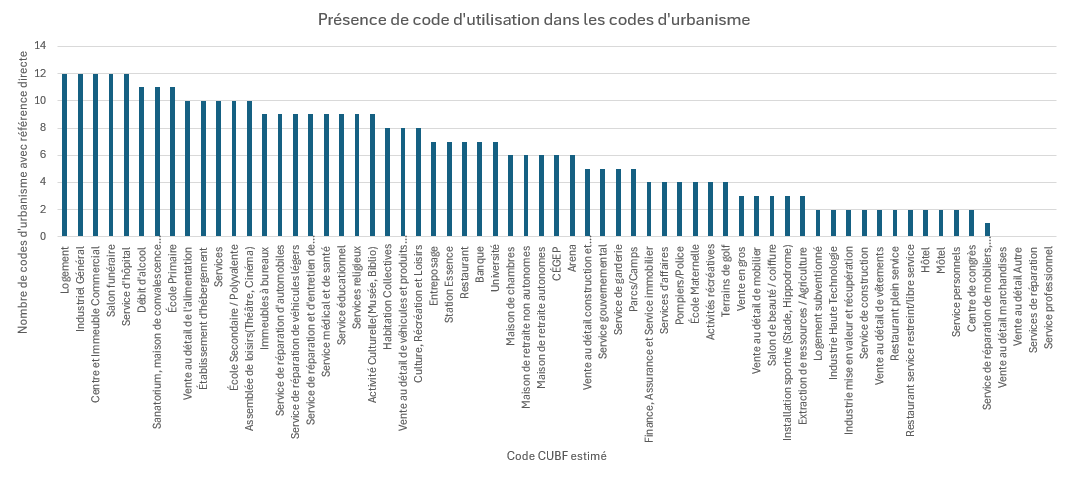
\includegraphics[width=22cm]{images/presence_requis_par_CUBF}
      \caption{Nombre de codes d'urbanisme utilisant les codes d'utilisation listés}\label{fig:n_utilisation_CUBF_minimums}
    \end{figure}
  \end{landscape}
  %\normalsize
  \FloatBarrier
  
  Les objets sur lesquels sont basés les codes d'urbanisme sont aussi hétérogènes. Bien que la plupart des requis soient basé sur une surface de plancher, certains sont exprimés en fonction d'autres objets considérés pertinents. D'autre part, la même utilisation du sol n'est pas nécessairement légiférée en utilisant le même objet entre deux juridictions différentes. Le tableau \ref{tab:objet_pour_inference_capacite} synthétise les objets considérés et les usages pour lesquels ils sont utilisés.

  \begin{table}[h]
    \centering
    \begin{tabular}{p{4cm} p{8cm}}
      \hline
      Objets considéré & Usages pertinents \\
      \hline
      Superficie de plancher & Majoritaire\\
      Superficie par usage (bureau, plateau TV) & Station télé \\
      Superficie de terrain & parc, zoo \\
      Logement & Logement \\
      Chambres & Maison de chambres, hébergement touristique, établissement de santé\\
      Lit & Établissement de santé, auberges de jeunesse, établissement carcéral \\
      Baie de service & Commerces liés à l'automobile\\
      Siège & Lieux de rassemblement, cinéma, théâtres, stades \\
      Salle & Cabinet médical, établissement scolaire, salon funéraire\\
      Personne & Débit d'alcool\\
      Employé & Services et vente au détail\\
      Médecin & Établissement de santé\\
      Étudiant & Établissement scolaire\\
      Plateau sportif & Golf, tennis, quilles, billards\\
      Poste de travail & Services personnels (salon de beauté)\\
      \hline
    \end{tabular}
    \caption{Récapitulatif des objets considérés pour fixer les capacité de stationnement}\label{tab:objet_pour_inference_capacite}
  \end{table}
  

  \FloatBarrier

\section{Données de départ}\label{sec:meth_donnees_dispo}
  \subsection{\ac{SIG}}
    \subsubsection{Synthèse des données disponibles}
      Le tableau \ref{tab:donnees_disponibles_Québec} résume les données disponibles pour la ville de Québec et leur source.
      \begin{landscape}
        \LTcapwidth=\textwidth
      \begin{longtable}[h!]{p{.2 \linewidth} p{.1 \linewidth} p{.3 \linewidth} p{.15\linewidth} p{.125\linewidth} }
        
        
        \hline
        Géobase & Type & Description  & Source & Date téléchargement.\\ 
        \hline
        \hline
        \endhead
        \hline
        \endfoot
        \hline
        \caption{Géobases pour le territoire de la ville de Québec}
        \label{tab:donnees_disponibles_Québec}
        \endlastfoot
        vdq-panneaux stationnement    & Points        & Panneaux de stationnement sur rue          & Ville de Québec / Données Québec  & 5 mai 2024 \\
        \hline
        vq\_quartiers & Polygones & SIG des quartiers de la ville de Québec & Ville de Québec / Données Québec & 5 mai 2024 \\
        \hline
        vdq-bornesfontaines          & Points        & Borne-fontaine sur rue                   & Ville de Québec / Données Québec & 12 mai 2024 \\
        \hline
        vq\_reseau\_routier\_2023 & Polylignes    & Bords de voiries pour circulation automobile  & Ville de Québec / Geo-index  & 12 juin 2023\\ 
        \hline
        vq\_stationnement\_2021  & Polylignes    & Bords des aires de stationnement hors rue & Ville de Québec / Geo-index & 8 mai 2021\\
        \hline
        vdq\_voie\_publique            & Lignes        & Centres de chaussées, trottoirs séparés et pistes cyclables & Ville de Québec / Données Québec & 16 avril 2024 \\
        \hline
        vdq-zonage-grille.xlsx          & Tableau        & Usages autorisés et classification (urbain/structurant/général) & Ville de Québec / Données Québec & 8 juin 2024 \\
        \hline
        vdq-zonagemunicipalzones          & Polygones        & Unités de voisinages selon le zonage municipal & Ville de Québec / Données Québec & 6 mai 2024 \\
        \hline
        vdq\_intersection\_voie \_publique & Points & Intersections avec les dispositifs de contrôle & Ville de Québec / Données Québec & 8 mai 2024 \\
        \hline
        vdq\_quartiers & Polygones &Séparation de la ville en quartiers & Ville de Québec / Données Québec & 8 mai 2024\\
        \hline
        Usages prédominants 2023  & Polygones & Usages prédominants du sol &   Ministère des Affaires municipales et de l'Habitation & 21 mai 2024 \\
        \hline
        Arrêts bus et à vélo 2024 & Points et polylignes & Arrêts de bus, parcours des lignes et bornes vélopartage & Réseau de transport de la capitale & 31 mai 2023 \\
        \hline
        Année de construction des chaussées & Polylignes & Année de construction des rues & Ville de Québec / Géoindex & 28 mai 2024 \\
        \hline
        Rôle foncier & Entrées de tableaux & Données en format xml du rôle foncier & Ministère des Affaires municipales et de l'Habitation & 28 mai 2024 \\
        \hline
        Rôle foncier géobase & FGDB (Points + tables) & Données SIG du rôle foncier & Ministère des Affaires municipales et de l'Habitation & 28 mai 2024 \\
        \hline
        highway & Polylignes & Centres de chaussées & \ac{OSM} & 13 mai 2024\\
        \hline
        parking & points et polygones & Stationnement recensés dans \ac{OSM} & \ac{OSM} & 2 mai 2024 \\
        \hline
          parking entrance & Points & Entrées de stationnement sous-terrains  & \ac{OSM} & 2 mai 2024 \\
          \hline
        
      \end{longtable}

      \begin{table}[h!]
        \centering
        \begin{tabular}{p{0.18\linewidth} | p{0.1\linewidth} | p{0.3\linewidth} | p{0.3\linewidth}} 
        \hline
        Nom du champs & Type Contenu & Description  & Exemple\\ 
        \hline
        ID             & Entier    & Entier identifiant unique pour chaque panneau  & 370758 \\ 
        & & & \\
        TYPE\_CODE      & Texte     & Code d'identification de chaque type de panneau de stationnement & PP1016\\
        & & & \\
        DESCRIPTION     & Texte     & Texte imprimé sur le panneau & Stat. int. 16h-18h LUN À VEN (fl. dou.)\\
        \hline
        \end{tabular}
        \caption{Champs de la géobase de panneaux de stationnement de la ville de Québec \parencite{VilledeQuebec:PanneauxSignalisation:2024}}
        \label{tab:champs_geobase_stationnement_quebec}
      \end{table}
      \end{landscape}
    \subsubsection{Illustration - Cas 1: Coin Gomin / Marguerite-Bourgeoys / Laurier}
    La section suivante va donner un aperçu de quelques intersections typiques pour illustrer les données disponibles. Le but principal est d'illustrer les enjeux.
      Les figures \ref{fig:donnes_panneaux_Laurier} et \ref{fig:donnes_polygone_panneaux_Laurier} donnent un aperçu des données disponibles pour l'intersection nommée ci-dessus. On constate que plusieurs panneaux sur un même poteau ne sont pas représentés géographiquement au même endroit. D'autre part, la présence de panonceaux donne des exceptions aux limitations de temps de stationnement. De plus, la ville a à sa disposition une géobase de bords de rue, mais aucune information n'est disponible pour associer le bord de rue à un tronçon donné. Le même constat est possible pour les panneaux de stationnement dont les seules informations sont un identifiant, la description et un identifiant de panneau. Ils ne sont pas associés à un tronçon ou un côté de rue. L'une des conséquences de la dispersion des panneaux est aussi la difficulté d'assigner les panneaux à un tronçon aux intersections puisque le panneau peut être plus proche d'un bord de rue autre du fait du décalage des panneaux dans l'espace. Dans ce cas-ci, le panneau Stat. int. (fl. ga.) est à 6m de la rue Marguerite Bourgeoys et 9m de la rue Gomin.
      \begin{figure}[ht]
        \centering
        \begin{subfigure}{\linewidth}
          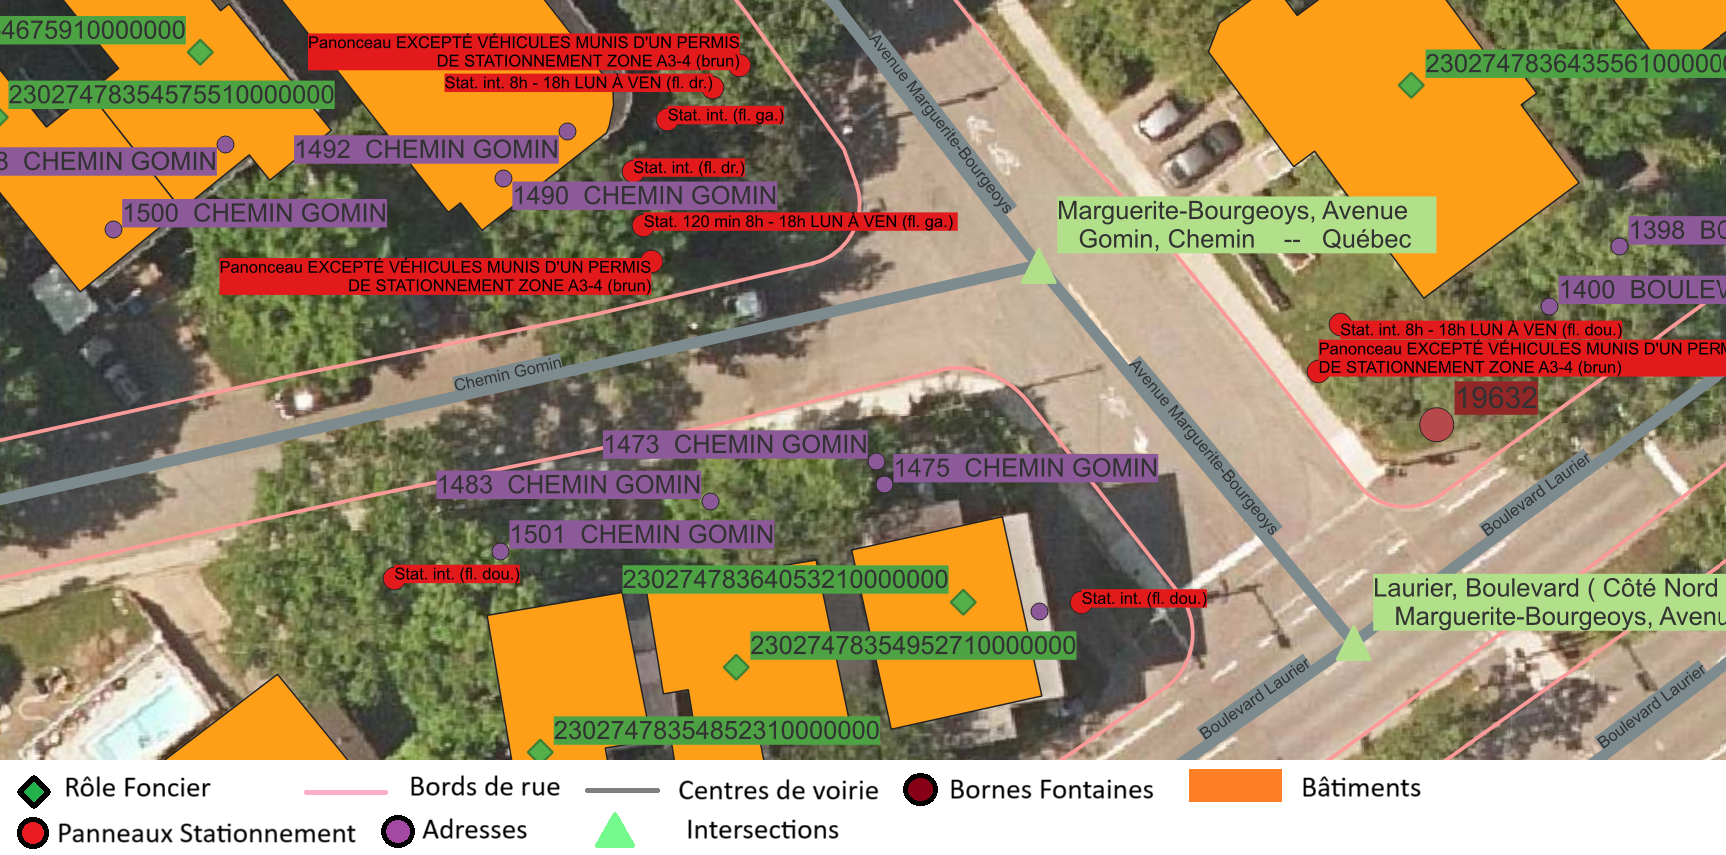
\includegraphics[width=1.0\textwidth]{images/donnees_disponible_Laurier_legende_v2.png}
        \caption{Données linéaires disponibles}
        \label{fig:donnes_panneaux_Laurier}
        \end{subfigure} \\
        \begin{subfigure}{\linewidth}
          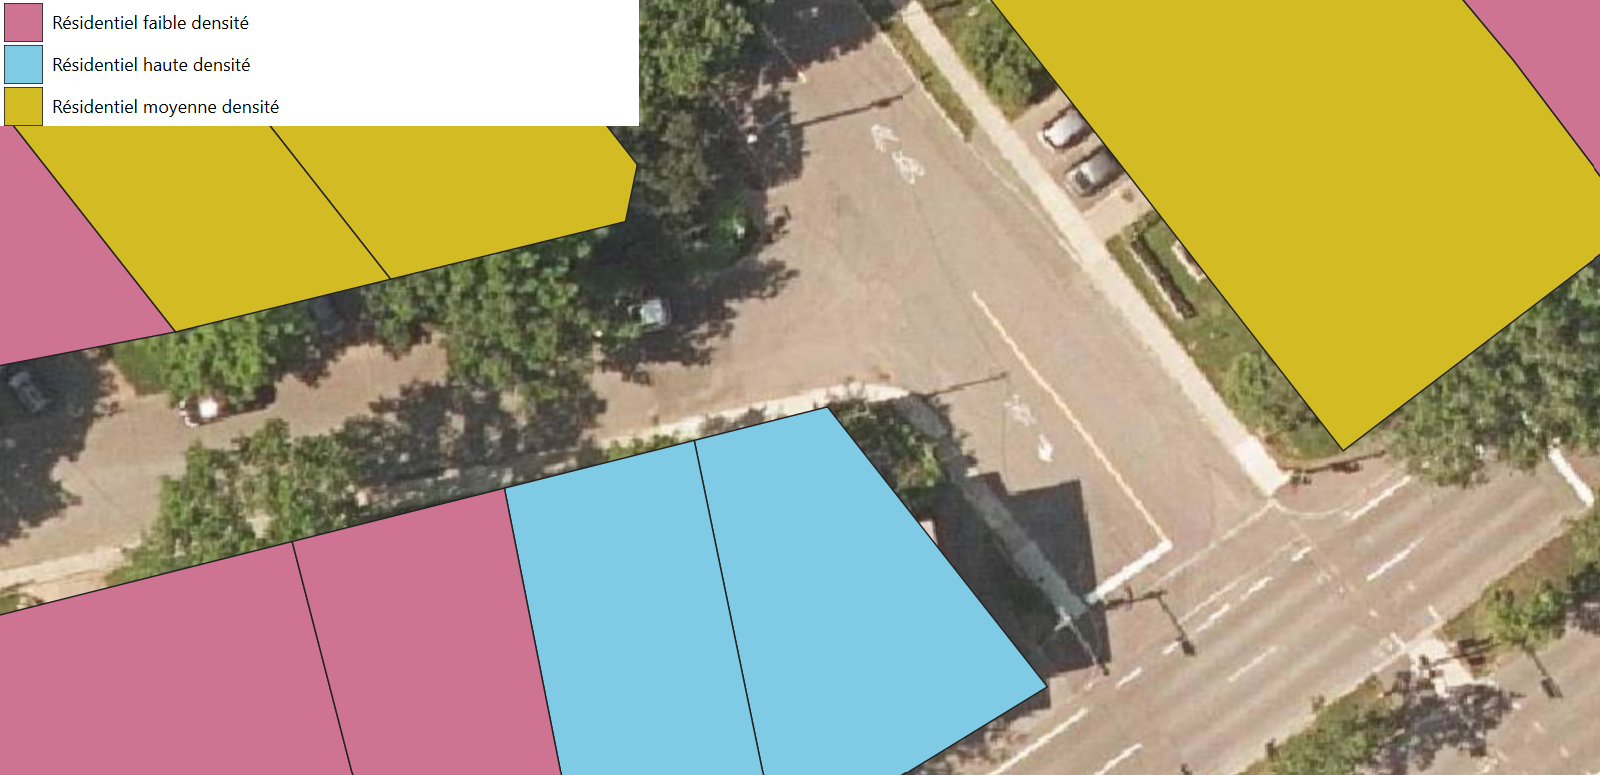
\includegraphics[width=1.0\textwidth]{images/utilisation_sols_Laurier_v2.png}
        \caption{Données polygonales disponibles}
        \label{fig:donnes_polygone_panneaux_Laurier}
        \end{subfigure}
        \caption{Données disponibles intersection Laurier}
      \end{figure}

      \FloatBarrier
    \subsubsection{Illustration - Cas 2: Coin de la Canardières - Desroches}
    Les figures \ref{fig:donnes_panneaux_Desroches} et \ref{fig:donnes_polygone_panneaux_Desroches} illustrent les mêmes données à un autre coin de rue. Ici, la localisation des panneaux porte encore plus à confusion puisque les panneaux de 2 tronçons de rue sont quasiment superposés. Il sera donc difficile d'assigner les panneaux aux bords de rues automatiquement lorsque ces derniers sont aux abords des intersections.
      \begin{figure}[ht]
        \centering
        \begin{subfigure}{\linewidth}
          \centering
          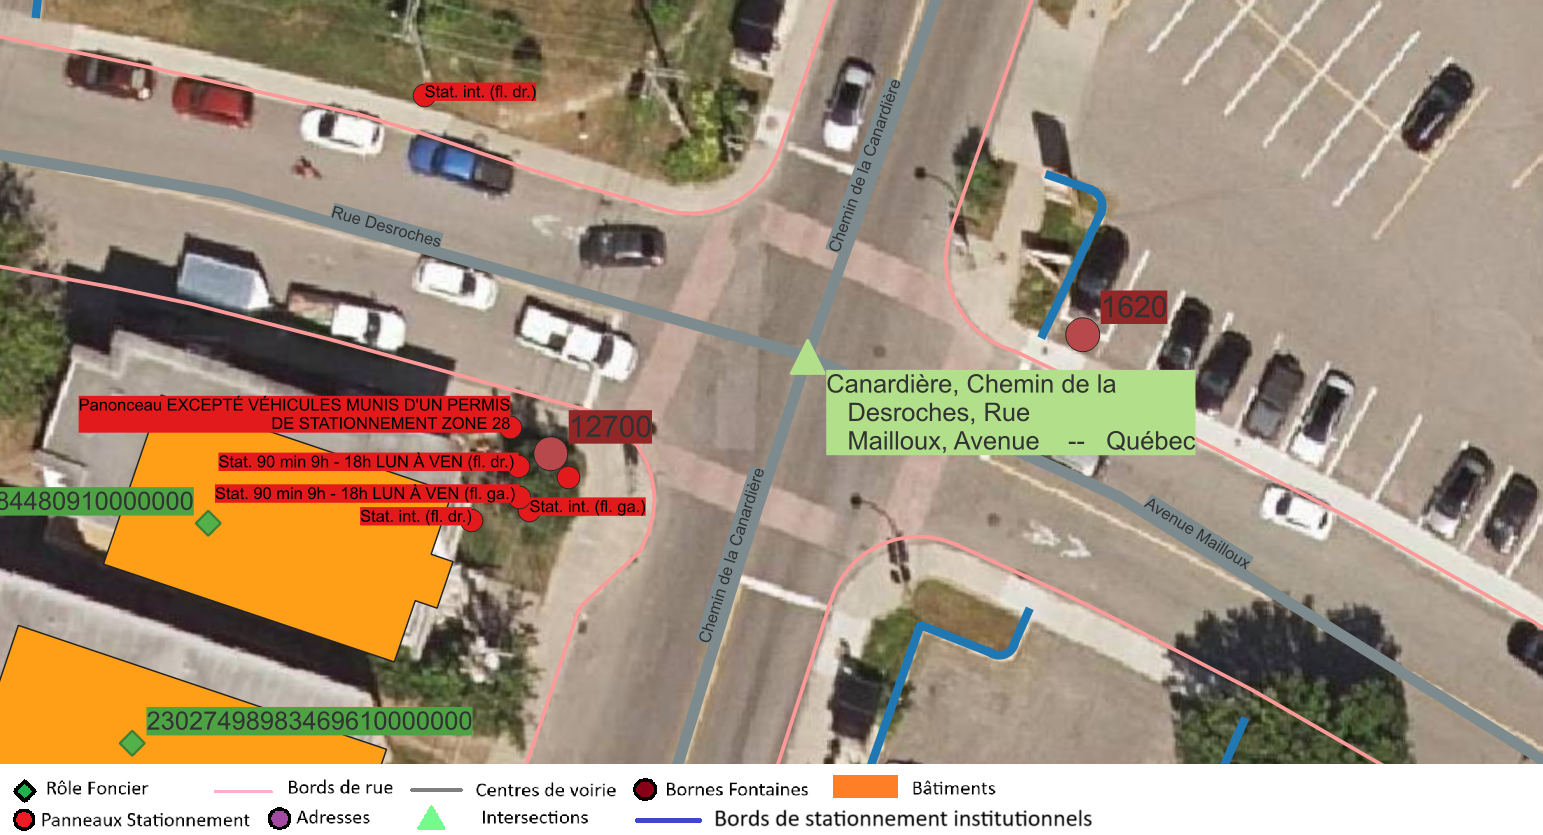
\includegraphics[width=0.8\textwidth]{images/donnees_disponible_Desroches_legende_v2.png}
        \caption{Données linéaires disponibles}
        \label{fig:donnes_panneaux_Desroches}
        \end{subfigure} \\
        \begin{subfigure}{\linewidth}
          \centering
          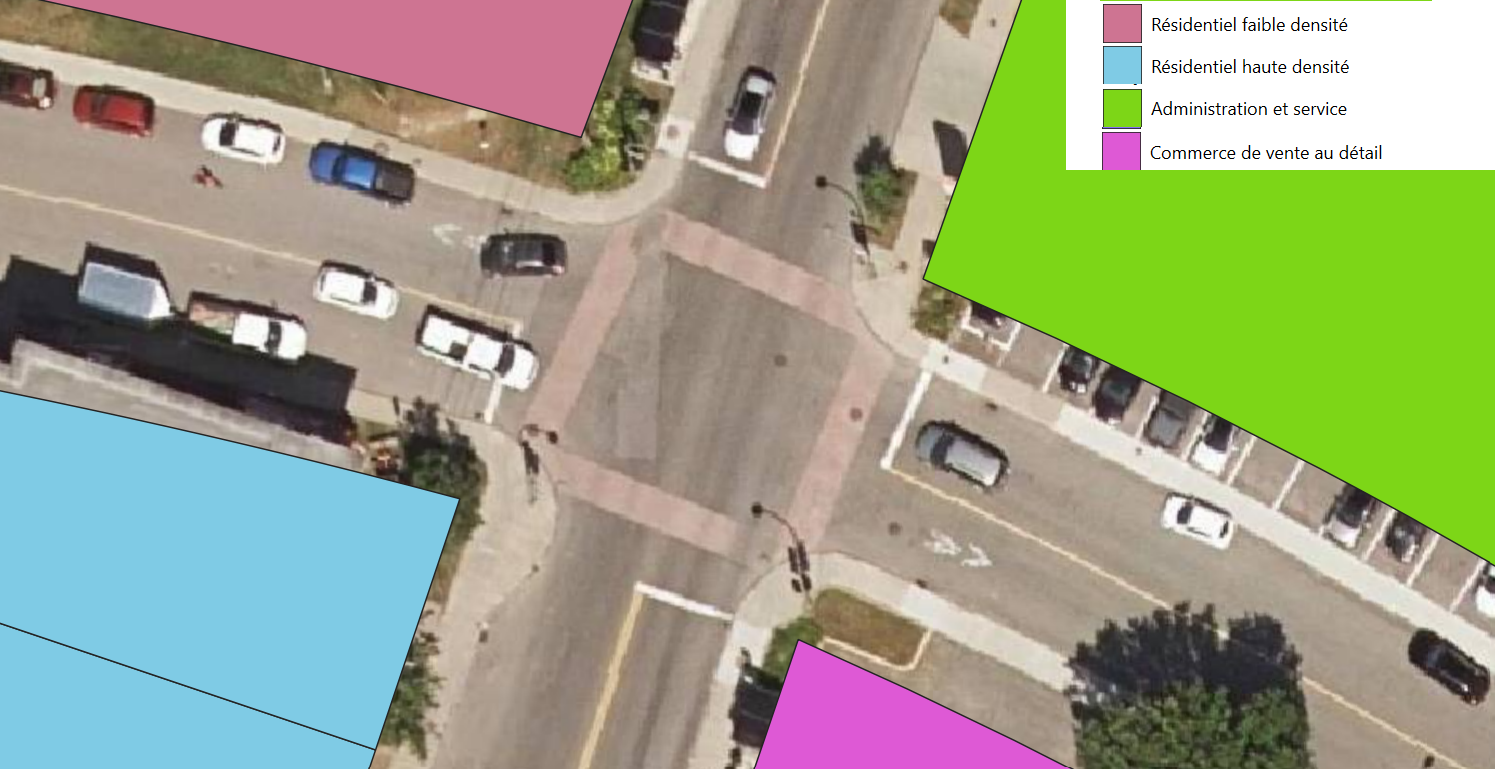
\includegraphics[width=0.8\textwidth]{images/utilisation_sols_Desroches_v2.png}
        \caption{Données polygonales disponibles}
        \label{fig:donnes_polygone_panneaux_Desroches}
        \end{subfigure}
        \caption{Données disponibles intersection Desroches / De la Canardière}
      \end{figure}
    
  \subsection{Entrainement d'apprentissage Machine}
    Plusieurs ensembles de données ont été créés pour la détection de places ouvertes dans un stationnement. Plus récemment, un ensemble de données annotées a été créé pour 
  \subsection{Enquête OD}
  \subsection{Imagerie Aérienne}
  \subsection{Rôle Foncier}
  \subsection{Recensement}
  
\section{Méthode d'inventaire sur rue}
  \subsection{Prétraitement des données}
    \subsubsection{Panneaux de stationnement}
      \subsubsection{Lisibilité Machine}
        Les panneaux ne sont pas classifiés de manière à être facilement lisibles par machine. Aucun index des panneaux de stationnement n'existe à la connaissance de l'auteur. Une classification semi-automatisée en isolant certains morceaux de chaînes de caractères a donc été créée pour rendre les panneaux de stationnement compatibles avec la structure de base de données énoncée dans \textcite{Bourdeau:MethodologieAnalyse:2014} et \textcite{Morency:DeveloppementMise:2022}. Le tableau \ref{tab:donnees_requises} liste les champs requis pour définir la fonction d'un panneau de stationnement:
        \LTcapwidth=\textwidth

        \begin{longtable}{p{0.15 \linewidth}  l p{0.5\linewidth} l  }
          \hline
          Champs & Type & Description & Valeur possibles \\
          \hline
          \endhead
          \hline
          \endfoot
          \hline
          \caption{Champs requis dans la base de données de stationnement}
          \label{tab:donnees_requises}
          \endlastfoot
          DUREE \_MAX\_ MINUTES & Entier & Durée maximale de stationnement & 0-120 \\
          TYPE\_1 & Entier & Clientèle spécifique de ce panneau & 0-11\\
          TYPE\_2 & Entier & Clientèle spécifique de ce panneau & 0-11\\
          ANNUEL & Booléen & Règlementation applicable à l'année & Vrai-Faux \\
          Date\_debut\_1 & Entier &  Date d'entrée en vigueur de la règlementation & 0-365\\
          Date\_fin\_1 & Entier & Date de fin de la règlementation & 0-365 \\
          Date\_debut\_2 & Entier & Date d'entrée en vigueur de la règlementation & 0-365 \\
          Date\_fin\_2 & Entier & Date de fin de la règlementation & 0-365 \\
          Q & Booléen & Règlementation applicable de manière quotidienne & Vrai - Faux \\
          Q\_d\_1 & Float & Heure d'entrée en vigueur de la règlementation & 0-24 \\
          Q\_f\_1 & Float & Heure de fin de la règlementation & 0-24\\
          Q\_d\_2 & Float & Heure de début de la deuxième période de validité de la règlementation 0-24\\
          LU & Booléen & Règlementation applicable un lundi (Q est nécessairement faux) & Vrai - Faux \\
          LU\_debut\_1 & Float & Heure d'entrée en vigueur de la règlementation & 0-24\\
          LU\_fin\_1 & Float & Heure d'arrêt de la règlementation & 0-24\\
          LU\_debut\_2 & Float & Deuxième Heure d'entrée en vigueur de la règlementation & 0-24\\
          LU\_fin\_2 & Float & Deuxième Heure d'arrêt de la règlementation & 0-24 \\
          MA & Booléen & Règlementation applicable un mardi (Q est nécessairement faux) & Vrai - Faux \\
          MA\_debut\_1 & Float & Heure d'entrée en vigueur de la règlementation & 0-24\\
          MA\_fin\_1 & Float & Heure d'arrêt de la règlementation & 0-24\\
          MA\_debut\_2 & Float & Deuxième Heure d'entrée en vigueur de la règlementation & 0-24\\
          MA\_fin\_2 & Float & Deuxième Heure d'arrêt de la règlementation & 0-24 \\
          ME & Booléen & Règlementation applicable un jeudi (Q est nécessairement faux) & Vrai - Faux \\
          ME\_debut\_1 & Float & Heure d'entrée en vigueur de la règlementation & 0-24\\
          ME\_fin\_1 & Float & Heure d'arrêt de la règlementation & 0-24\\
          ME\_debut\_2 & Float & Deuxième Heure d'entrée en vigueur de la règlementation & 0-24\\
          ME\_fin\_2 & Float & Deuxième Heure d'arrêt de la règlementation & 0-24 \\
          JE & Booléen & Règlementation applicable un jeudi (Q est nécessairement faux) & Vrai - Faux \\
          JE\_debut\_1 & Float & Heure d'entrée en vigueur de la règlementation & 0-24\\
          JE\_fin\_1 & Float & Heure d'arrêt de la règlementation & 0-24\\
          JE\_debut\_2 & Float & Deuxième Heure d'entrée en vigueur de la règlementation & 0-24\\
          JE\_fin\_2 & Float & Deuxième Heure d'arrêt de la règlementation & 0-24 \\
          VE & Booléen & Règlementation applicable un vendredi (Q est nécessairement faux) & Vrai - Faux\\
          VE\_debut\_1 & Float & Heure d'entrée en vigueur de la règlementation & 0-24\\
          VE\_fin\_1 & Float & Heure d'arrêt de la règlementation & 0-24\\
          VE\_debut\_2 & Float & Deuxième Heure d'entrée en vigueur de la règlementation & 0-24\\
          VE\_fin\_2 & Float & Deuxième Heure d'arrêt de la règlementation & 0-24 \\
          SA & Booléen & Règlementation applicable un samedi (Q est nécessairement faux) & Vrai - Faux \\
          SA\_debut\_1 & Float & Heure d'entrée en vigueur de la règlementation & 0-24\\
          SA\_fin\_1 & Float & Heure d'arrêt de la règlementation & 0-24\\
          SA\_debut\_2 & Float & Deuxième Heure d'entrée en vigueur de la règlementation & 0-24\\
          SA\_fin\_2 & Float & Deuxième Heure d'arrêt de la règlementation & 0-24 \\
          DI & Booléen & Règlementation applicable un samedi (Q est nécessairement faux) & Vrai - Faux \\
          DI\_debut\_1 & Float & Heure d'entrée en vigueur de la règlementation & 0-24\\
          DI\_fin\_1 & Float & Heure d'arrêt de la règlementation & 0-24\\
          DI\_debut\_2 & Float & Deuxième Heure d'entrée en vigueur de la règlementation & 0-24\\
          DI\_fin\_2 & Float & Deuxième Heure d'arrêt de la règlementation & 0-24 \\  
        \end{longtable}

      \FloatBarrier
      \subsubsection{Agrégation spatiale de plusieurs panneaux à un même endroit et association contextuelle}
    \subsubsection{Bords de rue}
    \subsubsection{Imagerie aérienne}
  \subsection{Conversion à une capacité de stationnement temporellement et spatiallement définie}
\section{Méthode d'inventaire hors rue basée sur les codes d'urbanisme}\label{sec:meth_urb_based_inventory}
    \subsection{Usages envisagés pour l'inventaire de stationnement}
    Plusieurs usages sont envisagés pour la base de données de stationnement. Il est important de les expliciter puisque cela sera la base pour l'établissement de requis pour la structure des données. Les usages envisagés sont donc les suivants:
    \begin{itemize}
        \item Étude d'accessibilité d'une place de stationnement à un lieu donnée (requiert que les places soient explicitées individuellement)
        \item Estimation du nombre de places de stationnement pour une destination précise
        \item Estimation du nombre de places de stationnement dans une zone d'analyse
        \item Analyse économétrique de l'effet de la tarification ou de la variation de l'offre sur les comportements de mobilité.
        \item Estimation de la surface minéralisée pour l'entreposage des voitures pour l'application d'écofiscalité   
    \end{itemize}
    Basé sur ces cas d'usage envisagés, la situation idéale serait d'avoir une base de données complètement désagrégée qui liste chaque place de stationnement. A minima, l'information doit être disponible au niveau du lot cadastral. D'autre part, il doit être possible d'encoder les informations relatives à la tarification de l'espace, le nombre disponible par lot , pour permettre d'appliquer des mesures d'écofiscalité. Il doit être possible d'agréger ces mesures au niveau à des zones d'analyse de déplacement pour faire des analyses sur la capacité de stationnement dans une zone dans un modèle de transport. \par
    Ultimement, l'ensemble de ces requis soulève la nécessité d'une base de donnée personnalisée. En effet, dans le cas d'un inventaire basé sur la règlementation, \ac{OSM} est mal adapté puisqu'il requiert la localisation précise des places ce qui n'est pas nécessairement faisable. D'autre part, cela ne lie pas le stationnement à un identifiant qui permet à une entité gouvernementale d'appliquer cette fiscalité. Idéalement, la base de données serait capable d'exporter un format importable dans \ac{OSM} pour mettre à jour les données ouvertes au public.
    \subsection{Choix d'une unité d'inventaire}
    Idéalement, il serait possible d'avoir la localisation précise de chaque place de stationnement. Cela permettrait de déterminer l'accessibilité aux destinations pour divers niveaux d'achalandage et choix de stationnement. Il est aussi nécessaire que les places soient agrégées par lot cadastral pour que les municipalités puissent appliquer des mesures d'écofiscalité et distribuer les places de stationnement aux divers comptes de taxes sur un même lot. Finalement, l'utilisation du lot cadastral est pertinente comme unité d'agrégation puisque que les requis sont souvent applicables à un lot qui à la construction aura des usages relativement bien définis. L
    \subsection{Proposition de base de données}
    La figure \ref{fig:offstreet_db_erd} montre la structure de la base de données utilisée pour l'estimation de l'offre de stationnement. 
    \begin{landscape}
    \begin{figure}
        \centering
        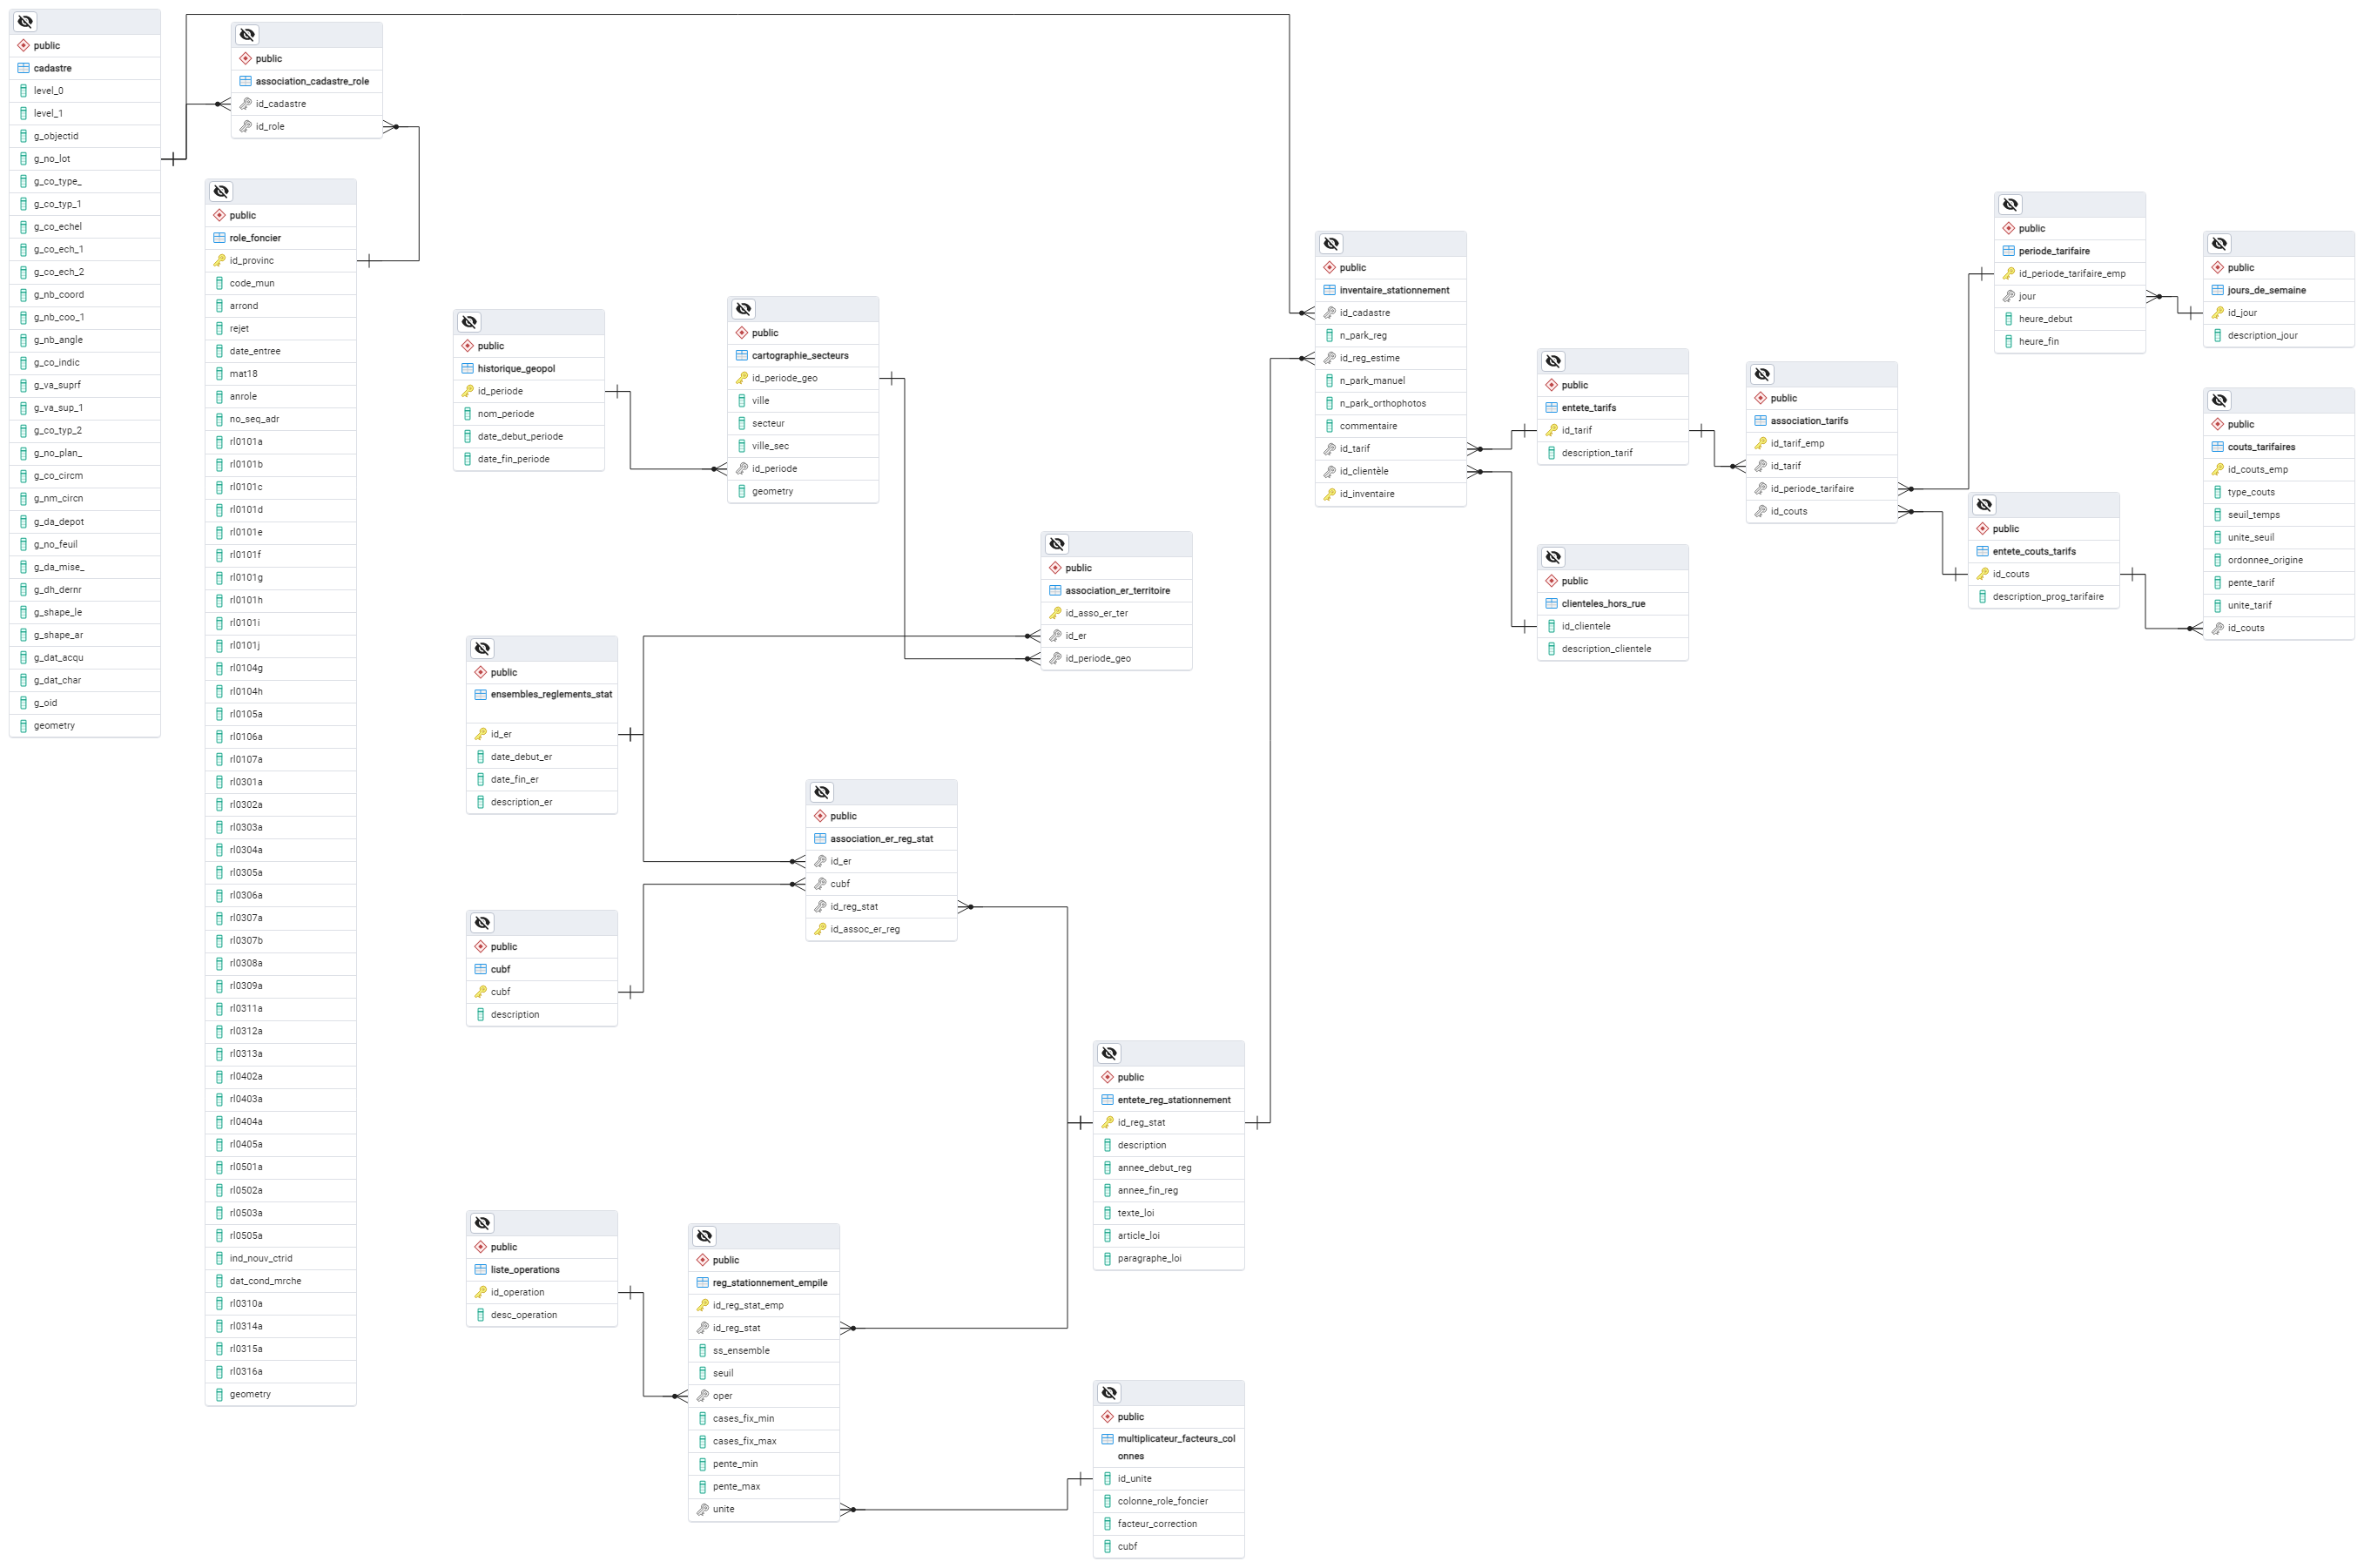
\includegraphics[width = 0.85\linewidth]{images/structure_base_de_donnee.png}
        \caption{Diagramme entité association de la base de données}\label{fig:offstreet_db_erd}
    \end{figure}
    \end{landscape}
    La base de données est implémentée dans PostgreSQL avec PostGIS pour pouvoir gérer les données spatiales du rôle foncier, du cadastre ainsi que de la division géopolitique du territoire.\par
    
    \subsubsection{Données sortantes}
    La table \underline{inventaire\_stationnement} contient l'inventaire de stationnement. La table laisse la possibilité d'avoir plusieurs estimations par lot cadastral. Ainsi, l'usager peut utiliser une estimation règlementaire, entrer une valeur manuellement ou utiliser une méthode d'estimation basée sur les orthophotos. D'autre part, des identifiants de clientèle et de tarif sont mis en place. On pourrait ainsi avoir un cas où sur un même lot cadastral il y a plusieurs stationnements (par exemple, employés, résidents, clients de commerces) ayant des modalités d'accès différentes. Chaque stationnement aurait alors un identifiant de clientèle et un identifiant de tarif. Une clé primaire est mise en place pour chaque stationnement sous la forme de la colonne id\_inventaire. Le champ id\_reg\_estime permet d'identifier le règlement d'urbanisme utilisé pour définir l'offre de stationnement estimée basé sur les règlements d'urbanisme. Cette valeur correspond à id\_reg\_stat dans la table entete\_reg\_stationnement qui sera présentée à la prochaine section.\par
    La table \underline{entete\_tarifs} est la table contenant une description et une clé primaire d'identifiant de tarifs vers laquelle pointe la table d’inventaire. La table \underline{association\_tarifs} joint une période tarifaire, un tarif et l'identifiant de tarif. La table \underline{periode\_tarifaire} permet de définir des périodes de validité. Chaque période tarifaire a un identifiant unique, un identifiant de jours, une heure de début et une heure de fin. \par
    Les tarifs ont chacun un entête avec un identifiant et une description entreposés dans la table \underline{entete\_couts\_tarifs}. La table \underline{couts\_tarifaires} contient les données de tarification. La structure a été ainsi faite pour permettre plusieurs types de tarification en fonction de l'heure de la journée et une progression de la tarification. Les champs de la table sont type\_couts qui définit s'il s'agit d'un abonnement un paiement à l'entrée ou un paiement en sortie. Le champ seuil\_temps et unite\_seuil définissent un seuil au-delà duquel le tarif s'applique. Les champs ordonnee\_origine, pente\_tarif, unite\_tarif définissent l'ordonnée à l'origine, la pente et l'unité à fournir entrée pour obtenir le prix du stationnement.\par
    Pour conclure, la table \underline{clienteles\_hors\_rue} définit l'association entre le type de clientèle et l'entier enregistré dans la table \underline{inventaire\_stationnement}. Les valeurs possibles envisagées sont listées au tableau \ref{tab:clienteles_hors_rue}.
    \begin{table}
    \centering
    \begin{tabular}{l l}
    \hline
    id\_clientèle & Description clientèle\\ \hline
    0& Automobiles - Propriétaire et Visiteurs Autorisés \\
    1 & Automobiles - Propriétaires Seulement \\
    2 & Automobiles - Clients \\
    3 & Automobiles - Employés seulement \\
    4 & Automobiles - Véhicules autorisés \\
    5 & Automobiles - Vignettes résidents \\
    6 & Automobiles - Vignettes Autres \\
    7 & Automobiles - Tous\\ \hline
    \end{tabular}
    \caption{Entrées dans la table \underline{clienteles\_hors\_rue}}\label{tab:clienteles_hors_rue}
    \end{table}
    \FloatBarrier
    La figure \ref{fig:offstreet_db_erd_output} montre le détail de la base de données discutée dans cette section. Cette structure permet de séparer les places disponibles aux différentes clientèles de manière extensible pour chaque lot et de répertorier des structures de tarification complexe au besoin.
    \begin{figure}[!h]
        \centering
        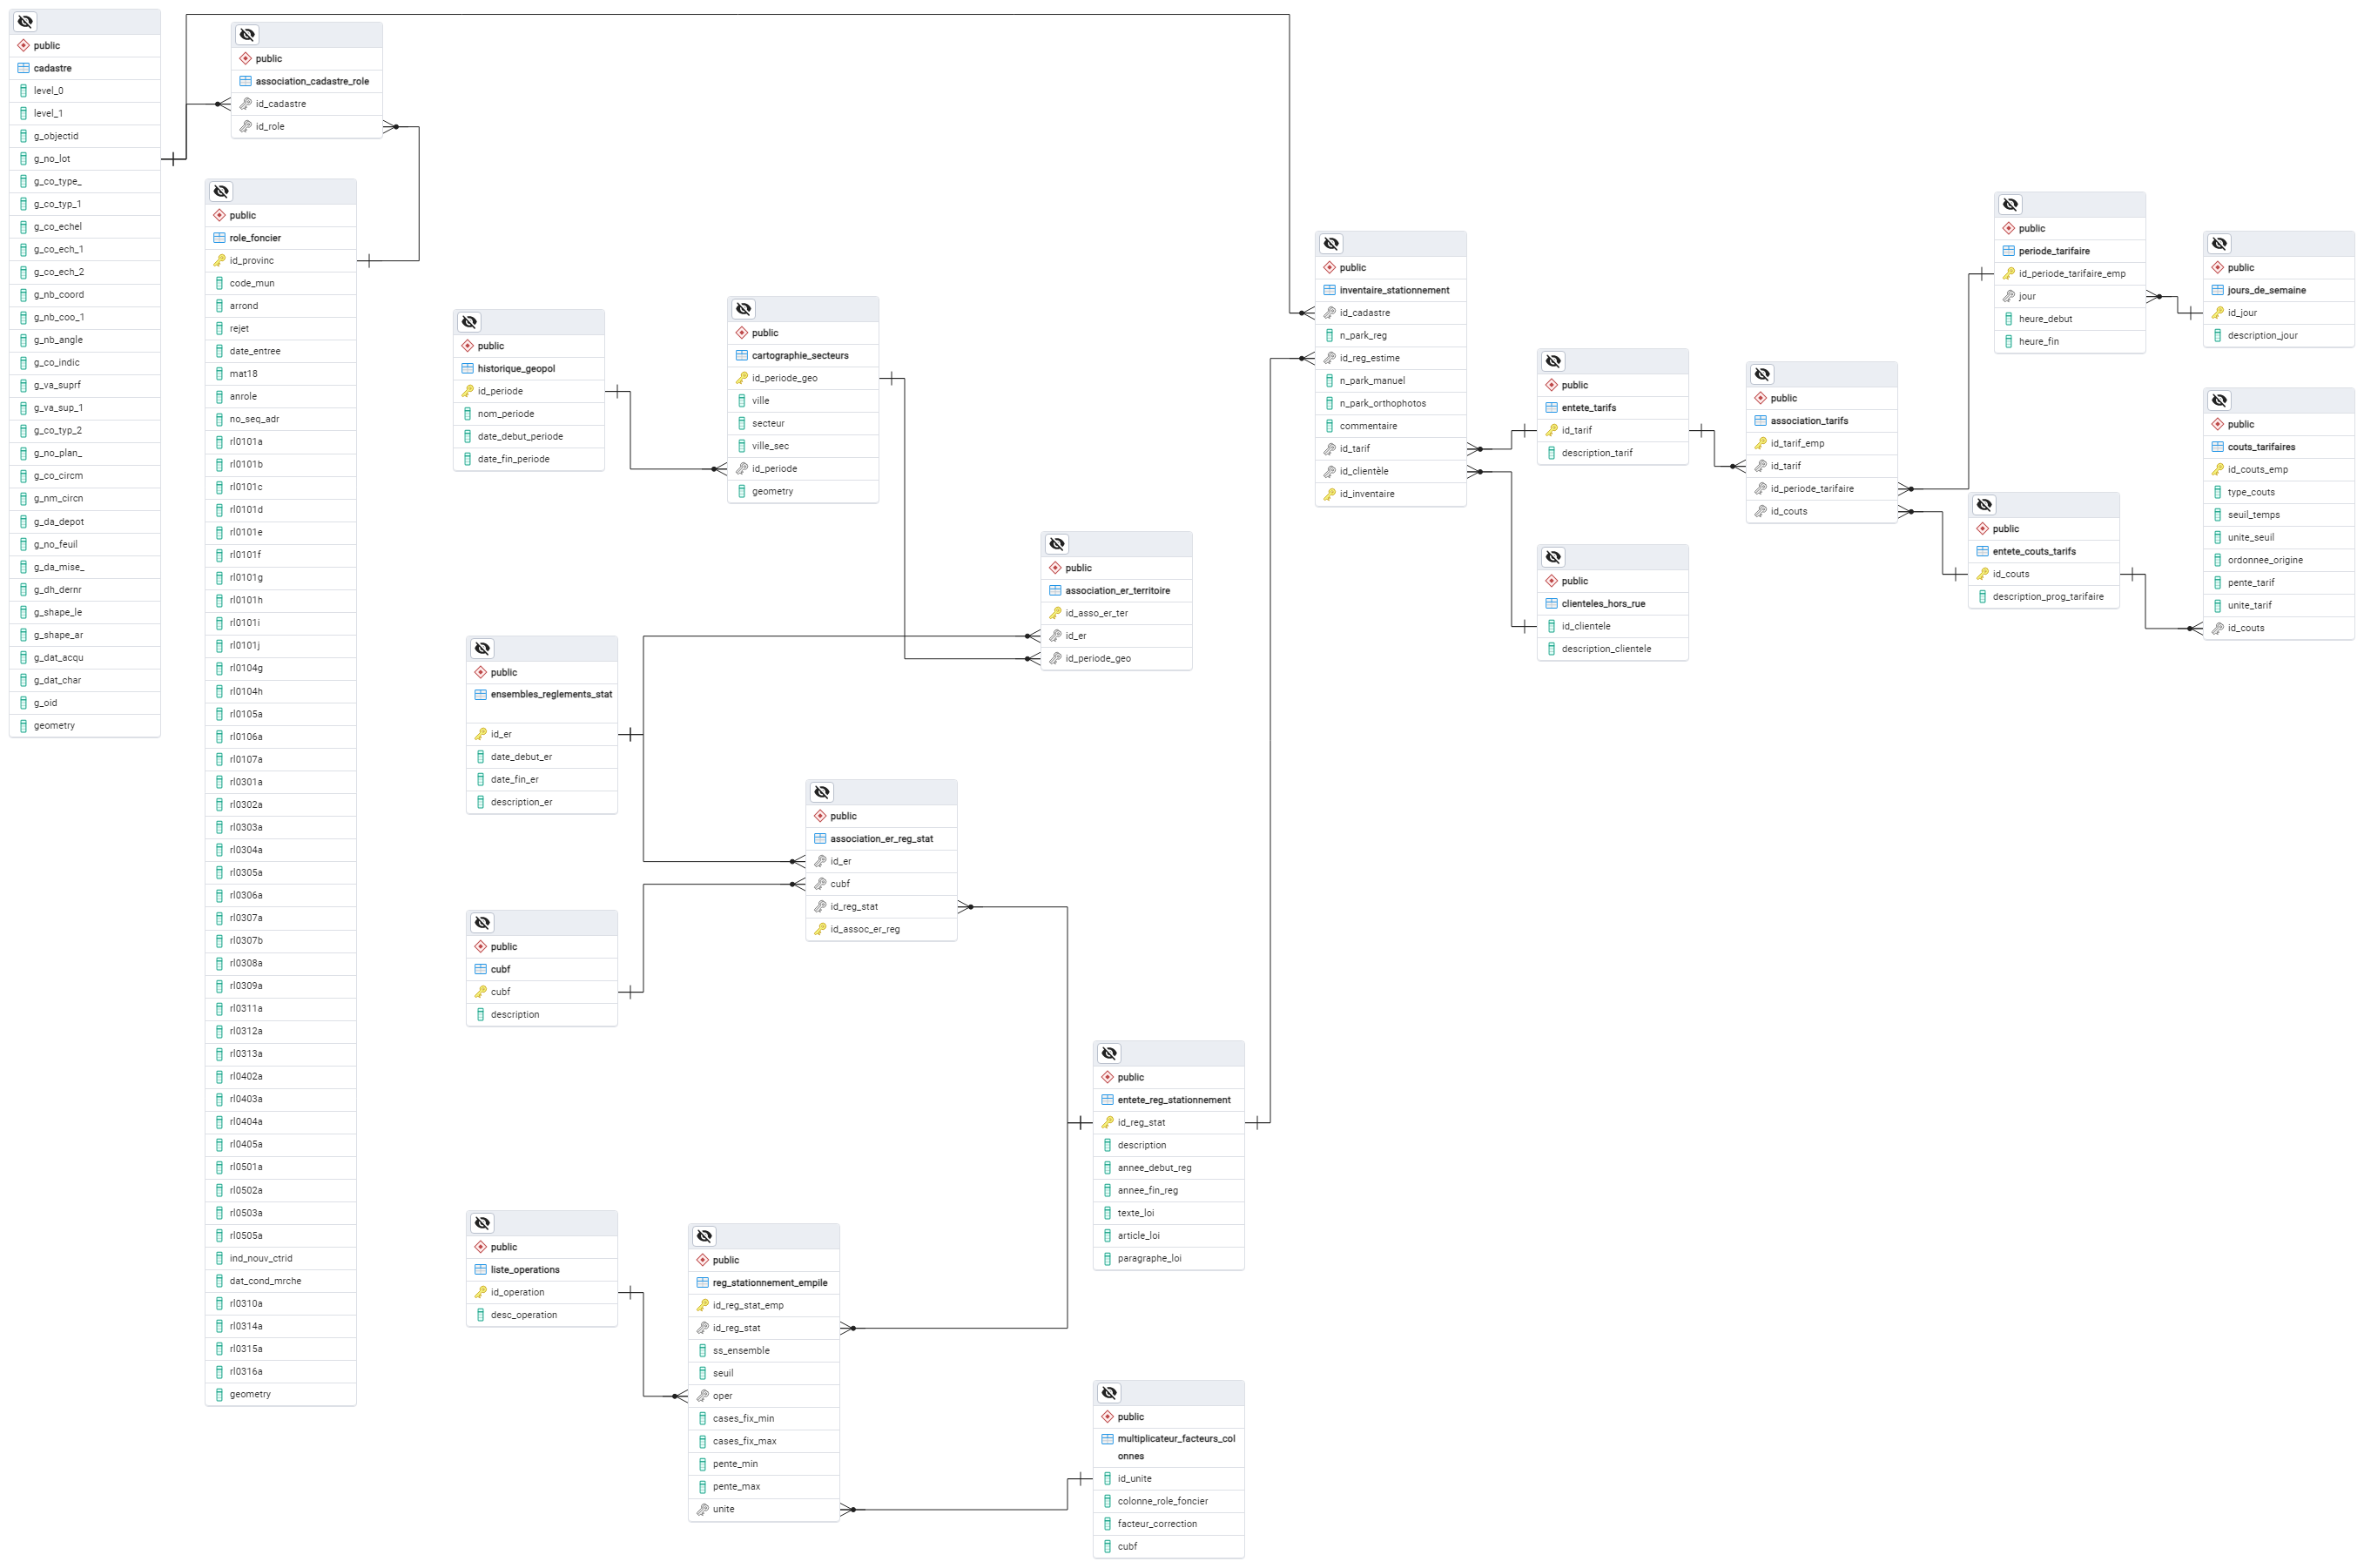
\includegraphics[trim={50cm 35cm 0 7cm}, clip, width=14cm]{images/structure_base_de_donnee.png}
        \caption{Structure de données en sortie de procédure de calcul}\label{fig:offstreet_db_erd_output}
    \end{figure}
    \FloatBarrier

    
    \subsubsection{Représentation des limites géopolitiques au travers du temps} 
    Une composante de la méthodologie proposée est d'utiliser les règlements d'urbanisme pour proposée une estimation de la capacité de stationnement basé sur les règlements d'urbanisme. Cette section présentera la manière dont la règlementation est représentée dans la base de données.
    \paragraph{Historique géopolitique} L'historique géo politique de la ville est représenté au moyen de deux tables: \underline{historique\_geopol} et \underline{cartographie\_secteurs}. \underline{historique\_geopol} représente les grandes périodes où le territoire a été stable. Dans le cadre de ce mémoire, 6 grandes périodes ont été identifiées basé sur \textcite{VilledeQuebec:ReperesChronologique:} et \textcite{ElectionsQuebec:AtlasHistorique:2021}. Elles sont listées au tableau \ref{tab:histo_geopol}
    \begin{table}
    \centering
    \begin{tabular}{c p{5cm} c c}
    \hline
    \makecell{Identifiant\\ id\_periode} & \makecell[l]{Nom \\ nom\_periode} & \makecell{Année début \\ date\_debut\_periode} & \makecell{Année fin \\ date\_fin\_periode}\\ \hline
    1 & Fondation - 1970 &  S.V. & 1970 \\
    3 & Duberger, Saules et Neufchâtel fusion Québec & 1971 & 1975 \\
    4 & Fusions Charlesbourg & 1976 & 1994 \\
    5 & Inauguration VQZ-3 & 1995 & 1996 \\
    6 & Abrogation Zone Prioritaire Ville de Québec & 1997 & 2009 \\
    7 & Harmonisation & 2010 & S.V.\\ \hline
    \end{tabular}
    \caption{Valeurs dans l'historique géopolitique utilisé dans le cadre de ce mémoire}\label{tab:histo_geopol}
    \end{table}
    \FloatBarrier
    La table \underline{cartographie\_secteurs} contient les délimitations des secteurs pour chacune des périodes. Les champs sont les suivants :id\_periode\_geo est l'identifiant primaire, id\_periode est la clé qui référence à la table \underline{historique\_geopol}, le champ ville contient le nom de la ville, le champ secteur est un nom de secteur, et le champ ville\_sec est une concaténation des deux champs précédents. En plus de l'information tabulaire, les limites géographiques des secteurs sont entreposées dans cette table. \par
    La figure \ref{fig:offstreet_db_erd_history} montre le détail de la section de base de donnée montrant l'évolution des variations géopolitiques du territoire.
    \begin{figure}
        \centering
        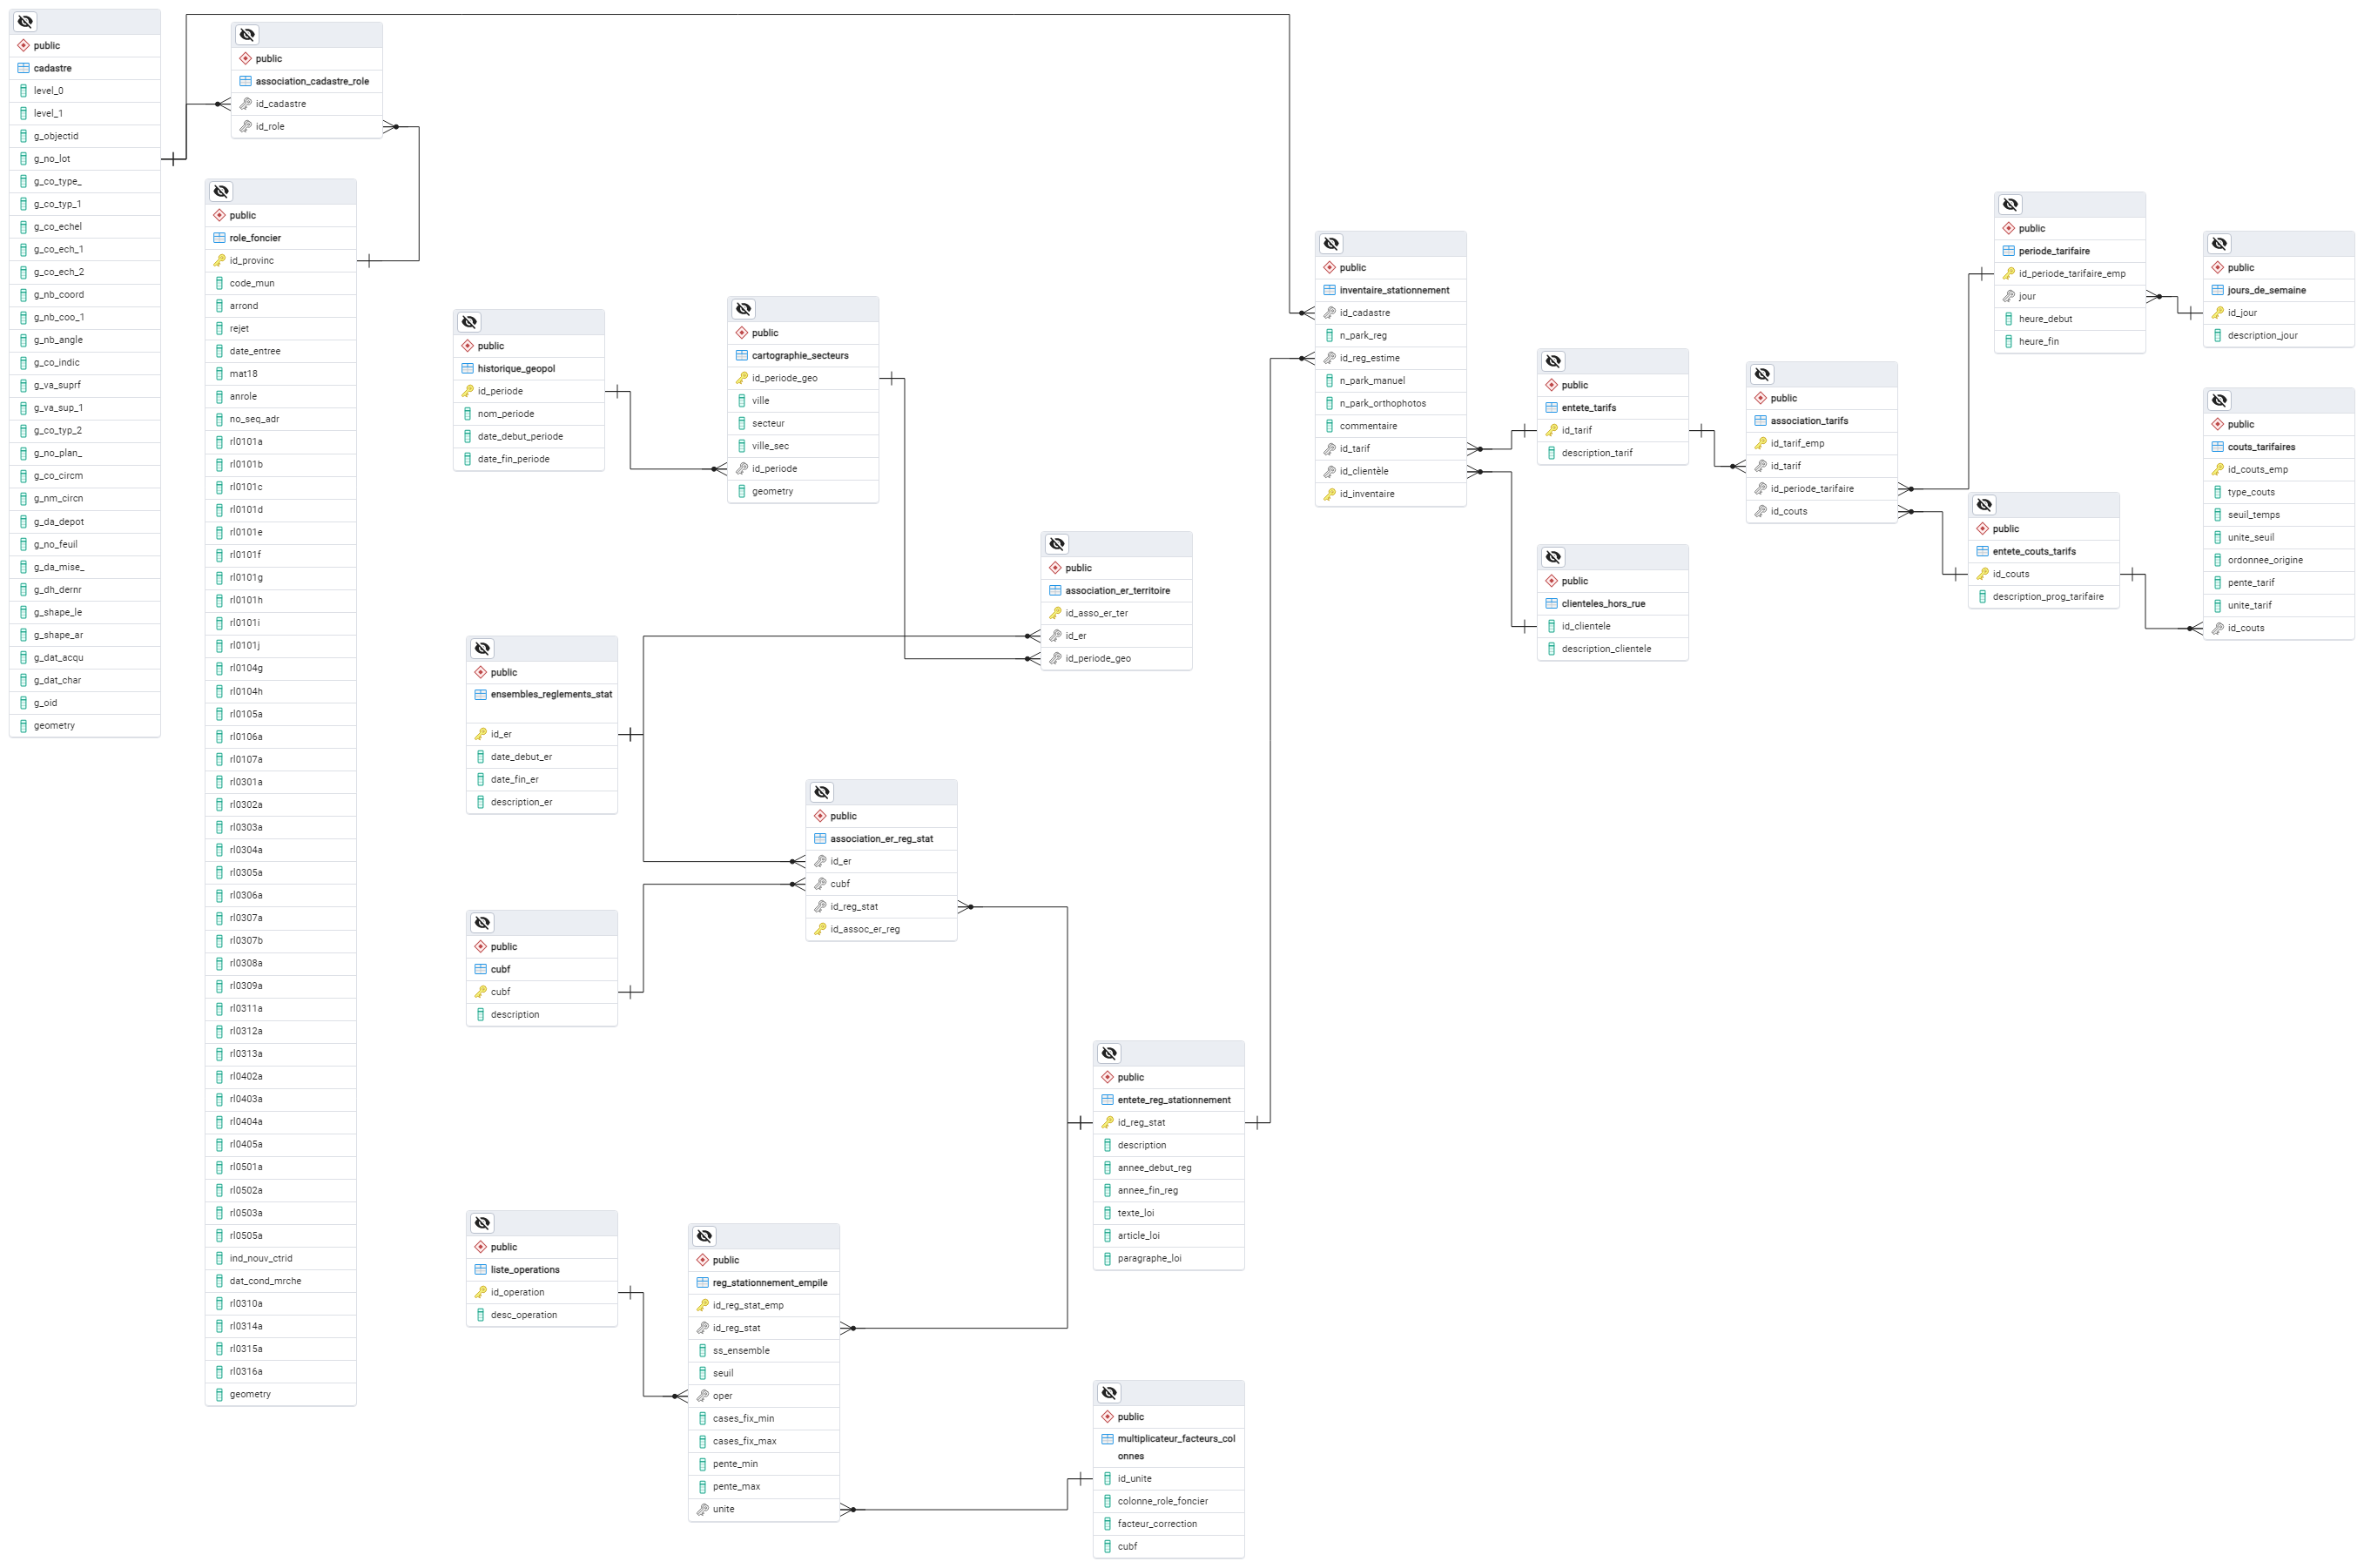
\includegraphics[trim={18cm 40cm 60cm 12cm}, clip, width=8cm]{images/structure_base_de_donnee.png}
        \caption{Structure de données pour l'historique géopolitique}\label{fig:offstreet_db_erd_history}
    \end{figure}
    \FloatBarrier
    
    \subsubsection{Représentation de règlements individuels} 
    Les règlements sont ensuite définis individuellement dans la table \underline{entete\_reg\_stationnement}. Cette table contient les champs suivants: id\_reg\_stat est l'identifiant unique pour chaque règlement, le champ description est une description textuelle issue du règlement décrivant l'usage du sol associé au règlement, annee\_debut\_reg contient la date d'entrée en vigueur du règlement, annee\_fin\_reg contient l'année d'abrogation du règlement, texte\_loi, article\_loi et paragraphe\_loi contiennent la provenance du règlement et ville indique la ville qui a issue le règlement. La description du nombre de places requises est entreposée dans la table \underline{reg\_stat\_empile}. Les champs de la table sont les suivants: id\_reg\_stat\_emp est l'identifiant unique pour la table, id\_reg\_stat permet d'unifier plusieurs lignes de la table à un même règlement. Cette stratégie permet de représenter des règlements complexes sur plusieurs lignes de la base de données. La colonne ss\_ensemble permet de définir des sous-ensembles au règlement, ce champ permet de séparer des conditions complexes.  Le champ seuil définit une borne inférieure à son applicabilité. L'unité pour le seuil est la même que celle utilisée en entrée des équations linéaires définies dans les autres champs de la même ligne. Le champ oper contient l'opération à appliquer à la ligne. Toutes les lignes sauf la première devraient avoir une valeur pour ce champ. Les champs cases\_fix\_min et cases\_fix\_max définissent l'abscisse à l'ordonnée, pente\_min et pente\_max définissent la pente, et unite définit l'unité utilisée. Le champ unité et un entier et est la clé primaire pour la table \underline{multiplicateur\_facteurs\_colonnes}. \par 
    Les opérations possibles sont listées dans la table liste\_operations qui a deux champs: id\_operation et desc\_operation. Les valeurs possibles sont listées au tableau \ref{tab:operations_table}.
    \begin{table}[h]
        \centering
        \begin{tabular}{cl}
             \hline
             id\_operation & desc\_operation  \\ \hline
             1 & + (absolu)\\
             2 & + (au-delà seuil >=)(obsolète)\\
             3 & ou (plus contraignant) \\
             4 & changement critère au dela seuil (>=)\\
             5 & changement critère dans centre commercial(obsolète)\\
             6 & ou simple \\ \hline
        \end{tabular}
        \caption{Opérations listées dans la table liste\_operations}
        \label{tab:operations_table}
    \end{table}
    Cette dernière contient trois 5 champs: id\_unite, colonne\_role\_foncier, facteur\_correction, cubf, desc\_unite. Le champ id\_unite est référencé par le champ unite de la table \underline{reg\_stat\_empile}, colonne role foncier donne le nom de la colonne dans le rôle foncier qui doit être utilisée dans l'équation et la comparaison au seuil, la colonne facteur correction donne la possibilité de multiplier la valeur dans la colonne du rôle foncier pour appliquer une correction. Le champ cubf permet de donner un facteur de correction différent pour différents types de \ac{CUBF}. Le champ desc\_unite donne une brève description de l'unité. Le tableau \ref{tab:unite_pertinentes_minimum_stat} donne les le contenu de la table multiplicateur\_facteur\_colonnes.\par
    \begin{table}[h]
    \centering
        \begin{tabular}{c l c c p{3cm}}
            \hline
            id\_unite & colonne\_role\_foncier & facteur\_correction & cubf & desc\_unite \\ \hline
            1 & rl0312a & 1 & S.V. & chambre\\
            2 & rl0311a & 1 & S.V. & logement \\
            4 & rl0308a & 1 & S.V. & metre carré d'étage\\
            5 & S.V. & 1 & S.V. & metre carré bureau\\
            6 & S.V. & 1 & S.V. & metre carré salle production \\
            7 & rl0302a & 1 & S.V. & metre carré terrain\\
            8 & S.V. & 1 & S.V. & siège \\
            9 & S.V. & 1 & S.V. & poste de travail \\
            10 &S.V. & 1 & S.V. & salle \\
            11 & S.V. & 1 & S.V. & lit \\
            12 & S.V. & 1 & S.V. & personne \\
            13 & S.V. & 1 & S.V. & employé \\
            14 & S.V. & 1 & S.V. & étudiant \\
            15 & S.V. & 1 & S.V. & médecin \\
            16 & S.V. & 1 & S.V. & quai \\
            17 & S.V. & 1 & S.V. & voie de service \\
            18 & S.V. & 1 & S.V. & vert \\
            19 & S.V. & 1 & S.V. & allee de pratique \\
            20 & S.V. & 1 & S.V. & plateau sportif \\ \hline
        \end{tabular}
        \caption{Unités utilisées pour codifier les codes d'urbanismes}\label{tab:unite_pertinentes_minimum_stat}
    \end{table}
    \FloatBarrier
    Les équations donnent les étapes mathématiques pour une ligne d'un règlement de stationnement sont donc données aux équations \ref{eq:x_entree}, \ref{eq:places_max} et \ref{eq:places_min} si $x_{entree} \geq seuil $.
    \begin{align}
        x_{entree} &= role\_foncier[colonne\_role\_foncier] \times facteur\_correction \label{eq:x_entree}\\
        n_{places,min} &= cases\_fix\_min + pente\_min \times x_{entree} \label{eq:places_min}\\
        n_{places,max} &= cases\_fix\_max + pente\_max \times x_{entree} \label{eq:places_max}
    \end{align}
    \clearpage
    \paragraph{Exemple 1: Clinique medicale} Admettons un règlement qui requiert 1 place par salle de consultation  plus une place par employé plus une place par médecin ou une place par 20 mètres carrés, au plus contraignant. Les entrées dans la table reg\_stat\_empile seraient telles que montrées au tableau \ref{tab:ex_reg_stat_clinique}
    \begin{table}[h]
        \centering
        \begin{tabular}{cccccccccc}
            \hline
            \rotatebox{90}{id\_emp} & \rotatebox{90}{id\_reg\_stat} & \rotatebox{90}{ss\_ensemble} & \rotatebox{90}{seuil}  & \rotatebox{90}{oper}  & \rotatebox{90}{cases\_fix\_min}   & \rotatebox{90}{cases\_fix\_max}   & \rotatebox{90}{pente\_min}    & \rotatebox{90}{pente\_max} & \rotatebox{90}{unite}    \\ \hline
            1                       & 1                             &  1                           & 0                      &  S.V.                 & 0                                 & S.V.                              & 1                             & S.V.                       & 15                       \\
            2                       & 1                             &  1                           & 0                      &  1                    & 0                                 & S.V.                              & 1                             & S.V.                       & 13                       \\
            3                       & 1                             &  1                           & 0                      &  1                    & 0                                 & S.V.                              & 1                             & S.V.                       & 10                       \\
            4                       & 1                             &  2                           & 0                      &  3                    & 0                                 & S.V.                              & 0.05                          & S.V.                       & 4                       \\ \hline
        \end{tabular}
        \caption{Exemple règlements dans la table reg\_stat\_empile pour une clinique médicale}
        \label{tab:ex_reg_stat_clinique}
    \end{table}
    \begin{figure}[h]
    \begin{subfigure}[t]{0.5\textwidth}
       \centering
       \begin{tikzpicture}[scale=0.8]
        \begin{axis}[
            xlabel={$N_{employes}$[-]},
            ylabel={$N_{médecin}$[-]},
            zlabel={$N_{places}$[-]},
            legend style={at={(0.5,1.25)},
	           anchor=north,legend columns=-1}
        ]
        \addplot3[
            surf,color = blue, faceted color=black,
        ] 
        coordinates {
        (0,0,1) (0,1,2) (0,2,3)
        
        (1,0,2) (1,1,3) (1,2,4)
        
        (2,0,3) (2,1,4) (2,2,5)
        };
        \addplot3[
            surf,color = orange, faceted color=black,
        ] 
        coordinates {
        (0,0,2) (0,1,3) (0,2,4)
        
        (1,0,3) (1,1,4) (1,2,5)
        
        (2,0,4) (2,1,5) (2,2,6)
        };
        \legend{Stat min. $n_{salles}=1$,Stat min. $n_{salles}=2$}
        \end{axis} 
        \end{tikzpicture}
        \caption{Sous ensemble 1 du règlement}
    \end{subfigure}
    ~
    \begin{subfigure}[t]{0.5\textwidth}
        \centering
        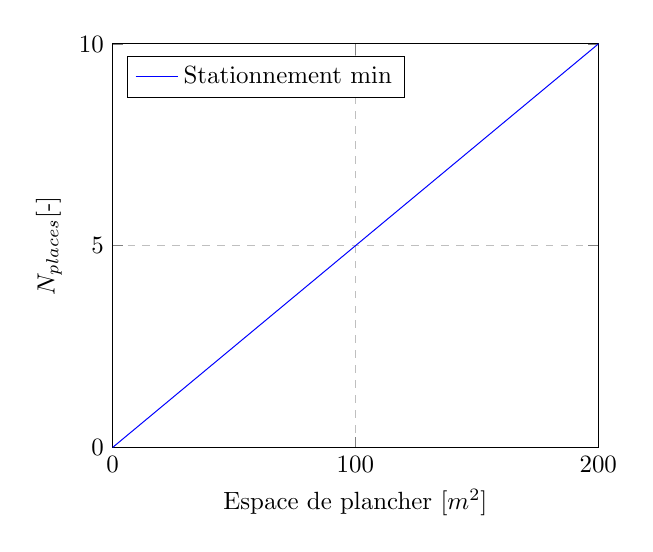
\begin{tikzpicture}[scale = 0.9]
        \begin{axis}[
            xlabel={Espace de plancher [$m^2$]},
            ylabel={$N_{places}$[-]},
            xmin=0, xmax=200,
            ymin=0, ymax=10,
            xtick={0,100,200},
            ytick={0,5,10},
                legend pos=north west,
            ymajorgrids=true,
            xmajorgrids=true,
            grid style=dashed,
            domain=0:1000, 
        ]
        \addplot[color=blue]{x/20};
        \legend{Stationnement min}
        \end{axis}
    \end{tikzpicture}
    \caption{Sous ensemble 2 du règlement}
    \end{subfigure}
    \caption{Exemple de règlement de stationnement pour une clinique médicale}
    \end{figure}
    \FloatBarrier
    \clearpage
    \paragraph{Exemple 2: Logements} Dans le cas d'un logement, les règlements changes souvent en fonction du nombre de logements au sein d'un même bâtiment. Dans ce cas hypothétique, le requis serait de une case par logement pour des bâtiments de moins de 4 logements, 1.5 cases par logement pour les bâtiments entre 4 et 7 logements et 1.25 case par logements pour tout bâtiment de 8 logements ou plus. Dans ce cas, les entrées à la table seraient telles que montrées au tableau
    \begin{table}[h]
        \centering
        \begin{tabular}{cccccccccc}
            \hline
            \rotatebox{90}{id\_emp} & \rotatebox{90}{id\_reg\_stat} & \rotatebox{90}{ss\_ensemble} & \rotatebox{90}{seuil}  & \rotatebox{90}{oper}  & \rotatebox{90}{cases\_fix\_min}   & \rotatebox{90}{cases\_fix\_max}   & \rotatebox{90}{pente\_min}    & \rotatebox{90}{pente\_max} & \rotatebox{90}{unite}    \\ \hline
            5                       & 2                             &  1                           & 0                      &  S.V.                 & 0                                 & S.V.                              & 1                             & S.V.                       & 2                       \\
            6                       & 2                             &  1                           & 4                      &  4                    & 0                                 & S.V.                              & 1.5                           & S.V.                       & 2                       \\
            7                       & 2                             &  1                           & 8&  4                    & 0                                 & S.V.                              & 1.25                          & S.V.                       & 2                       \\ \hline
        \end{tabular}
        \caption{Exemple règlements dans la table reg\_stat\_empile pour le logement}
        \label{tab:ex_reg_logement}
    \end{table}
     \begin{figure}[h]
       \centering
        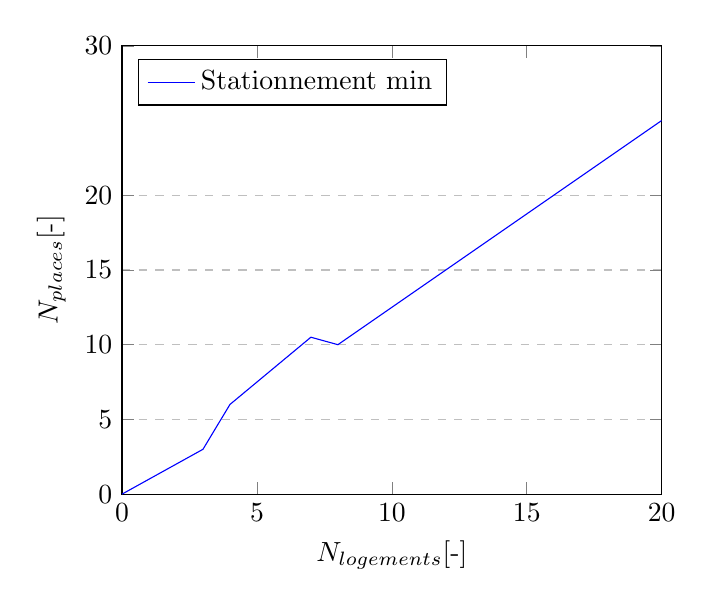
\begin{tikzpicture}[scale=1.0]
            \begin{axis}[
                xlabel={$N_{logements}$[-]},
                ylabel={$N_{places}$[-]},
                xmin=0, xmax=20,
                ymin=0, ymax=30,
                xtick={0,5,10,15,20},
                ytick={0,5,10,15,20,30},
                legend pos=north west,
                ymajorgrids=true,
                grid style=dashed,
            ]
            \addplot[
                    color=blue
                    ]
                 coordinates {
                    (0,0)(3,3)(4,6)(5,7.5)(6,9)(7,10.5)(8,10)(10,12.5)(15,18.75)(20,25)
                };
    
            \legend{Stationnement min}
            \end{axis}
        \end{tikzpicture}
    \caption{Exemple de règle de stationnement pour logement}
    \end{figure}
    \FloatBarrier
    \clearpage
    \paragraph{Exemple 3: Lieux d'assemblée} Dans le cas de lieux d'assemblée, les requis peuvent être exprimés en fonction du nombre de sièges ou en fonction de l'espace au sol. Dans notre cas hypothétique, le requis serait un minimum d'une place par 7 sièges jusqu'à 800 sièges et d'un minimum de 1 place par 9 sièges pour toute place au-delà de 800 siège. Un maximum  d'une place par 5 sièges est applicable au-delà de 500 sièges. Quand il n'y a pas de sièges, un requis d'une places par 10 mètres carrés est applicable sans maximum.
    \begin{table}[h]
        \centering
        \begin{tabular}{cccccccccc}
            \hline
            \rotatebox{90}{id\_emp} & \rotatebox{90}{id\_reg\_stat} & \rotatebox{90}{ss\_ensemble} & \rotatebox{90}{seuil}  & \rotatebox{90}{oper}  & \rotatebox{90}{cases\_fix\_min}   & \rotatebox{90}{cases\_fix\_max}   & \rotatebox{90}{pente\_min}    & \rotatebox{90}{pente\_max} & \rotatebox{90}{unite}    \\ \hline
            8                       & 3                             &  1                           & 0                      &  S.V.                 & 0                                 & S.V.                              & 0.142857                      & S.V.                       & 8                       \\
            9                       & 3                             &  1                           & 500                    &  4                    & 0                                 & 0                                 & 0.142857                      & 0.2                        & 8                       \\
            10                      & 3                             &  1                           & 800                    &  4                    & 25.396825                         & 0                                 & 0.111111                      & 0.2                        & 8                       \\
            11                      & 3                             &  2                           & 0                      &  6                    & 0                                 & S.V.                              & 0.1                           & S.V.                       & 4                       \\\hline
        \end{tabular}
        \caption{Exemple règlements dans la table reg\_stat\_empile pour un lieu d'assemblée}
        \label{tab:ex_reg_lieu_assemblee}
    \end{table}
   \begin{figure}[h]
        \begin{subfigure}[t]{0.5\textwidth}
        \centering
            \begin{tikzpicture}[scale = 0.9]
            \begin{axis}[
                xlabel={$N_{sièges}$[-]},
                ylabel={$N_{places}$[-]},
                xmin=0, xmax=1000,
                ymin=0, ymax=200,
                xtick={0,200,400,600,800,1000},
                ytick={0,50,100,150,200},
                    legend pos=north west,
                ymajorgrids=true,
                grid style=dashed,
            ]
        
            \addplot[
                color=blue
                ]
            coordinates {
            (0,0)(500,71.4285)(800,114.2856)(1000,136.507938)
            };
            \addplot[
            color = red
            ]
            coordinates{
                (500,100)(1000,200)
            };
            \legend{Stationnement min, Stationnement max}
            \end{axis}
        \end{tikzpicture}
            \caption{Avec sièges}
    \end{subfigure}
    \begin{subfigure}[t]{0.5\textwidth}
        \centering
        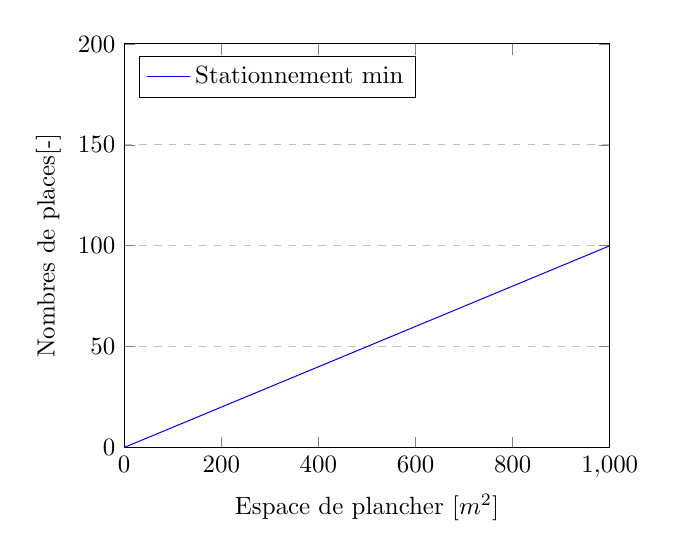
\begin{tikzpicture}[scale = 0.9]
        \begin{axis}[
            xlabel={Espace de plancher [$m^2$]},
            ylabel={Nombres de places[-]},
            xmin=0, xmax=1000,
            ymin=0, ymax=200,
            xtick={0,200,400,600,800,1000},
            ytick={0,50,100,150,200},
                legend pos=north west,
            ymajorgrids=true,
            grid style=dashed,
        ]
        \addplot[
            color=blue
            ]
        coordinates {
        (0,0)(500,50)(800,80)(1000,100)
        };
        \legend{Stationnement min}
        \end{axis}
    \end{tikzpicture}
        \caption{Sans sièges}
    \end{subfigure}
    \captionsetup{justification=centering}
\caption{Exemple de règle de stationnement pour lieux d'assemblée}
\end{figure}
    \FloatBarrier
    \subsubsection{Création d'ensembles de règlements}
    Du fait de la variation de la règlementation dans le temps, des règlements instaurés à différents moments peuvent être applicables à une même période. Pour permettre de créer un tout cohérent représentant l'état de la règlementation à un instant T à un endroit sur le territoire de l'actuelle ville de Québec. Cette section va introduire le schéma relationnel de ces ensembles de règlements. Trois tables sont crées pour assurer l'expansibilité du système: \underline{ensembles\_reglements\_stat}, \underline{cubf}, \underline{association\_er\_reg\_stat}.\par
    \underline{ensembles\_reglements\_stat} a 4 colonnes: id\_er est un identifiant unique pour chaque ensemble de règlements, description\_er est une description textuelle de chaque ensemble de règlements, date\_debut\_er et date\_fin\_er décrivent les années de validité de l'ensemble de règlements.\par
    \underline{cubf} contient le numéro et la description de chaque \acf{CUBF}.\par
    \underline{association\_er\_reg\_stat} permet de faire l'association entre les \ac{CUBF}, les ensembles de règlements et les règlements décrits à la section précédente. Cette table est constituée de 4 colonnes: id\_er qui est l'indice de l'ensemble de règlements pour lequel on fait l'association, cubf qui dit pour quelle utilisation du territoire on assigne un règlement de stationnement, id\_reg\_stat qui indique quel règlement défini à la section précédente on associe au cubf et id\_assoc\_er\_reg qui est la clé primaire de la table.\par
    La figure \ref{fig:offstreet_db_erd_rulesets} montre les tables de la base de données qui permettent de définir un ensemble de règlements.
    \begin{figure}[h]
        \centering
        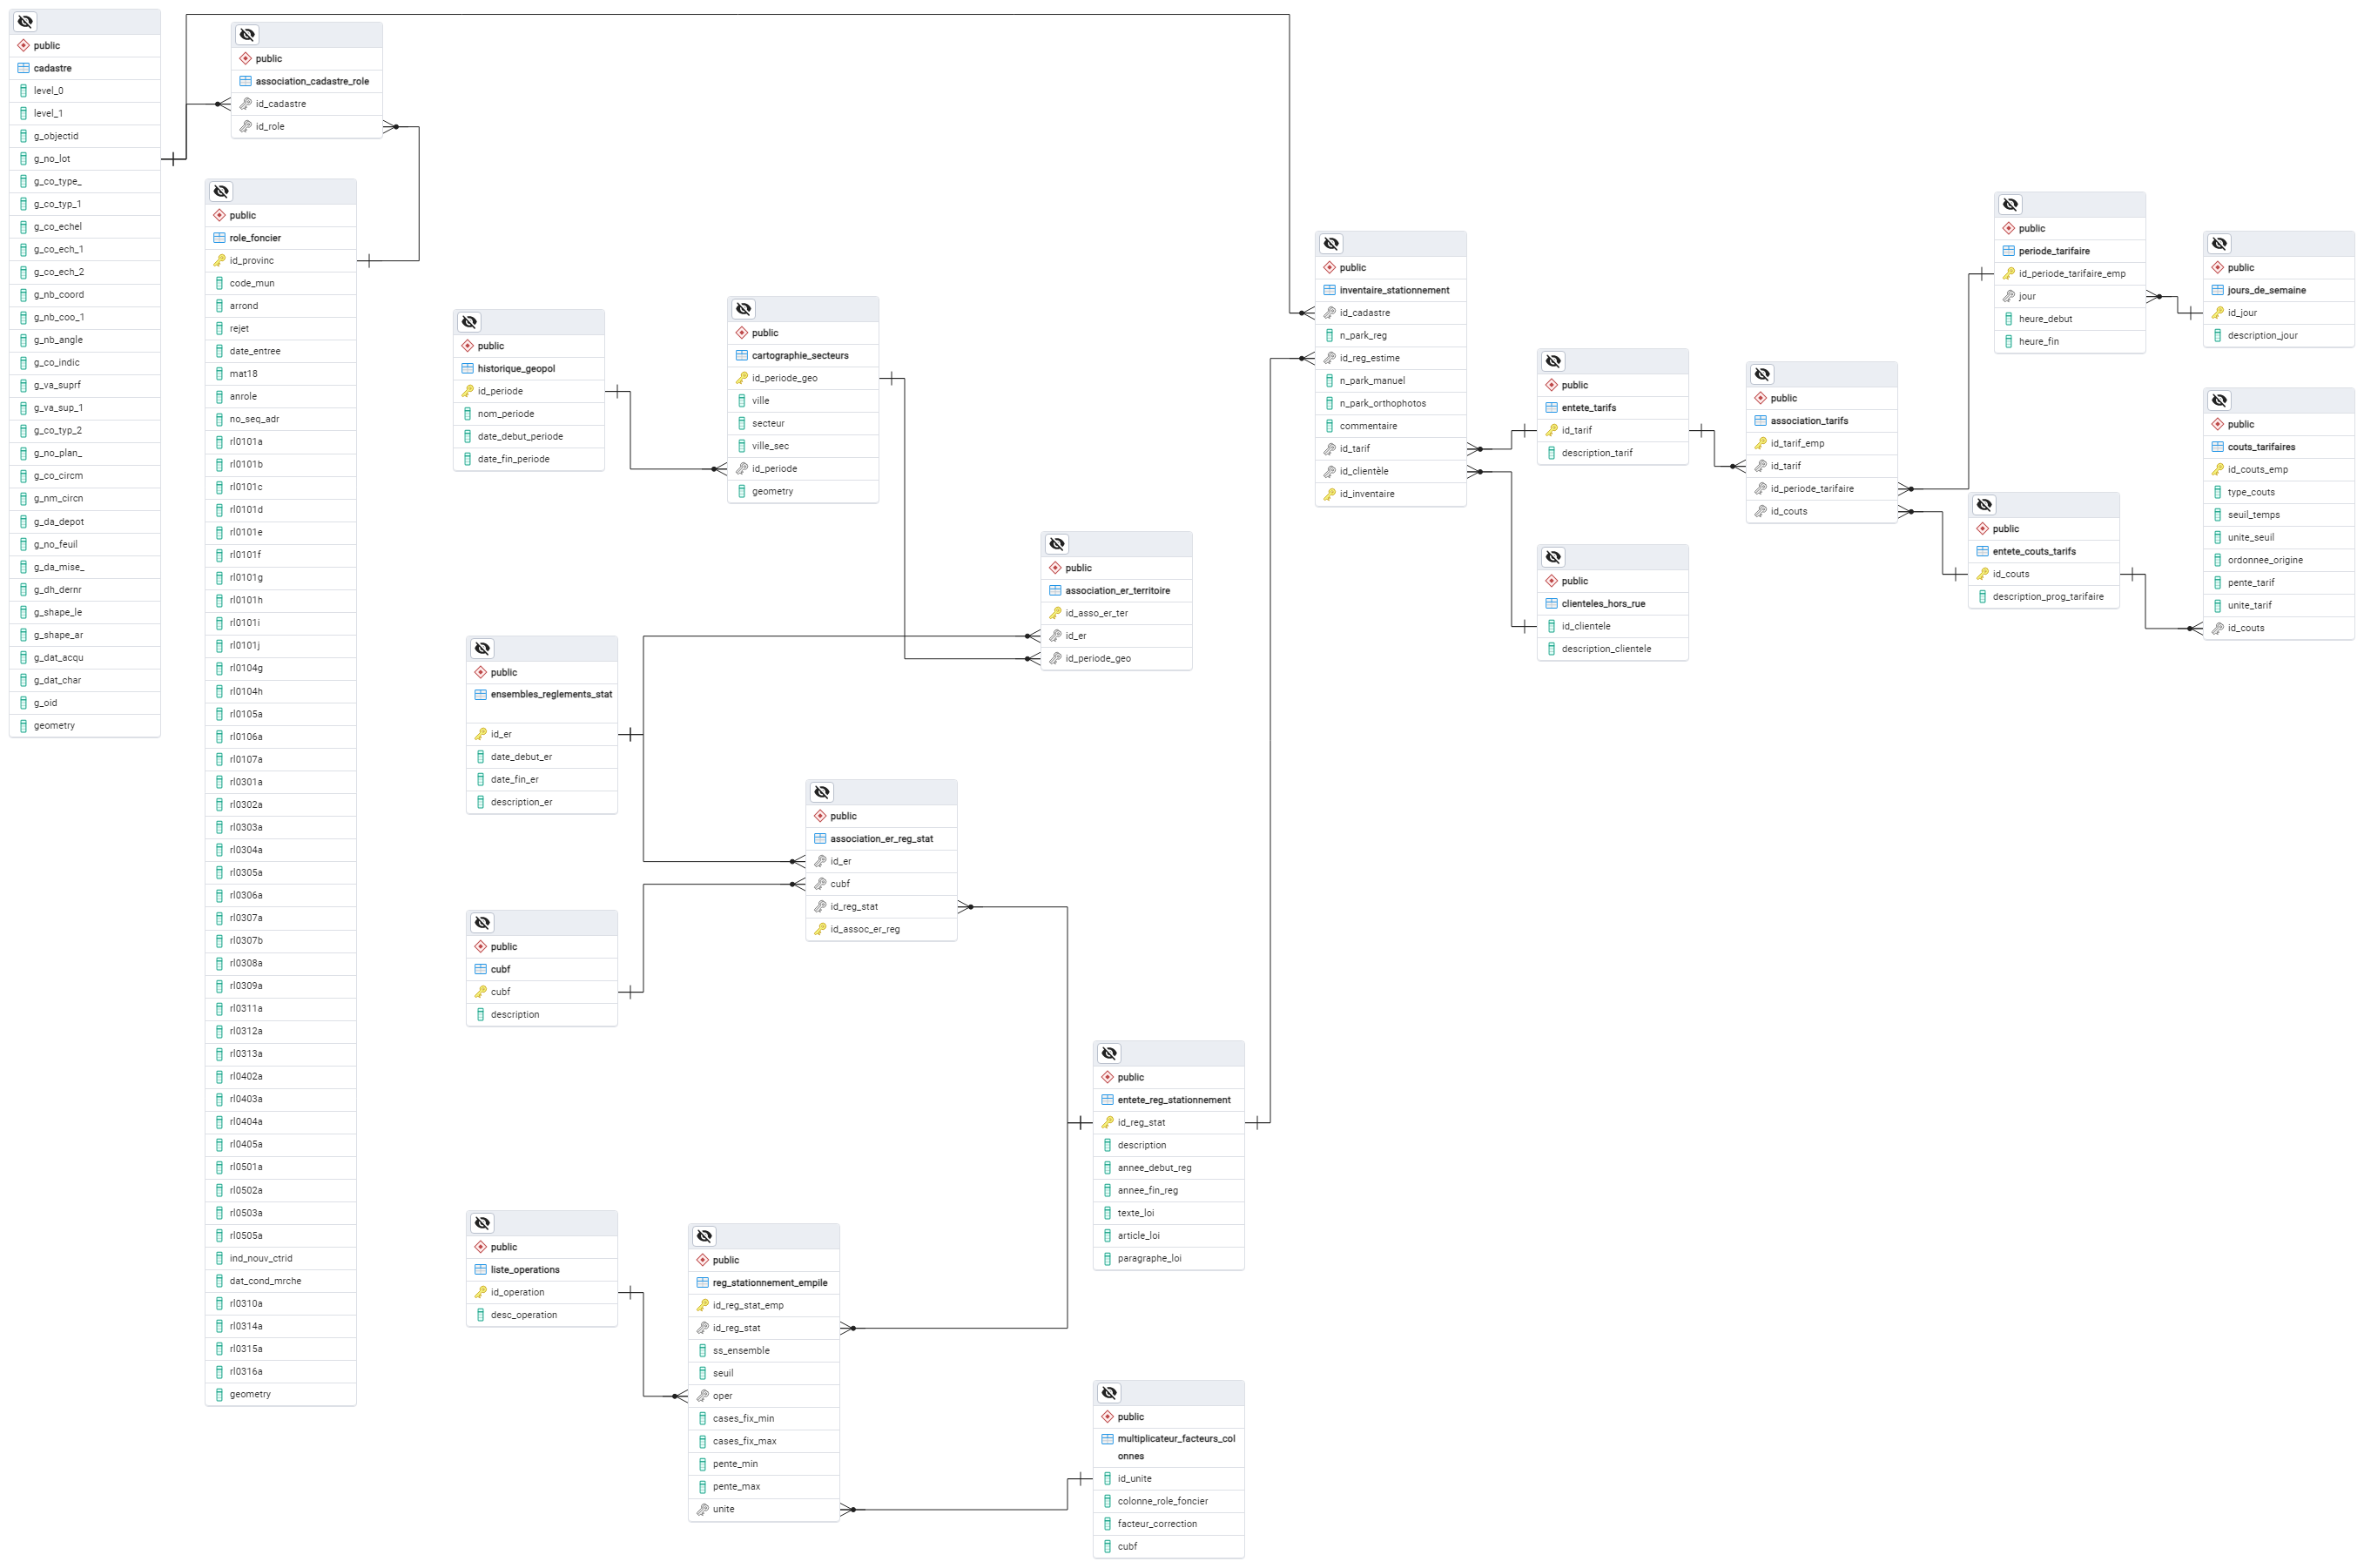
\includegraphics[trim={16cm 22cm 55cm 24cm},clip,width=12.5cm]{images/structure_base_de_donnee.png}
        \caption{Schéma relationnel pour la définition d'ensembles de règlements}
        \label{fig:offstreet_db_erd_rulesets}
    \end{figure}
    \FloatBarrier

    
    \subsubsection{Association du territoire aux ensembles de règlements}
    La table \underline{association\_er\_territoire} est nécessaire pour associer les territoires aux ensembles de règlements. Elle comporte trois champs: id\_asso\_er\_ter qui est la cle primaire, id\_er qui fait référence à la clé primaire de \underline{ensembles\_reglements\_stat} et id\_periode\_geo qui fait référence à la clé primaire de \underline{cartographie\_secteurs}. La figure \ref{fig:offstreet_db_erd_er_ter} montre les champs de la table.
    \begin{figure}[h]
        \centering
        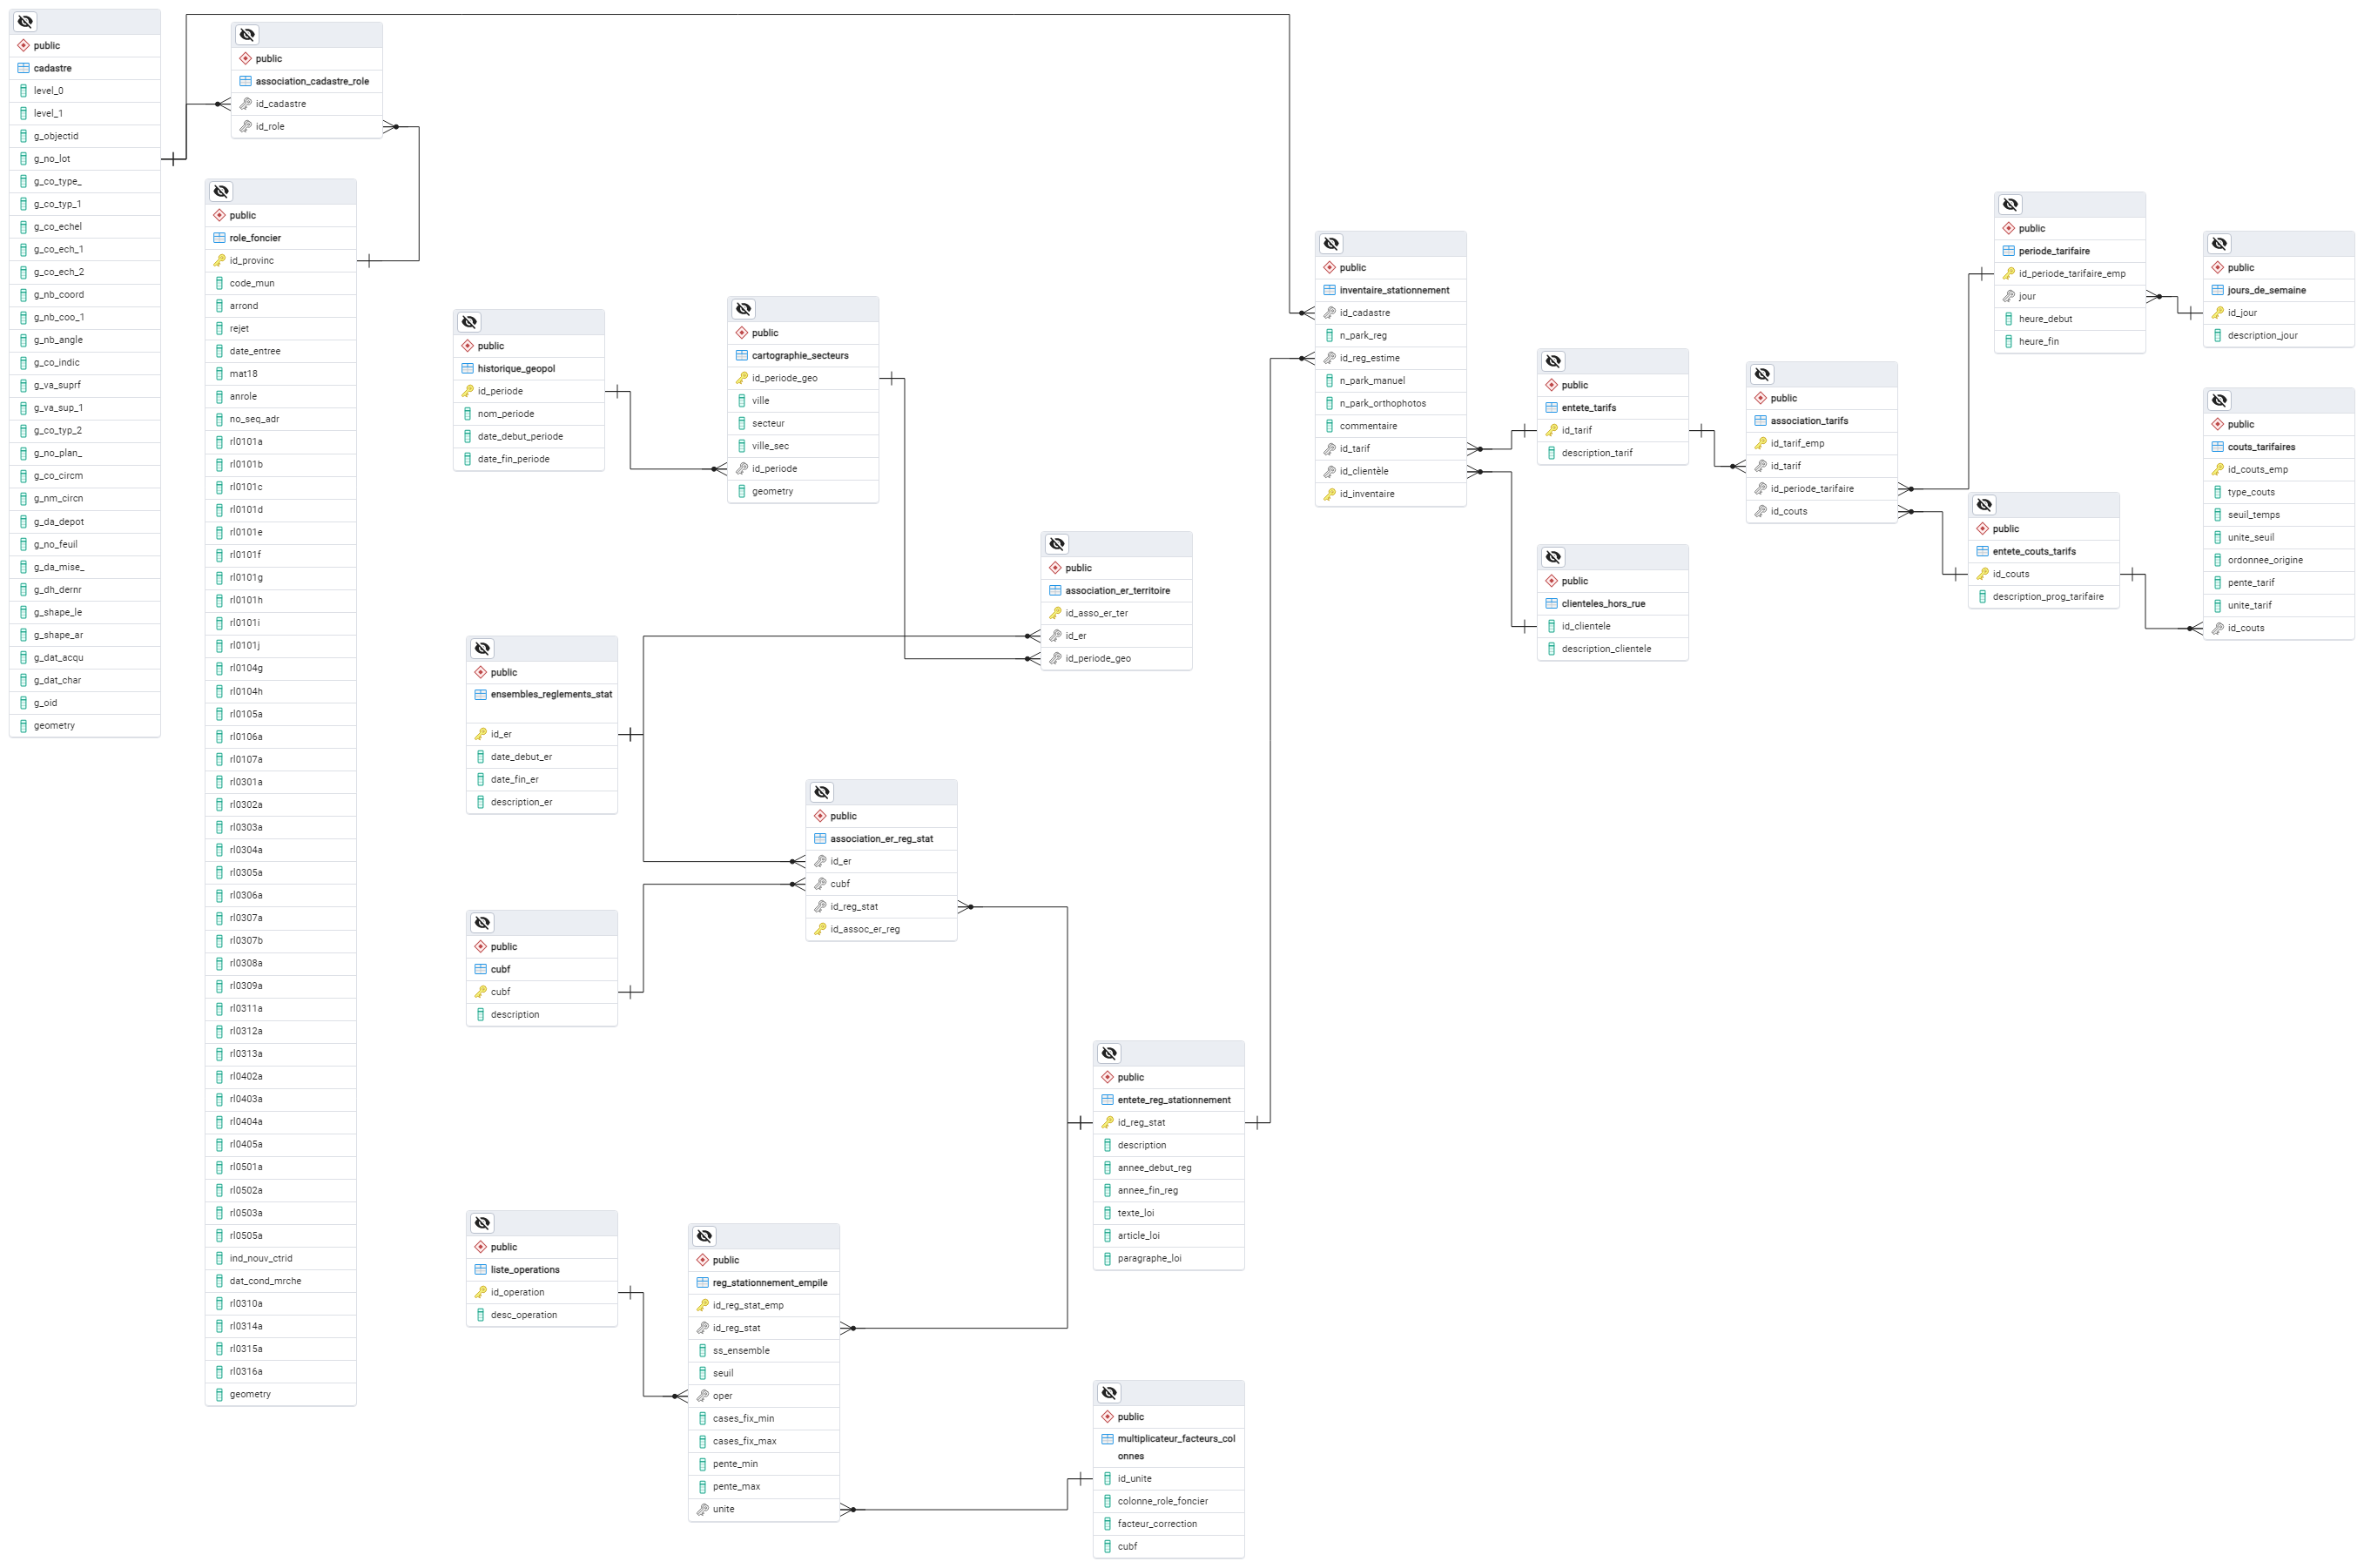
\includegraphics[trim={28cm 25cm 55cm 30cm},clip,width=5cm]{images/structure_base_de_donnee.png}
        \caption{Schéma relationnel pour l'association des règlements aux territoires}
        \label{fig:offstreet_db_erd_er_ter}
    \end{figure}
    \FloatBarrier

    
    \subsubsection{Données de départ}Les données de départ sont le rôle foncier brut ainsi que le cadastre représentés dans les tables \underline{cadastre} et \underline{role\_foncier}. Inclus dans ces tables sont l'ensemble des champs qui proviennent des données disponibles sur Géo-Index et Données Québec. \par
    Le cadastre est utilisé pour pouvoir améliorer la cartographie et la représentation des données sur une carte choroplèthe. La table \underline{association\_cadastre\_role} associe le cadastre avec le rôle foncier. En théorie, une jointure géométrique pourrait être complétée, mais celle-ci peut être onéreuse et mener à des erreurs pour des lots avec des formes concaves. L'approche faisant l'association dans une table permet de gérer ces formes sans manipulation une fois une première correction complétée. Ceci est différent de l'approche utilisée par la chaire, où les points du cadastre sur l'entrée principale du bâtiment. L'approche proposée ici permet d'utiliser les données brutes du cadastre qui sont issues de \textcite{GouvernementduQuebec:ManuelEvaluation:2024}. Clé primaire pour le cadastre est g\_no\_lot et la clé primaire pour le rôle est l'id\_provinc.\par
    La figure \ref{fig:offstreet_db_erd_input_data} montre les tables pertinentes en intrant. Il est concevable que ces tables soient entreposés dans un serveur différent si cette méthodologie était implémenté dans un milieu municipal.
    \begin{figure}[ht!]
        \centering
        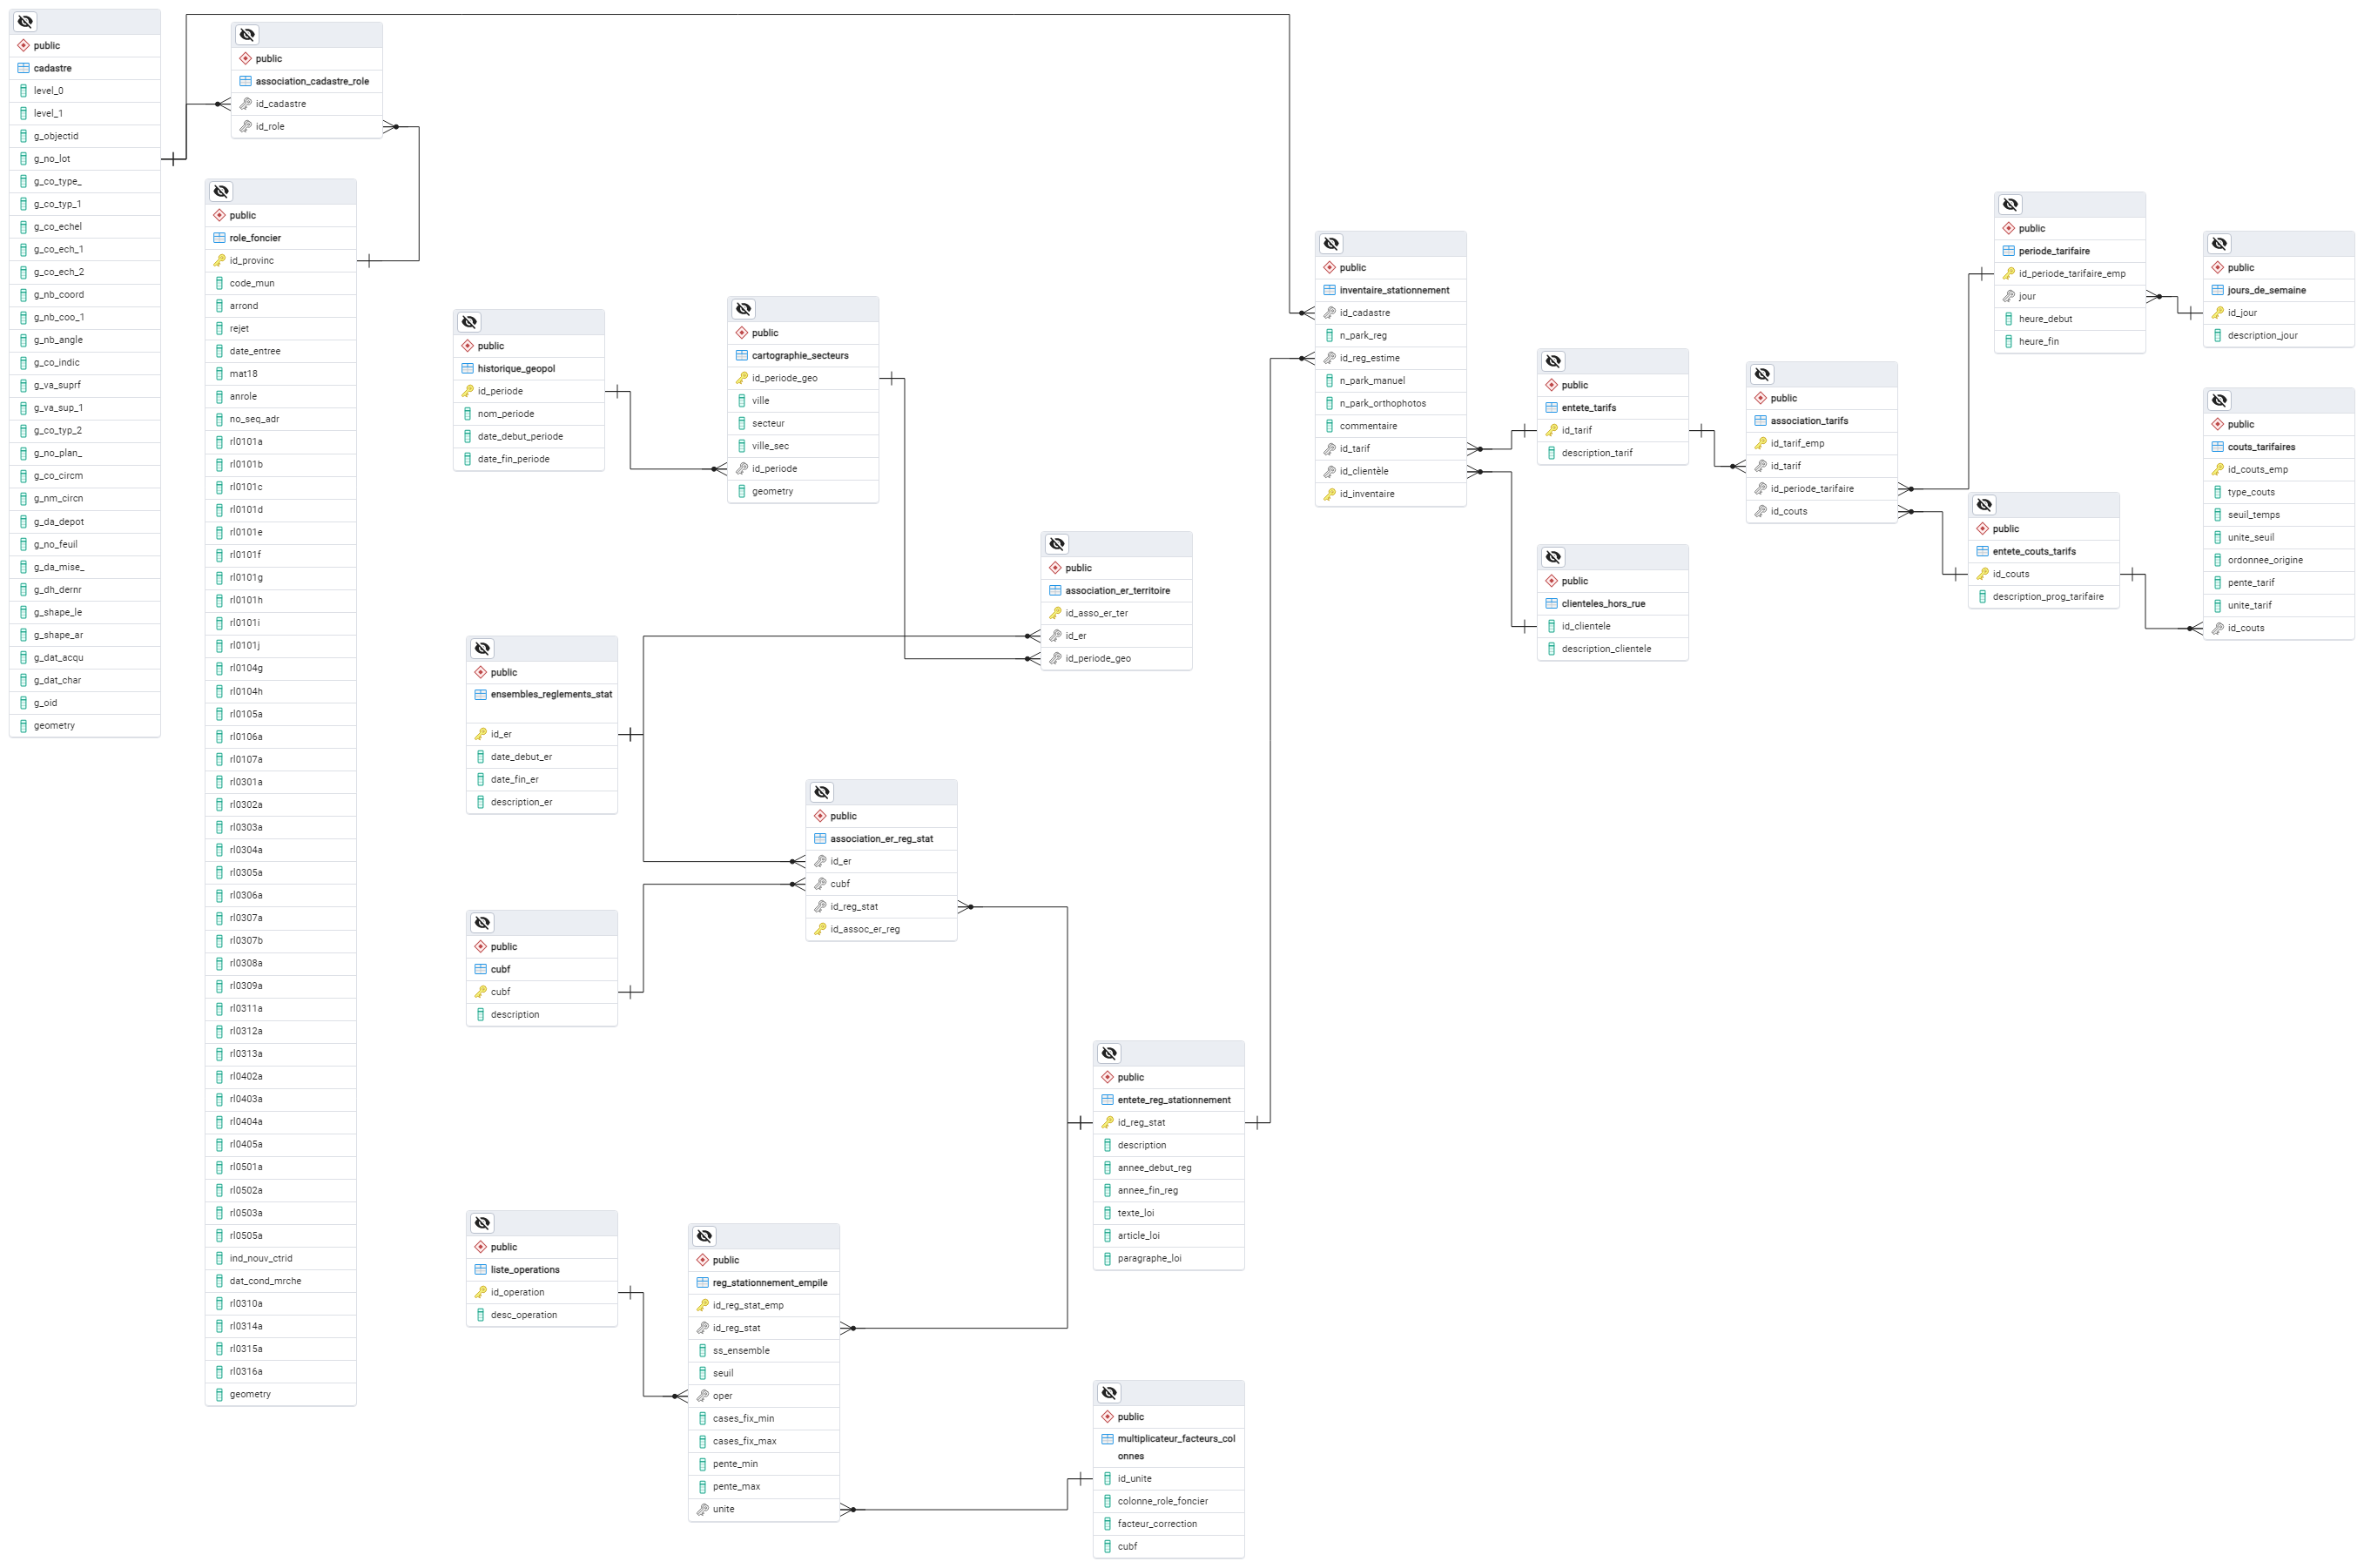
\includegraphics[trim={0cm 6cm 77.5cm 0cm},clip,height=20cm]{images/structure_base_de_donnee.png}
        \caption{Schéma relationnel pour le rôle foncier et le cadastre}
        \label{fig:offstreet_db_erd_input_data}
    \end{figure}
    \FloatBarrier
    
    \subsection{Calcul du nombre de places par méthode réglementaire}
        \subsubsection{Logigramme de la méthode globale}
        \subsubsection{Vérification de la base de données de stationnement}
            \paragraph{Validation des périodes de validité}
            \paragraph{Validation de couverture de l'ensemble des \ac{CUBF}}
        \subsubsection{Expansion des ensembles de règlements}
        \subsubsection{Sélection des propriétés à assigner: territoire et règlementation}
        \subsubsection{Gestion des propriétés non-assignées}
        \subsubsection{Inférence de la capacité de stationnement}
     
\section{Méthode d'inventaire hors rue basée sur les ortho-photographies}\label{sec:meth_orthophoto}
\section{Interface de programmation applicative}\label{sec:meth_API}
\section{Interface Web proposé} \label{sec:meth_interface_web}
\section{Méthode d'analyse} \label{sec:meth_analyse}
  \subsection{Analyse spatio temporelle de l'offre de stationnement}
  \subsection{Analyse spatio temporelle de la demande de stationnement}
  \subsection{Analyse d'utilisation de la ressource}
             %  "Détails de la Solution" (Maîtrise)
\Chapter{RÉSULTATS}\label{sec:Resultats}
Texte / Text.
          %  "Résultats théoriques et expérimentaux" (Maîtrise)
\Chapter{CONCLUSION}\label{sec:Conclusion}
Texte / Text.

%%
%%  SYNTHESE DES TRAVAUX / SUMMARY OF WORKS
%%
\section{Synthèse des travaux}
Texte / Text.

%%
%%  LIMITATIONS
%%
\section{Limitations de la solution proposée}\label{sec:Limitations}

%%
%%  AMELIORATIONS FUTURES / FUTURE RESEARCH
%%
\section{Améliorations futures}
Texte / Text.
         % Conclusion.
%\backmatter
%\ifthenelse{\equal{\Langue}{english}}{
%	\renewcommand\bibname{REFERENCES}
%	\bibliography{Document}
%	\bibliographystyle{IEEEtran}			% Style bibliographique / Bibliography style 
%}{
	\renewcommand\bibname{RÉFÉRENCES}
	\printbibliography{}
%	\bibliographystyle{apa-uqac-fr}    % Style bibliographique / Bibliography style 
%}
%
\ifthenelse{\equal{\AnnexesPresentes}{O}}{
	\appendix%
	\newcommand{\Annexe}[1]{\annexe{#1}\setcounter{figure}{0}\setcounter{table}{0}\setcounter{footnote}{0}}%
	%%
%%  Annexes
%%
%%  Note: Ne pas modifier la ligne ci-dessous. / Do not modify the following line.
\ifthenelse{\equal{\Langue}{english}}{
	\addcontentsline{toc}{compteur}{APPENDICES}
}{
	\addcontentsline{toc}{compteur}{ANNEXES}
}
%%
%%
%%  Toutes les annexes doivent être inclues dans ce document
%%  les unes à la suite des autres.
%%  All annexes must be included in this document one after the other.
\Annexe{Démo}
Texte de l'annexe A\@. Remarquez que la phrase précédente se termine
par une lettre majuscule suivie d'un point. On indique explicitement
cette situation à \LaTeX{} afin que ce dernier ajuste correctement
l'espacement entre le point final de la phrase et le début de la
phrase suivante.


\begin{landscape}
\Annexe{Encore une annexe / Another Appendix}
Texte de l'annexe B\@ en mode «landscape».
\end{landscape}

\Annexe{Une dernière annexe / The Last Appendix}
Texte de l'annexe C\@.
}
{}
\end{document}
